%=============================================================================
% Thesis Template in LaTex
%
% Time-stamp: <Mon 2016-04-04 08:52 juergen>
% File:  main.tex -- Main file of the template
% Author(s): Juergen Hackl <hackl@ibi.baug.ethz.ch>
%            Clemens Kielhauser <kielhauser@ibi.baug.ethz.ch>
%
% Creation:  27 Jan 2014
%
% Copyright (c) 2014 Infrastructure Management Group (IMG)
%               http://ibi.ethz.ch
%
% More information on LaTeX: http://www.latex-project.org/
%=============================================================================

% **************
% Basic settings
% **************

\newcommand{\mylaterality}{twoside}
% "oneside" or "twoside"
% Either you are creating a document which is printed on both, left pages
% and right pages (twoside) or you create a document which is printed
% on right pages only (oneside).

\newcommand{\mylanguage}{english,ngerman}
% "english,ngerman", "ngerman,english", ...
% NOTE: The *last* language is the active one!
% See babel documentation for further details.

\newcommand{\mycolorlinks}{false}  %% "true" or "false"
% Enables or disables colored links (hyperref package).

\newcommand{\mylinenumbering}{false}  %% "true" or "false"
% Enables or disables linenumbers (lineno package).

\newcommand{\myspacing}{false}  %% "true" or "false"
% Enables or disables doublespacing (setspace package).

% General metadata for the PDF
\newcommand{\myauthor}{Cyrano Golliez}  %% also used for PDF metadata (hyperref)
\newcommand{\myethnr}{15-914-609}
\newcommand{\mytitle}{Bedarfsgerechte Optimierung \\ der Veloinfrastruktur Uster}  %% also used for PDF metadata (hyperref)
\newcommand{\mysubject}{SUBJECT was kommt hier}  %% also used for PDF metadatay (hyperref)
\newcommand{\mykeywords}{KEYWORDS}  %% also used for PDF metadata (hyperref)
\newcommand{\myprofessor}{Prof. Dr. Bryan T. Adey}
\newcommand{\mysupervisor}{Dr. Claudio Martani}

% ********
% Preamble
% ********

% Load main settings for document preamble
% ========================================
%=============================================================================
% Thesis Template in LaTex
%
% Time-stamp: <Mon 2016-04-04 07:49 juergen>
% File:  main.tex -- Main file of the template
% Author(s): Juergen Hackl <hackl@ibi.baug.ethz.ch>
%            Clemens Kielhauser <kielhauser@ibi.baug.ethz.ch>
%
% Creation:  27 Jan 2014
%
% Copyright (c) 2014 Infrastructure Management Group (IMG)
%               http://ibi.ethz.ch
%
% More information on LaTeX: http://www.latex-project.org/
%=============================================================================

% ********
% Preamble
% ********

% Documentclass using KOMA-script
% ===============================

\documentclass[
  paper=a4,                         % Paper format
  fontsize=11pt,                    % Fontsize
  DIV=12,                           % Divided page horizontally and vertically
  BCOR=10mm,                        % Binding correction
  \mylaterality,                    % Double or one-sided typesetting
  parskip=half,                     % Parskip
]{scrreprt}                         % KOMA - class


% Usepackages
% ===========

\usepackage[utf8]{inputenc}         % Input caracters
\usepackage[T1]{fontenc}            % Font encodings
\usepackage[ngerman]{babel}         % Language
\usepackage{scrpage2}               % Headers and footers
\pagestyle{scrheadings}             % Headers and footers
\usepackage{graphicx}               % Enhanced support for graphics
\usepackage[export]{adjustbox}
\usepackage{xcolor}                 % Color extensions
\usepackage{enumitem}               % Layout of itemize, enumerate, ...
\usepackage{multicol}               % Multiple columns
\usepackage{subfig}                 % Figures broken into subfigures
\usepackage{rotating}               % Rotation tools
\usepackage{longtable}              % Long tables
\usepackage{tabularx}               % Adjustable Tabulars
\usepackage{booktabs}               % Tabular rules
\usepackage{float}                  % Float environment
\usepackage{amsmath}                % AMS mathematical facilities
\usepackage{amssymb}                % AMS symbol fonts
\usepackage{makeidx}                % Index
\usepackage[intoc]{nomencl}         % Nomenclature
\usepackage{acronym}                % Acronyms
\usepackage{tikz}                   % TikZ
\usepackage{pgfplots}               % PGF plots
\usepackage{units}                  % Typeset units
\usepackage{csquotes}               % quotes
\usepackage{wasysym}                % Additional Symbols
\usepackage{listings}
\usepackage{pgfgantt}               % Gantt Chart
\usepackage{pdfpages}               % Includes PDF files
\usepackage{blindtext}              % Some random text
\usepackage{ifthen}                 % If commands

% BibLaTeX using biber as backend (recommended)
% ---------------------------------------------

% \usepackage[authordate,backend=biber]{biblatex-chicago}
% \bibliography{literature}
% \setlength\bibitemsep{1.5\itemsep}


% BibTeX
% ------

% \usepackage{cite}                   % Citations
\usepackage{natbib}                 % Citation Style
% \usepackage{apacite}                % APA cite Style
% \renewcommand{\bibsection}{}        % No auto headings


% Line spacing
% ------------
\ifthenelse{\equal{\myspacing}{true}}
{
\usepackage[doublespacing]{setspace} % Set line space to 2
}{}
% \usepackage[onehalfspacing]{setspace} % Set line space to 1.5


% Line numbering
% --------------

\usepackage{lineno}    % numbering the lines
\ifthenelse{\equal{\mylinenumbering}{true}}{\linenumbers}{}


% Font settings
% -------------

% \usepackage[scaled]{helvet}
% \renewcommand*\familydefault{\sfdefault}


% PDF settings
% ------------

\usepackage[
  pdftitle={\mytitle},
  pdfauthor={\myauthor},
  pdfsubject={\mysubject},
  pdfcreator={Accomplished with: pdfLaTeX, biber, tikz and hyperref-package},
  pdfproducer={\myauthor},
  pdfkeywords={\mykeywords},
  a4paper=true,
  pdftex=true,
  backref,
  pagebackref=false,                % creates backward references too
  bookmarks=false,                  %
  bookmarksopen=false,              % Bookmarkcolumn is opened
  pdfpagemode=None,                 % None, UseOutlines, UseThumbs, FullScreen
  plainpages=false,                 %
  pdfdisplaydoctitle=true,          % show documenttitle
  colorlinks=\mycolorlinks,                  % turn on/off colored links
]{hyperref}

% Header
% ======

\automark[section]{chapter}


% Table rule
% ----------

\renewcommand{\arraystretch}{2}
\setlength{\arrayrulewidth}{1pt}
\lightrulewidth=1pt
\heavyrulewidth=.5pt


% Colors
% ======

\definecolor{ibiBlue}{RGB}{0,106,175}
\definecolor{ethBlue}{RGB}{31,64,122}
\definecolor{ethLightBlue}{RGB}{18,105,176}
\definecolor{ethGreen}{RGB}{72,90,44}
\definecolor{ethLightGreen}{RGB}{154,197,15}
\definecolor{ethGray}{RGB}{111,111,100}
\definecolor{ethRed}{RGB}{168,50,45}
\definecolor{ethLogo}{RGB}{0,0,0}%{255, 255, 255}
\definecolor{DBaugGreen}{RGB}{169,200,61}
\definecolor{DBaugBlue}{RGB}{42,105,182}

% Hyphenations
% =============

\hyphenation{ex-am-ple hy-phen-ate}


% MISC
% ====
\raggedbottom
\makeindex

\newenvironment{IMleftskip}{\par\begingroup\leftskip=2em}{\par\endgroup}
\newenvironment{IMleftrightskip}{\par\begingroup\leftskip=2em\rightskip=2em}{\par\endgroup}

%=============================================================================
%%% Local Variables:
%%% mode: latex
%%% TeX-master: "main"
%%% End: %% DO NOT REMOVE THIS LINE!

%=============================================================================

% *************
% Main Document
% *************

% Document
% ========

\begin{document}

% roman page numbers
% ------------------
%\frontmatter
\pagenumbering{roman}

% Titlepage
% ---------
%=============================================================================
% Thesis Template in LaTex
%
% Time-stamp: <Mon 2016-04-04 08:51 juergen>
% File:  00-01-b-Titlepage.tex -- Titlepage for a thesis
% Author(s): Juergen Hackl <hackl@ibi.baug.ethz.ch>
%            Clemens Kielhauser <kielhauser@ibi.baug.ethz.ch>
%
% Creation:  27 Jan 2014
%
% Copyright (c) 2014 Infrastructure Management Group (IMG)
%               http://www.ibi.ethz.ch
%
% More information on LaTeX: http://www.latex-project.org/
%=============================================================================


\begin{titlepage}

%=============================================================================
% Thesis Template in LaTex
%
% File:  f-00-00-Background.tex -- Background of the titlepage
% Author(s): Juergen Hackl <hackl@ibi.baug.ethz.ch>
%            Clemens Kielhauser <kielhauser@ibi.baug.ethz.ch>
%
% Creation:  27 Jan 2014
% Time-stamp: <Tue 2013-08-13 20:14 juergen>
%
% Copyright (c) 2014 Infrastructure Management Group (IMG)
%               http://www.ibi.ethz.ch
%
% More information on LaTeX: http://www.latex-project.org/
%=============================================================================

\begin{tikzpicture}[remember picture,overlay,]

\node [xshift=0mm,yshift=0mm] at (current page.north west)(p1) {};
\node [xshift=0mm,yshift=0mm] at (current page.south east)(p2) {};
\fill [fill=white] (p1)rectangle(p2);

\node [xshift=7mm,yshift=-7mm] at (current page.north west)(t1) {};
\node [xshift=-7mm,yshift=-38mm] at (current page.north east)(t2) {};
\fill [fill=ethLightGreen] (t1)rectangle(t2);


\begin{scope}[yshift=13.5mm,xshift=-10.5mm,y=0.80pt, x=0.8pt,yscale=-1, inner sep=0pt, outer sep=0pt]
\begin{scope}[cm={{1.25,0.0,0.0,-1.25,(0.0,28.575)}}]
  \begin{scope}[scale=0.100]
    \path[fill=ethLogo,nonzero rule] (864.9840,62.3398) .. controls
      (856.8870,22.1719) and (825.8550,20.1289) .. (819.7070,20.1289) .. controls
      (802.1880,20.1289) and (791.7380,30.2500) .. (791.7380,47.1719) .. controls
      (791.7380,51.0352) and (792.3050,56.2930) .. (793.2850,61.5625) --
      (812.4800,157.1760) -- (812.5630,157.5430) -- (789.8950,157.5430) --
      (770.3360,59.4961) -- (770.0780,58.0938) .. controls (769.2380,53.6680) and
      (768.4530,49.4688) .. (768.4530,44.0195) .. controls (768.4530,17.6758) and
      (785.7540,0.0000) .. (811.5390,0.0000) .. controls (830.3980,0.0000) and
      (845.5470,6.1875) .. (856.6090,18.4063) -- (853.6720,2.2578) --
      (853.5980,1.8750) -- (875.9450,1.8750) -- (906.8320,157.1760) --
      (906.8950,157.5430) -- (883.9020,157.5430) -- (864.9840,62.3398);
    \path[fill=ethLogo,nonzero rule] (1019.5400,159.4340) .. controls
      (1002.0200,159.4340) and (986.4920,152.2700) .. (976.7230,139.6950) --
      (980.2340,157.1760) -- (980.3050,157.5430) -- (957.9490,157.5430) --
      (927.0630,2.2578) -- (926.9880,1.8750) -- (949.6800,1.8750) --
      (968.5900,97.1172) .. controls (973.4220,121.5660) and (992.1910,139.2970) ..
      (1013.2400,139.2970) .. controls (1022.2800,139.2970) and (1029.4000,135.7300)
      .. (1035.0000,128.4220) -- (1035.2100,128.1410) -- (1053.6200,144.6290) --
      (1053.4300,144.8630) .. controls (1044.9300,154.6880) and (1033.8300,159.4340)
      .. (1019.5400,159.4340);
    \path[fill=ethLogo,nonzero rule] (644.6840,137.7970) -- (644.6130,137.4100) --
      (721.9730,137.4100) -- (618.9800,20.9688) -- (618.9260,20.9063) --
      (615.0430,1.8750) -- (724.8240,1.8750) -- (728.7300,22.0156) --
      (646.6640,22.0156) -- (749.9770,138.4650) -- (750.0230,138.5350) --
      (753.8950,157.5430) -- (648.5230,157.5430) -- (644.6840,137.7970);
    \path[fill=ethLogo,nonzero rule] (1056.5000,2.2578) -- (1056.4300,1.8750) --
      (1079.1000,1.8750) -- (1110.0300,157.5430) -- (1087.7300,157.5430) --
      (1056.5000,2.2578);
    \path[fill=ethLogo,nonzero rule] (1363.9100,159.4220) .. controls
      (1345.2600,159.4220) and (1330.7000,153.7110) .. (1319.5100,141.9300) --
      (1337.0900,228.6130) -- (1314.4100,228.6130) -- (1268.8600,1.8555) --
      (1291.5400,1.8555) -- (1310.4400,97.1094) .. controls (1318.5500,137.2620) and
      (1349.8600,139.2930) .. (1356.0400,139.2930) .. controls (1373.3700,139.2930)
      and (1383.7300,129.1800) .. (1383.7300,112.2500) .. controls
      (1383.7300,108.4140) and (1383.1400,103.1760) .. (1382.1400,97.8516) --
      (1362.9100,1.8555) -- (1385.5600,1.8555) -- (1405.4400,99.9414) .. controls
      (1406.4000,105.1560) and (1407.0400,109.5590) .. (1407.0400,115.4100) ..
      controls (1407.0400,141.7380) and (1389.6800,159.4220) ..
      (1363.9100,159.4220);
    \path[fill=ethLogo,nonzero rule] (1213.6000,159.4340) .. controls
      (1172.4700,159.4340) and (1143.6000,130.4570) .. (1134.3700,79.9414) ..
      controls (1132.7100,71.4805) and (1132.1300,62.0156) .. (1132.1300,55.9727) ..
      controls (1132.1300,21.4492) and (1153.0900,0.0000) .. (1186.8500,0.0000) ..
      controls (1206.4800,0.0000) and (1224.4000,7.5234) .. (1238.6600,21.7734) --
      (1238.8600,21.9883) -- (1225.7900,37.9375) -- (1225.5500,38.2227) --
      (1225.3100,37.9531) .. controls (1213.2800,25.2969) and (1202.5000,20.1289) ..
      (1188.1000,20.1289) .. controls (1172.0100,20.1289) and (1154.8000,29.7070) ..
      (1154.8000,56.6055) .. controls (1154.8000,65.0234) and (1155.8000,71.9805) ..
      (1157.2900,79.8242) .. controls (1159.7200,93.0234) and (1165.1900,111.4650)
      .. (1177.3400,124.2930) .. controls (1187.0000,134.2460) and
      (1198.4500,139.2970) .. (1211.4000,139.2970) .. controls (1224.9200,139.2970)
      and (1233.3700,134.4880) .. (1241.6200,122.1480) -- (1241.8100,121.8400) --
      (1258.4500,135.9020) -- (1258.6900,136.0980) -- (1258.5100,136.3520) ..
      controls (1247.1400,152.3240) and (1233.2900,159.4340) ..
      (1213.6000,159.4340);
    \path[fill=ethLogo,nonzero rule] (1096.1500,200.2700) -- (1118.8700,200.2700) --
      (1124.5200,228.6130) -- (1101.8800,228.6130) -- (1096.1500,200.2700);
    \path[fill=ethLogo,nonzero rule] (875.6800,200.2700) -- (898.4060,200.2700) --
      (904.0310,228.6130) -- (881.4220,228.6130) -- (875.6800,200.2700);
    \path[fill=ethLogo,nonzero rule] (815.2150,200.2700) -- (837.9380,200.2700) --
      (843.5740,228.6130) -- (820.9610,228.6130) -- (815.2150,200.2700);
    \path[fill=ethLogo,nonzero rule] (512.2890,140.7460) -- (461.2730,140.7460) --
      (479.1880,228.6130) -- (45.5430,228.6130) -- (0.0000,1.8555) --
      (172.8980,1.8555) -- (184.2230,58.5352) -- (82.1406,58.5352) --
      (88.3320,89.7188) -- (190.3830,89.7188) -- (200.6520,140.7460) --
      (98.5781,140.7460) -- (104.7620,171.9340) -- (266.5630,171.9340) --
      (232.4020,1.8555) -- (303.2700,1.8555) -- (337.4260,171.9340) --
      (396.9260,171.9340) -- (362.7700,1.8555) -- (433.6480,1.8555) --
      (451.1370,89.7188) -- (502.1450,89.7188) -- (484.6520,1.8555) --
      (555.5200,1.8555) -- (601.0780,228.6130) -- (530.2110,228.6130) --
      (512.2890,140.7460);
  \end{scope}
\end{scope}
\end{scope}

\node [xshift=16mm,yshift=-31mm] at (current page.north west)(n1) {};
\node [xshift=-16mm,yshift=-89.75mm] at (current page.north east)(n2) {};
\fill [fill=ethLightBlue] (n1)rectangle(n2);

\node [xshift=16mm,yshift=-89.75mm] at (current page.north west)(n3) {};
\node [xshift=-16mm,yshift=-266mm] at (current page.north east)(n4) {};
\fill [fill=white] (n3)rectangle(n4);

        \begin{scope}[xshift=-9.5mm,yshift=-249mm,yscale=-.09,xscale=.09]
%          \fill[ibiBlue] (0,0) rectangle ++ (4,4);
          \fill[ibiBlue] (0,5) rectangle ++ (4,4);
          \fill[ibiBlue] (0,10) rectangle ++ (4,4);
          \fill[ibiBlue] (5,0) rectangle ++ (4,4);
          \fill[ibiBlue] (5,5) rectangle ++ (4,4);
          \fill[ibiBlue] (5,10) rectangle ++ (4,4);
          \fill[ibiBlue] (10,0) rectangle ++ (4,4);
          \fill[ibiBlue] (10,5) rectangle ++ (4,4);
          \fill[ibiBlue] (10,10) rectangle ++ (4,4);
          \begin{scope}[rotate=-20]
            \fill[ibiBlue] (0,0) rectangle ++ (4,-4);
          \end{scope}
        \begin{scope}[xshift=150mm,yshift=30mm]
          \node (a1) at (0,0) [anchor=west,font=\scriptsize] {\sf {\textbf{Institut für Bau- und}}};
          \node (a2) at (0,4) [anchor=west,font=\scriptsize] {\sf {\textbf{Infrastrukturmanagement}}};
          \node (a3) at (0,8) [anchor=west,font=\scriptsize] {\sf {{Professur für Infrastrukturmanagement}}};
%          \node (a4) at (0,12) [anchor=west,font=\scriptsize] {\sf {{}}};
%          \node (a5) at (0,16) [anchor=west,font=\scriptsize] {\sf {{}}};
        \end{scope}
        \end{scope}

\begin{scope}[xshift=60mm,yshift=-173mm]
\begin{scope}[y=1pt,x=1pt,yscale=-.15, xscale=.15, inner sep=0pt, outer sep=0pt]
  \begin{scope}
    \begin{scope}[cm={{0.51378,0.0,0.0,0.51378,(272.38882,1217.1677)}}]
      \path[fill=DBaugGreen] (668.5714,876.7307) .. controls (668.5714,872.5367) and
        (687.9638,846.0362) .. (701.7970,831.3265) -- (708.1448,824.5765) --
        (720.7991,824.5765) .. controls (727.7589,824.5765) and (733.6630,824.9157) ..
        (733.9193,825.3304) .. controls (734.1756,825.7450) and (731.2415,829.9075) ..
        (727.3992,834.5804) .. controls (718.7720,845.0722) and (709.2663,858.5392) ..
        (703.0449,869.0837) .. controls (700.4512,873.4797) and (697.8211,877.4071) ..
        (697.2002,877.8112) .. controls (696.5794,878.2153) and (689.8839,878.5528) ..
        (682.3214,878.5612) .. controls (669.6154,878.5753) and (668.5714,878.4363) ..
        (668.5714,876.7307) -- cycle(705.8214,877.9142) .. controls
        (705.1339,877.6368) and (704.5714,876.9473) .. (704.5714,876.3820) .. controls
        (704.5714,873.0693) and (724.6375,843.1986) .. (734.7765,831.4183) --
        (740.6650,824.5765) -- (759.6182,824.5765) .. controls (770.7387,824.5765) and
        (778.5714,824.9638) .. (778.5714,825.5136) .. controls (778.5714,826.0290) and
        (776.0579,830.4165) .. (772.9858,835.2636) .. controls (769.9137,840.1107) and
        (763.7262,851.5758) .. (759.2358,860.7417) .. controls (753.5524,872.3428) and
        (750.4636,877.5805) .. (749.0714,877.9780) .. controls (746.6255,878.6765) and
        (707.5677,878.6189) .. (705.8214,877.9142) -- cycle(760.6119,877.7106) ..
        controls (759.3576,876.8416) and (759.4854,875.8826) .. (761.5217,870.8880) ..
        controls (765.0374,862.2644) and (774.7665,843.0005) .. (780.5594,833.1930) --
        (785.6488,824.5765) -- (808.5511,824.5765) .. controls (821.1473,824.5765) and
        (831.6714,824.9293) .. (831.9380,825.3606) .. controls (832.2045,825.7918) and
        (830.9210,830.6293) .. (829.0857,836.1106) .. controls (827.2504,841.5918) and
        (823.9032,852.8097) .. (821.6475,861.0391) .. controls (819.3917,869.2686) and
        (817.1653,876.3825) .. (816.7000,876.8479) .. controls (815.4274,878.1205) and
        (762.3813,878.9364) .. (760.6119,877.7106) -- cycle(827.0274,876.3225) ..
        controls (826.4705,874.8711) and (834.2740,842.7434) .. (837.7743,832.0765) --
        (840.0714,825.0765) -- (865.2486,824.8095) .. controls (888.6045,824.5618) and
        (890.4599,824.6703) .. (890.8968,826.3095) .. controls (891.1559,827.2813) and
        (891.0761,839.1015) .. (890.7196,852.5765) -- (890.0714,877.0765) --
        (858.7955,877.3408) .. controls (834.0817,877.5496) and (827.4163,877.3358) ..
        (827.0274,876.3225) -- cycle(900.2409,876.8265) .. controls
        (899.9942,876.4140) and (899.6301,864.6015) .. (899.4319,850.5765) --
        (899.0714,825.0765) -- (924.2079,824.8096) .. controls (947.4512,824.5627) and
        (949.3974,824.6757) .. (950.0482,826.3096) .. controls (953.1514,834.1009) and
        (963.5714,872.4084) .. (963.5714,876.0256) .. controls (963.5714,877.3939) and
        (959.8696,877.5765) .. (932.1304,877.5765) .. controls (914.8379,877.5765) and
        (900.4876,877.2390) .. (900.2409,876.8265) -- cycle(1032.5471,863.5281) ..
        controls (1028.6765,855.8014) and (1022.3735,844.3567) .. (1018.5405,838.0953)
        .. controls (1014.7075,831.8338) and (1011.5714,826.2306) ..
        (1011.5714,825.6437) .. controls (1011.5714,824.9250) and (1017.7575,824.5765)
        .. (1030.5151,824.5765) -- (1049.4587,824.5765) -- (1057.8349,834.8265) ..
        controls (1070.6200,850.4717) and (1085.5714,872.7965) .. (1085.5714,876.2416)
        .. controls (1085.5714,877.3161) and (1081.0860,877.5765) ..
        (1062.5781,877.5765) -- (1039.5848,877.5765) -- cycle(1091.2381,875.3265) ..
        controls (1080.3637,857.5887) and (1070.7986,844.1510) .. (1061.4026,833.4116)
        .. controls (1058.1954,829.7459) and (1055.5714,826.2584) ..
        (1055.5714,825.6616) .. controls (1055.5714,824.9377) and (1059.8516,824.5765)
        .. (1068.4288,824.5765) -- (1081.2863,824.5765) -- (1089.7196,833.3265) ..
        controls (1094.3579,838.1390) and (1101.0255,845.6765) .. (1104.5365,850.0765)
        .. controls (1112.4695,860.0183) and (1122.6679,875.6114) ..
        (1121.9727,876.7362) .. controls (1121.6871,877.1984) and (1114.9653,877.5765)
        .. (1107.0354,877.5765) .. controls (1093.1589,877.5765) and
        (1092.5657,877.4920) .. (1091.2381,875.3265) -- cycle(720.5714,814.6408) ..
        controls (720.5714,813.3669) and (739.0070,800.0445) .. (750.1226,793.2857) ..
        controls (755.1007,790.2587) and (763.7874,785.4507) .. (769.4264,782.6012) --
        (779.6790,777.4203) -- (789.8752,777.4596) .. controls (795.4831,777.4812) and
        (805.3589,777.2526) .. (811.8214,776.9516) .. controls (824.9106,776.3420) and
        (826.3883,777.1452) .. (820.3214,781.5716) .. controls (813.3023,786.6928) and
        (803.4816,796.0480) .. (795.1141,805.5841) -- (786.3463,815.5765) --
        (768.9589,815.5765) .. controls (755.6373,815.5765) and (751.5714,815.2817) ..
        (751.5714,814.3158) .. controls (751.5714,813.0609) and (762.0937,803.6557) ..
        (772.5714,795.5453) .. controls (782.3377,787.9855) and (781.7808,787.7595) ..
        (771.0910,794.9444) .. controls (767.8017,797.1552) and (760.4982,802.7018) ..
        (754.8610,807.2702) -- (744.6114,815.5765) -- (732.5914,815.5765) .. controls
        (725.7956,815.5765) and (720.5714,815.1698) .. (720.5714,814.6408) --
        cycle(794.1011,814.6245) .. controls (792.9526,812.7662) and
        (810.0844,793.6477) .. (822.4740,782.9614) -- (829.8766,776.5765) --
        (842.6650,776.5765) .. controls (850.3282,776.5765) and (855.7075,776.9877) ..
        (856.0875,777.6025) .. controls (856.4363,778.1668) and (854.6262,781.8793) ..
        (852.0653,785.8525) .. controls (849.5043,789.8257) and (845.1255,797.8015) ..
        (842.3346,803.5765) .. controls (839.5437,809.3515) and (836.7677,814.4071) ..
        (836.1658,814.8111) .. controls (834.5186,815.9170) and (794.7909,815.7407) ..
        (794.1011,814.6245) -- cycle(844.9126,814.0232) .. controls
        (844.2258,812.2335) and (847.9295,802.9073) .. (854.3162,790.3444) .. controls
        (861.8293,775.5657) and (860.2747,776.4773) .. (877.4146,776.8003) --
        (892.0714,777.0765) -- (891.7001,795.0765) .. controls (891.4958,804.9814) and
        (890.8786,813.6386) .. (890.3277,814.3265) .. controls (889.5816,815.2580) and
        (883.7441,815.5765) .. (867.4176,815.5765) .. controls (848.5319,815.5765) and
        (845.4264,815.3621) .. (844.9126,814.0232) -- cycle(898.7400,813.8451) ..
        controls (898.2330,812.8724) and (897.6502,804.2015) .. (897.4448,794.5765) --
        (897.0714,777.0765) -- (911.7282,776.8003) -- (926.3850,776.5241) --
        (928.5898,779.3003) .. controls (931.5970,783.0867) and (944.4447,809.4739) ..
        (944.7917,812.5765) -- (945.0714,815.0765) -- (922.3666,815.3451) .. controls
        (901.5065,815.5919) and (899.5868,815.4701) .. (898.7400,813.8451) --
        cycle(1002.3978,814.3265) .. controls (1001.5421,813.6390) and
        (997.1550,808.9160) .. (992.6489,803.8310) .. controls (988.1427,798.7459) and
        (979.9819,790.8709) .. (974.5137,786.3310) .. controls (969.0456,781.7910) and
        (964.5716,777.7023) .. (964.5715,777.2449) .. controls (964.5715,776.7876) and
        (970.3089,776.6428) .. (977.3214,776.9232) .. controls (992.7489,777.5400) and
        (990.4952,777.5394) .. (999.7429,776.9302) -- (1007.4144,776.4244) --
        (1020.2429,782.9795) .. controls (1040.9110,793.5404) and (1069.4160,812.4013)
        .. (1068.0499,814.6118) .. controls (1067.7218,815.1426) and
        (1062.3731,815.5769) .. (1056.1638,815.5769) -- (1044.8743,815.5769) --
        (1035.4728,807.9410) .. controls (1030.3020,803.7412) and (1022.9214,798.1958)
        .. (1019.0714,795.6178) .. controls (1007.5819,787.9245) and
        (1006.6755,787.7578) .. (1016.0714,795.0661) .. controls (1027.7027,804.1132)
        and (1037.5714,812.8890) .. (1037.5714,814.1851) .. controls
        (1037.5714,816.1015) and (1004.7712,816.2338) .. (1002.3978,814.3269) --
        cycle(716.1784,779.9947) .. controls (715.0691,777.1039) and
        (715.4863,587.6040) .. (716.6066,585.5107) .. controls (717.5511,583.7459) and
        (718.8173,583.5765) .. (731.0613,583.5765) -- (744.4808,583.5765) --
        (745.1746,579.8783) .. controls (746.2854,573.9567) and (744.0456,563.0535) ..
        (738.0228,545.0642) .. controls (734.5122,534.5786) and (732.1005,525.4389) ..
        (731.5895,520.6835) .. controls (731.1398,516.4997) and (729.9896,511.0515) ..
        (729.0334,508.5765) .. controls (728.0215,505.9572) and (727.2598,501.1360) ..
        (727.2109,497.0408) .. controls (727.0951,487.3351) and (730.3523,480.8183) ..
        (739.5975,472.2586) .. controls (747.8532,464.6151) and (757.1428,459.3121) ..
        (758.4948,461.4710) .. controls (760.0495,463.9537) and (761.7661,474.8682) ..
        (761.7378,482.0908) .. controls (761.6808,496.5911) and (754.9918,506.6260) ..
        (740.9323,513.3029) -- (733.3326,516.9120) -- (733.8841,521.5686) .. controls
        (734.5602,527.2778) and (737.8887,536.8660) .. (743.7908,550.1063) .. controls
        (746.2498,555.6227) and (749.3439,563.2727) .. (750.6666,567.1063) --
        (753.0714,574.0765) -- (753.0714,666.9920) -- (753.0714,759.9075) --
        (735.5791,770.7420) .. controls (725.9583,776.7010) and (717.7940,781.5765) ..
        (717.4361,781.5765) .. controls (717.0782,781.5765) and (716.5122,780.8647) ..
        (716.1784,779.9947) -- cycle(798.5714,770.5843) .. controls
        (798.5714,768.6637) and (827.6357,760.8367) .. (846.5714,757.6579) .. controls
        (871.6548,753.4470) and (909.3446,752.3062) .. (929.7723,755.1396) .. controls
        (951.5704,758.1629) and (988.4910,767.4884) .. (988.9096,770.0765) .. controls
        (989.0131,770.7158) and (982.7596,771.0242) .. (971.5714,770.9315) .. controls
        (961.9464,770.8518) and (947.8630,770.7637) .. (940.2750,770.7358) --
        (926.4786,770.6850) -- (921.2750,766.3807) -- (916.0714,762.0765) --
        (918.9550,765.9349) .. controls (921.2759,769.0404) and (921.5686,769.9643) ..
        (920.4550,770.6696) .. controls (918.6974,771.7827) and (899.5087,771.8232) ..
        (897.7653,770.7175) .. controls (897.0469,770.2619) and (896.1965,767.3437) ..
        (895.8754,764.2328) .. controls (895.5543,761.1218) and (894.9627,758.5765) ..
        (894.5607,758.5765) .. controls (894.1587,758.5765) and (893.5289,761.2351) ..
        (893.1613,764.4846) .. controls (892.7153,768.4263) and (891.9795,770.5896) ..
        (890.9504,770.9846) .. controls (888.2009,772.0396) and (868.7283,771.6394) ..
        (868.0325,770.5135) .. controls (867.6711,769.9288) and (868.0945,768.6559) ..
        (868.9734,767.6847) .. controls (872.0823,764.2495) and (870.5144,764.4694) ..
        (866.3238,768.0564) -- (862.0762,771.6922) -- (851.0738,771.2058) .. controls
        (845.0225,770.9383) and (839.3964,770.7267) .. (838.5714,770.7356) .. controls
        (837.7464,770.7446) and (828.4089,770.9228) .. (817.8214,771.1317) .. controls
        (806.3856,771.3575) and (798.5714,771.1357) .. (798.5714,770.5843) --
        cycle(719.0714,566.1889) .. controls (706.2694,563.0716) and
        (696.3057,554.3794) .. (689.5713,540.4535) .. controls (684.3079,529.5695) and
        (684.3442,528.5765) .. (690.0060,528.5765) .. controls (701.0639,528.5765) and
        (717.3620,534.0745) .. (725.5662,540.5724) .. controls (727.6565,542.2279) and
        (730.7404,545.7231) .. (732.4192,548.3394) .. controls (736.2264,554.2723) and
        (739.0393,564.3077) .. (737.4366,566.2390) .. controls (736.0463,567.9141) and
        (726.0445,567.8869) .. (719.0714,566.1889) -- cycle(750.0030,548.1601) ..
        controls (748.9517,543.9714) and (750.4002,535.5943) .. (753.1669,529.8620) ..
        controls (757.4573,520.9729) and (768.4951,513.2709) .. (782.9774,509.0608) ..
        controls (790.7565,506.7993) and (791.3398,507.4694) .. (789.7356,516.8244) ..
        controls (786.4572,535.9428) and (774.1523,548.3967) .. (756.7432,550.2163) ..
        controls (750.7808,550.8395) and (750.6668,550.8048) .. (750.0030,548.1601) --
        cycle;
      \path[fill=DBaugBlue] (314.7353,877.4554) .. controls (311.8005,876.9674) and
        (305.9505,875.4190) .. (301.7353,874.0145) .. controls (279.1377,866.4850) and
        (262.8850,849.4895) .. (255.4145,825.5765) -- (253.0714,818.0765) --
        (253.0714,739.0765) -- (253.0714,660.0765) -- (269.0714,660.0765) --
        (285.0714,660.0765) -- (285.5772,737.5765) .. controls (286.0775,814.2313) and
        (286.1068,815.1390) .. (288.2675,820.8096) .. controls (292.6428,832.2918) and
        (299.5569,839.8029) .. (310.4390,844.8953) .. controls (315.9525,847.4753) and
        (318.4045,847.9862) .. (327.1396,848.3747) .. controls (335.5674,848.7495) and
        (338.5925,848.4612) .. (344.2454,846.7441) .. controls (357.3492,842.7640) and
        (367.2241,833.1268) .. (372.0832,819.5765) .. controls (373.9634,814.3334) and
        (374.0792,810.4802) .. (374.5635,737.0765) -- (375.0714,660.0765) --
        (391.0714,660.0765) -- (407.0714,660.0765) -- (407.0714,738.0765) .. controls
        (407.0714,825.0831) and (407.2795,822.1573) .. (400.0200,837.2504) .. controls
        (387.6404,862.9886) and (360.6261,878.7856) .. (329.5714,878.4464) .. controls
        (324.3464,878.3893) and (317.6702,877.9434) .. (314.7353,877.4554) --
        cycle(516.0714,877.8619) .. controls (486.5278,873.7762) and
        (462.1952,852.2027) .. (455.5440,824.1980) .. controls (450.3931,802.5098) and
        (450.1798,735.6072) .. (455.1902,713.2482) .. controls (459.8567,692.4246) and
        (473.7516,674.9422) .. (493.0714,665.5867) .. controls (504.2157,660.1901) and
        (511.1261,658.5605) .. (525.5714,657.9223) .. controls (535.8009,657.4704) and
        (539.8462,657.7384) .. (547.8423,659.3977) .. controls (571.0748,664.2189) and
        (589.5739,678.4046) .. (599.5861,699.0765) .. controls (603.0502,706.2289) and
        (607.5714,719.9475) .. (607.5714,723.3064) .. controls (607.5714,724.2814) and
        (603.7744,724.5765) .. (591.2297,724.5765) -- (574.8880,724.5765) --
        (573.6332,720.3265) .. controls (569.9060,707.7021) and (560.7764,696.4358) ..
        (550.3122,691.5473) .. controls (528.2711,681.2506) and (501.0331,689.6261) ..
        (491.2001,709.7239) .. controls (486.0513,720.2478) and (485.2242,728.3043) ..
        (485.2099,768.0765) .. controls (485.1957,807.3707) and (485.9687,815.2117) ..
        (490.9238,826.0349) .. controls (500.1363,846.1577) and (528.1561,855.0005) ..
        (550.0714,844.7014) .. controls (567.4347,836.5416) and (576.1809,819.9024) ..
        (575.3677,796.5765) -- (575.0714,788.0765) -- (552.5714,787.5765) --
        (530.0714,787.0765) -- (530.0714,773.5765) -- (530.0714,760.0765) --
        (569.0714,760.0765) -- (608.0714,760.0765) -- (608.0264,785.5765) .. controls
        (607.9784,813.0733) and (606.8936,821.9007) .. (602.1214,833.6453) .. controls
        (593.7077,854.3516) and (571.9647,871.7631) .. (548.4661,876.6117) .. controls
        (539.6754,878.4255) and (524.4075,879.0148) .. (516.0712,877.8619) --
        cycle(972.6210,875.3265) .. controls (972.1219,874.0890) and
        (969.8341,866.3265) .. (967.5371,858.0765) .. controls (965.2401,849.8265) and
        (962.0581,839.5029) .. (960.4660,835.1351) .. controls (958.8740,830.7673) and
        (957.5714,826.6048) .. (957.5714,825.8851) .. controls (957.5714,824.8448) and
        (962.2948,824.5765) .. (980.6057,824.5765) -- (1003.6400,824.5765) --
        (1008.6487,832.3265) .. controls (1014.5786,841.5019) and (1030.5714,873.2015)
        .. (1030.5714,875.7798) .. controls (1030.5714,877.4667) and
        (1028.8286,877.5765) .. (1002.0500,877.5765) -- (973.5285,877.5765) --
        (972.6210,875.3265) -- cycle(-132.9675,875.3265) .. controls
        (-133.2294,874.6390) and (-133.3278,825.9265) .. (-133.1861,767.0765) --
        (-132.9286,660.0765) -- (-83.4286,660.0765) .. controls (-38.7931,660.0765)
        and (-33.3064,660.2532) .. (-27.5979,661.8748) .. controls (-7.5689,667.5642)
        and (5.5473,678.8883) .. (12.2381,696.2679) .. controls (15.4407,704.5865) and
        (16.6200,722.2928) .. (14.5817,731.4535) .. controls (11.9870,743.1150) and
        (2.0288,757.3226) .. (-6.9327,762.1486) .. controls (-8.8554,763.1841) and
        (-10.4196,764.4915) .. (-10.4087,765.0539) .. controls (-10.3978,765.6163) and
        (-8.1112,767.4265) .. (-5.3273,769.0765) .. controls (5.0868,775.2489) and
        (14.0842,787.3815) .. (17.6622,800.0765) .. controls (18.5534,803.2383) and
        (19.0345,809.4882) .. (18.9710,817.0765) .. controls (18.8864,827.1907) and
        (18.4518,830.3591) .. (16.2053,837.2385) .. controls (9.3990,858.0818) and
        (-7.6799,871.6927) .. (-31.9286,875.5985) .. controls (-41.3945,877.1232) and
        (-132.3764,876.8782) .. (-132.9675,875.3265) -- cycle(-31.2672,843.2958) ..
        controls (-24.7281,840.0840) and (-19.1085,834.3067) .. (-16.0957,827.6989) ..
        controls (-14.4471,824.0832) and (-13.9904,821.1164) .. (-13.9985,814.0765) ..
        controls (-14.0112,803.0171) and (-16.4853,796.6225) .. (-23.1162,790.5103) ..
        controls (-29.1574,784.9417) and (-34.8797,782.6166) .. (-45.2220,781.5283) ..
        controls (-54.9488,780.5047) and (-96.3835,780.2382) .. (-98.8468,781.1835) ..
        controls (-100.2432,781.7193) and (-100.4286,785.5090) .. (-100.4286,813.5168)
        .. controls (-100.4286,830.9663) and (-100.1054,845.5663) ..
        (-99.7104,845.9613) .. controls (-99.3154,846.3563) and (-85.0279,846.5438) ..
        (-67.9604,846.3780) -- (-36.9286,846.0765) -- (-31.2672,843.2958) --
        cycle(-42.2278,750.4521) .. controls (-26.2961,747.0717) and
        (-17.3514,736.6316) .. (-17.2247,721.2689) .. controls (-17.1104,707.4134) and
        (-21.9614,698.9020) .. (-33.0988,693.4165) -- (-39.8802,690.0765) --
        (-69.9044,690.0765) -- (-99.9286,690.0765) -- (-100.1940,719.5649) .. controls
        (-100.3401,735.7836) and (-100.2416,749.6211) .. (-99.9754,750.3149) ..
        controls (-99.3347,751.9846) and (-50.0030,752.1018) .. (-42.2278,750.4521) --
        cycle(41.1225,875.6592) .. controls (40.5250,874.6923) and (117.0786,663.2034)
        .. (118.8967,660.7985) .. controls (119.6138,659.8498) and (123.2103,659.5921)
        .. (132.8521,659.7985) -- (145.8413,660.0765) -- (184.6944,766.5765) ..
        controls (206.0636,825.1515) and (223.5528,873.8640) .. (223.5594,874.8265) ..
        controls (223.5703,876.4224) and (222.1295,876.5765) .. (207.1939,876.5765) ..
        controls (195.3097,876.5765) and (190.5328,876.2335) .. (189.7828,875.3265) ..
        controls (189.2144,874.6390) and (185.6168,864.8515) .. (181.7883,853.5765) --
        (174.8273,833.0765) -- (133.0105,832.8154) .. controls (104.5707,832.6378) and
        (90.8542,832.8931) .. (90.1326,833.6136) .. controls (89.5490,834.1962) and
        (85.9214,843.9887) .. (82.0714,855.3747) -- (75.0714,876.0765) --
        (58.3952,876.3503) .. controls (48.4457,876.5137) and (41.4784,876.2349) ..
        (41.1225,875.6592) -- cycle(164.5714,803.0399) .. controls (164.5714,800.9812)
        and (134.6978,713.3065) .. (133.6327,712.2393) .. controls (133.1732,711.7789)
        and (132.5172,711.8552) .. (132.1750,712.4088) .. controls (131.0248,714.2699)
        and (100.5714,801.7098) .. (100.5714,803.1513) .. controls (100.5714,804.3552)
        and (105.5403,804.5765) .. (132.5714,804.5765) .. controls (160.6877,804.5765)
        and (164.5714,804.3900) .. (164.5714,803.0399) -- cycle(-369.4286,767.5765) --
        (-369.4286,659.4714) -- (-320.6786,659.8176) .. controls (-265.7915,660.2075)
        and (-267.1475,660.0477) .. (-250.8397,668.0459) .. controls
        (-229.9821,678.2755) and (-215.7217,697.9835) .. (-211.3820,722.5765) ..
        controls (-209.6763,732.2424) and (-208.9608,785.8246) .. (-210.3305,801.3158)
        .. controls (-212.4836,825.6675) and (-218.2714,839.3842) ..
        (-232.4197,853.6652) .. controls (-239.5419,860.8543) and (-242.4768,863.0127)
        .. (-250.4286,866.9093) .. controls (-267.2097,875.1327) and
        (-265.6396,874.9444) .. (-320.6786,875.3353) -- (-369.4286,875.6816) --
        (-369.4286,767.5765) -- cycle(-281.4866,826.0011) .. controls
        (-274.3956,823.8953) and (-267.1026,817.1218) .. (-264.9507,810.6432) ..
        controls (-260.2964,796.6305) and (-260.2964,738.5225) .. (-264.9507,724.5098)
        .. controls (-266.0145,721.3070) and (-268.1106,718.2768) ..
        (-271.3737,715.2246) .. controls (-278.3774,708.6734) and (-283.4192,707.4522)
        .. (-302.0294,707.7989) -- (-316.9286,708.0765) -- (-317.1881,766.5765) ..
        controls (-317.3308,798.7515) and (-317.2325,825.6390) .. (-316.9695,826.3265)
        .. controls (-316.2203,828.2849) and (-288.3155,828.0290) ..
        (-281.4866,826.0011) -- cycle(1121.0256,827.3265) .. controls
        (1116.0721,822.2390) and (1108.0879,813.9662) .. (1103.2829,808.9425) --
        (1094.5465,799.8086) -- (1094.8090,762.9425) -- (1095.0714,726.0765) --
        (1112.8214,725.8034) -- (1130.5714,725.5303) -- (1130.5714,781.0534) ..
        controls (1130.5714,811.5911) and (1130.4500,836.5765) .. (1130.3016,836.5765)
        .. controls (1130.1533,836.5765) and (1125.9790,832.4140) ..
        (1121.0256,827.3265) -- cycle(665.8103,786.3265) -- (666.0714,745.0765) --
        (683.3214,744.8029) -- (700.5714,744.5292) -- (700.5714,769.8142) --
        (700.5714,795.0992) -- (684.3104,811.3379) .. controls (675.3668,820.2691) and
        (667.4868,827.5765) .. (666.7993,827.5765) .. controls (665.8152,827.5765) and
        (665.6048,818.8000) .. (665.8103,786.3265) -- cycle(958.3347,814.8379) --
        (952.5981,814.4775) -- (946.6169,802.7770) .. controls (943.3273,796.3417) and
        (938.8340,788.3765) .. (936.6319,785.0765) .. controls (934.4297,781.7765) and
        (932.6152,778.5140) .. (932.5997,777.8265) .. controls (932.5787,776.8884) and
        (935.8541,776.5765) .. (945.7270,776.5765) .. controls (961.1301,776.5765) and
        (959.9612,776.0079) .. (975.4017,791.0107) .. controls (986.5769,801.8691) and
        (995.9811,813.1046) .. (995.0948,814.5386) .. controls (994.4837,815.5274) and
        (972.1973,815.7088) .. (958.3347,814.8379) -- cycle(1059.1657,774.1238) ..
        controls (1050.4176,768.4300) and (1042.8769,763.0869) .. (1042.4087,762.2501)
        .. controls (1041.9404,761.4134) and (1041.6730,730.4320) ..
        (1041.8143,693.4026) -- (1042.0714,626.0765) -- (1059.5714,626.0765) --
        (1077.0714,626.0765) -- (1077.0714,704.9931) .. controls (1077.0714,756.7488)
        and (1076.7272,784.0073) .. (1076.0714,784.1930) .. controls
        (1075.5214,784.3487) and (1067.9138,779.8176) .. (1059.1657,774.1238) --
        cycle(919.3102,764.6947) .. controls (915.5916,761.4963) and
        (910.9791,758.0339) .. (909.0602,757.0005) .. controls (905.3174,754.9849) and
        (904.5578,753.5765) .. (907.2136,753.5765) .. controls (913.9646,753.5765) and
        (945.9037,766.0691) .. (948.0560,769.5516) .. controls (948.4747,770.2291) and
        (944.8561,770.5652) .. (937.3804,770.5433) -- (926.0714,770.5101) --
        (919.3102,764.6947) -- cycle(1003.6671,746.0339) .. controls
        (994.6448,742.5326) and (986.8718,739.2769) .. (986.3939,738.7990) .. controls
        (985.9160,738.3210) and (985.6479,729.6379) .. (985.7982,719.5032) --
        (986.0714,701.0765) -- (1004.0714,701.0765) -- (1022.0714,701.0765) --
        (1022.3383,726.8265) .. controls (1022.5486,747.1196) and (1022.3383,752.5578)
        .. (1021.3383,752.4882) .. controls (1020.6415,752.4397) and
        (1012.6895,749.5352) .. (1003.6671,746.0339) -- cycle(770.8110,706.3265) --
        (771.0714,662.0765) -- (790.3214,661.8049) -- (809.5714,661.5333) --
        (809.5714,699.4269) -- (809.5714,737.3206) -- (791.1675,743.9485) .. controls
        (781.0453,747.5939) and (772.2656,750.5765) .. (771.6571,750.5765) .. controls
        (770.8612,750.5765) and (770.6237,738.1555) .. (770.8110,706.3265) --
        cycle(951.8548,731.1881) .. controls (942.9357,729.4767) and
        (935.1713,727.6021) .. (934.6007,727.0224) .. controls (933.8929,726.3032) and
        (933.6439,688.1723) .. (933.8173,607.0224) -- (934.0714,488.0765) --
        (951.6803,487.8040) .. controls (965.0522,487.5970) and (969.5036,487.8377) ..
        (970.1803,488.8040) .. controls (971.4537,490.6224) and (970.3584,732.2159) ..
        (969.0714,733.3886) .. controls (968.4617,733.9441) and (961.7419,733.0852) ..
        (951.8548,731.1881) -- cycle(825.5714,645.5534) -- (825.5714,558.5303) --
        (843.3214,558.8034) -- (861.0714,559.0765) -- (861.0714,563.0765) .. controls
        (861.0714,600.1180) and (859.2116,726.2831) .. (858.6570,726.8602) .. controls
        (857.9285,727.6184) and (830.8630,732.5474) .. (827.3214,732.5669) .. controls
        (825.6681,732.5759) and (825.5714,727.7695) .. (825.5714,645.5534) --
        cycle(876.2599,724.9316) .. controls (875.8812,724.5530) and
        (875.5714,662.2181) .. (875.5714,586.4098) -- (875.5714,448.5765) --
        (894.5749,448.5765) -- (913.5784,448.5765) -- (913.3249,586.8265) --
        (913.0714,725.0765) -- (895.0099,725.3483) .. controls (885.0761,725.4978) and
        (876.6386,725.3103) .. (876.2599,724.9316) -- cycle;
    \end{scope}
  \end{scope}
\end{scope}

\end{scope}
\end{tikzpicture}

% ===========================================================================
% EOF
%

%%% Local Variables:
%%% mode: latex
%%% TeX-master: "../main"
%%% End: %% DO NOT REMOVE THIS LINE!

{
\vspace{5mm}
{\Huge\textcolor{white}{Bachelor Arbeit}}\\[2mm]
{\Huge\textcolor{white}{\textbf{\mytitle}}}

{\color{white} 
%\vspace{40mm}
\begin{tabbing}
Author(s): \hspace{20mm} \= \myauthor \hspace{20mm} \= ETH-Nr. \myethnr \\[3mm]
%\> Max Mustermann \> ETH-Nr. XX-XXX-XXX
%\\[3mm]
Supervisor: \> \myprofessor\\[1mm]
\> \mysupervisor\\[3mm]
Date: \> \today
\end{tabbing}
}
}
\vspace{7mm}
\begin{figure}[ht!]
  \centering
  % Title: Seismic focal mechanism in 3D view.
% Author: Cyril Langlois
% Source:  Jacques Duma
% Site: http://math.et.info.free.fr/TikZ/index.html
%
% Adaptation for LaTeX of a figure proposed in P. Shearer's book 'Introduction
% to Seismology'.
%
% It shows the focal sphere with the fault plane and auxiliary plane (which can
% not be discriminate), limiting compression and dilatation quadrants, the first
% movement of the rock through the sphere, and the Pression and Tension axis.
%
% The figure is based on the sphere drawing's code proposed by J. Dumas in is
% book 'Tikz pour l'impatient', available online.

%\documentclass[11pt]{article}
%\usepackage{tikz}

%%%<
%\usepackage{verbatim}
%\usepackage[active,tightpage]{preview}
%\PreviewEnvironment{tikzpicture}
%\setlength\PreviewBorder{5pt}%
%%%>

%%%%%%%%%%%
%% helper macros
%: Styles for XYZ-Coordinate Systems
%: isometric  South West : X , South East : Y , North : Z
\tikzset{isometricXYZ/.style={x={(-0.866cm,-0.5cm)}, y={(0.866cm,-0.5cm)}, z={(0cm,1cm)}}}

%: isometric South West : Z , South East : X , North : Y
\tikzset{isometricZXY/.style={x={(0.866cm,-0.5cm)}, y={(0cm,1cm)}, z={(-0.866cm,-0.5cm)}}}

%: isometric South West : Y , South East : Z , North : X
\tikzset{isometricYZX/.style={x={(0cm,1cm)}, y={(-0.866cm,-0.5cm)}, z={(0.866cm,-0.5cm)}}}

%% document-wide tikz options and styles
%\begin{document}
\begin{tikzpicture} [scale=4, isometricZXY, line join=round,
        opacity=.75, text opacity=1.0,%
        >=latex,
        inner sep=0pt,%
        outer sep=2pt,%
    ]
    \def\h{5}

    \newcommand{\quadrant}[2]{
        \foreach \t in {#1} \foreach \f in {175,165,...,5}
            \draw [fill=#2]
                  ({sin(\f - \h)*cos(\t - \h)}, {sin(\f - \h)*sin(\t - \h)}, {cos(\f - \h)})
               -- ({sin(\f - \h)*cos(\t + \h)}, {sin(\f - \h)*sin(\t + \h)}, {cos(\f - \h)})
               -- ({sin(\f + \h)*cos(\t + \h)}, {sin(\f + \h)*sin(\t + \h)}, {cos(\f + \h)})
               -- ({sin(\f + \h)*cos(\t - \h)}, {sin(\f + \h)*sin(\t - \h)}, {cos(\f + \h)})
               -- cycle;
    }

    %Quadrants
    \quadrant{220,230,...,300}{black}
    \quadrant{-60,-50,...,20}{white}
    \quadrant{30,40,...,120}{black}
    \quadrant{130,140,...,210}{none}

    %Movement arrows
    \foreach \t in {225,235,...,295}
        \foreach \f in {50,40,...,0}
            \draw [red, opacity=1.0, ->, thick]
                ({sin(\f - \h)*cos(\t - \h)}, {sin(\f - \h)*sin(\t - \h)}, {cos(\f - \h)})
                -- ({(1 + 0.2*cos(90 - \f))*sin(\f - \h)*cos(\t - \h)},
                    {(1 + 0.2*cos(90 - \f))*sin(\f - \h)*sin(\t - \h)},
                    {(1 + 0.2*cos(90 - \f))*cos(\f - \h)});

    \foreach \t in {125,135,...,205}
        \foreach \f in {110,100,...,0}
            \draw [black, ->, thick]
                ({(1 + 0.2*cos(90 - \f))*sin(\f - \h)*cos(\t - \h)},
                 {(1 + 0.2*cos(90 - \f))*sin(\f - \h)*sin(\t - \h)},
                 {(1 + 0.2*cos(90 - \f))*cos(\f - \h)})
                -- ({sin(\f - \h)*cos(\t - \h)},{sin(\f - \h)*sin(\t - \h)},{cos(\f - \h)});
    \foreach \t in {35,45,...,115}
        \foreach \f in {130,120,...,0}
            \draw [red, opacity=1.0 ,->, thick]
                ({sin(\f - \h)*cos(\t - \h)}, {sin(\f - \h)*sin(\t - \h)}, {cos(\f - \h)})
                -- ({(1 + 0.2*cos(90 - \f))*sin(\f - \h)*cos(\t - \h)},
                    {(1 + 0.2*cos(90 - \f))*sin(\f - \h)*sin(\t - \h)},
                    {(1 + 0.2*cos(90 - \f))*cos(\f - \h)});

    \foreach \t in {-55,-45,...,25}
        \foreach \f in {130,120,...,0}
            \draw [black, ->, thick]
                ({(1 + 0.2*cos(90 - \f))*sin(\f - \h)*cos(\t - \h)},
                 {(1 + 0.2*cos(90 - \f))*sin(\f - \h)*sin(\t - \h)},
                 {(1 + 0.2*cos(90 - \f))*cos(\f - \h)})
              -- ({sin(\f - \h)*cos(\t - \h)},{sin(\f - \h)*sin(\t - \h)},{cos(\f - \h)});

    %Annotations
    \path ({1.5*sin(100)*cos(75)}, {1.5*sin(100)*sin(75)}, {1.5*cos(100)}) node [right] {Compression};
    \path ({1.5*sin(70)*cos(-15)}, {1.5*sin(70)*sin(-15)}, {1.5*cos(70)})  node [right] {Dilatation};
    \path ({1.25*sin(50)*cos(165)},{1.25*sin(50)*sin(165)},{1.25*cos(50)}) node [left]  {Dilatation};
    \path ({1.25*sin(30)*cos(255)},{1.25*sin(30)*sin(255)},{1.25*cos(30)}) node [left]  {Compression};

    %P and T axis
    \begin{scope}[ultra thick]
        \draw[->] ({1.75*sin(90)*cos(75)}, {1.75*sin(90)*sin(75)}, {1.75*cos(90)})
            -- ({2*sin(90)*cos(75)},{2*sin(90)*sin(75)},{2*cos(90)}) node [above] {T-axis};
        \draw[->] ({1.75*sin(90)*cos(255)},{1.75*sin(90)*sin(255)},{1.75*cos(90)})
            -- ({2*sin(90)*cos(255)},{2*sin(90)*sin(255)},{2*cos(90)}) node [below] {T-axis};
        \draw[<-] ({1.5*sin(90)*cos(-15)}, {1.5*sin(90)*sin(-15)}, {1.5*cos(90)})
            -- ({1.75*sin(90)*cos(-15)},{1.75*sin(90)*sin(-15)},{1.75*cos(90)}) node [right] {P-axis};
        \draw[<-] ({1.5*sin(90)*cos(165)}, {1.5*sin(90)*sin(165)}, {1.5*cos(90)})
            -- ({1.75*sin(90)*cos(165)},{1.75*sin(90)*sin(165)},{1.75*cos(90)}) node [left] {P-axis};
    \end{scope}

    % Label
    \node [anchor=north, yshift=-2mm] at (current bounding box.south)
        {Seismic focal mechanism and Pression-Tension axis.};
\end{tikzpicture}
%\end{document}

\end{figure}




\end{titlepage}


% ===========================================================================
% EOF
%

%%% Local Variables:
%%% mode: latex
%%% TeX-master: "../main"
%%% End:

% Declaration
% -----------
\cleardoublepage

\begin{figure}[h!]
	\centering
	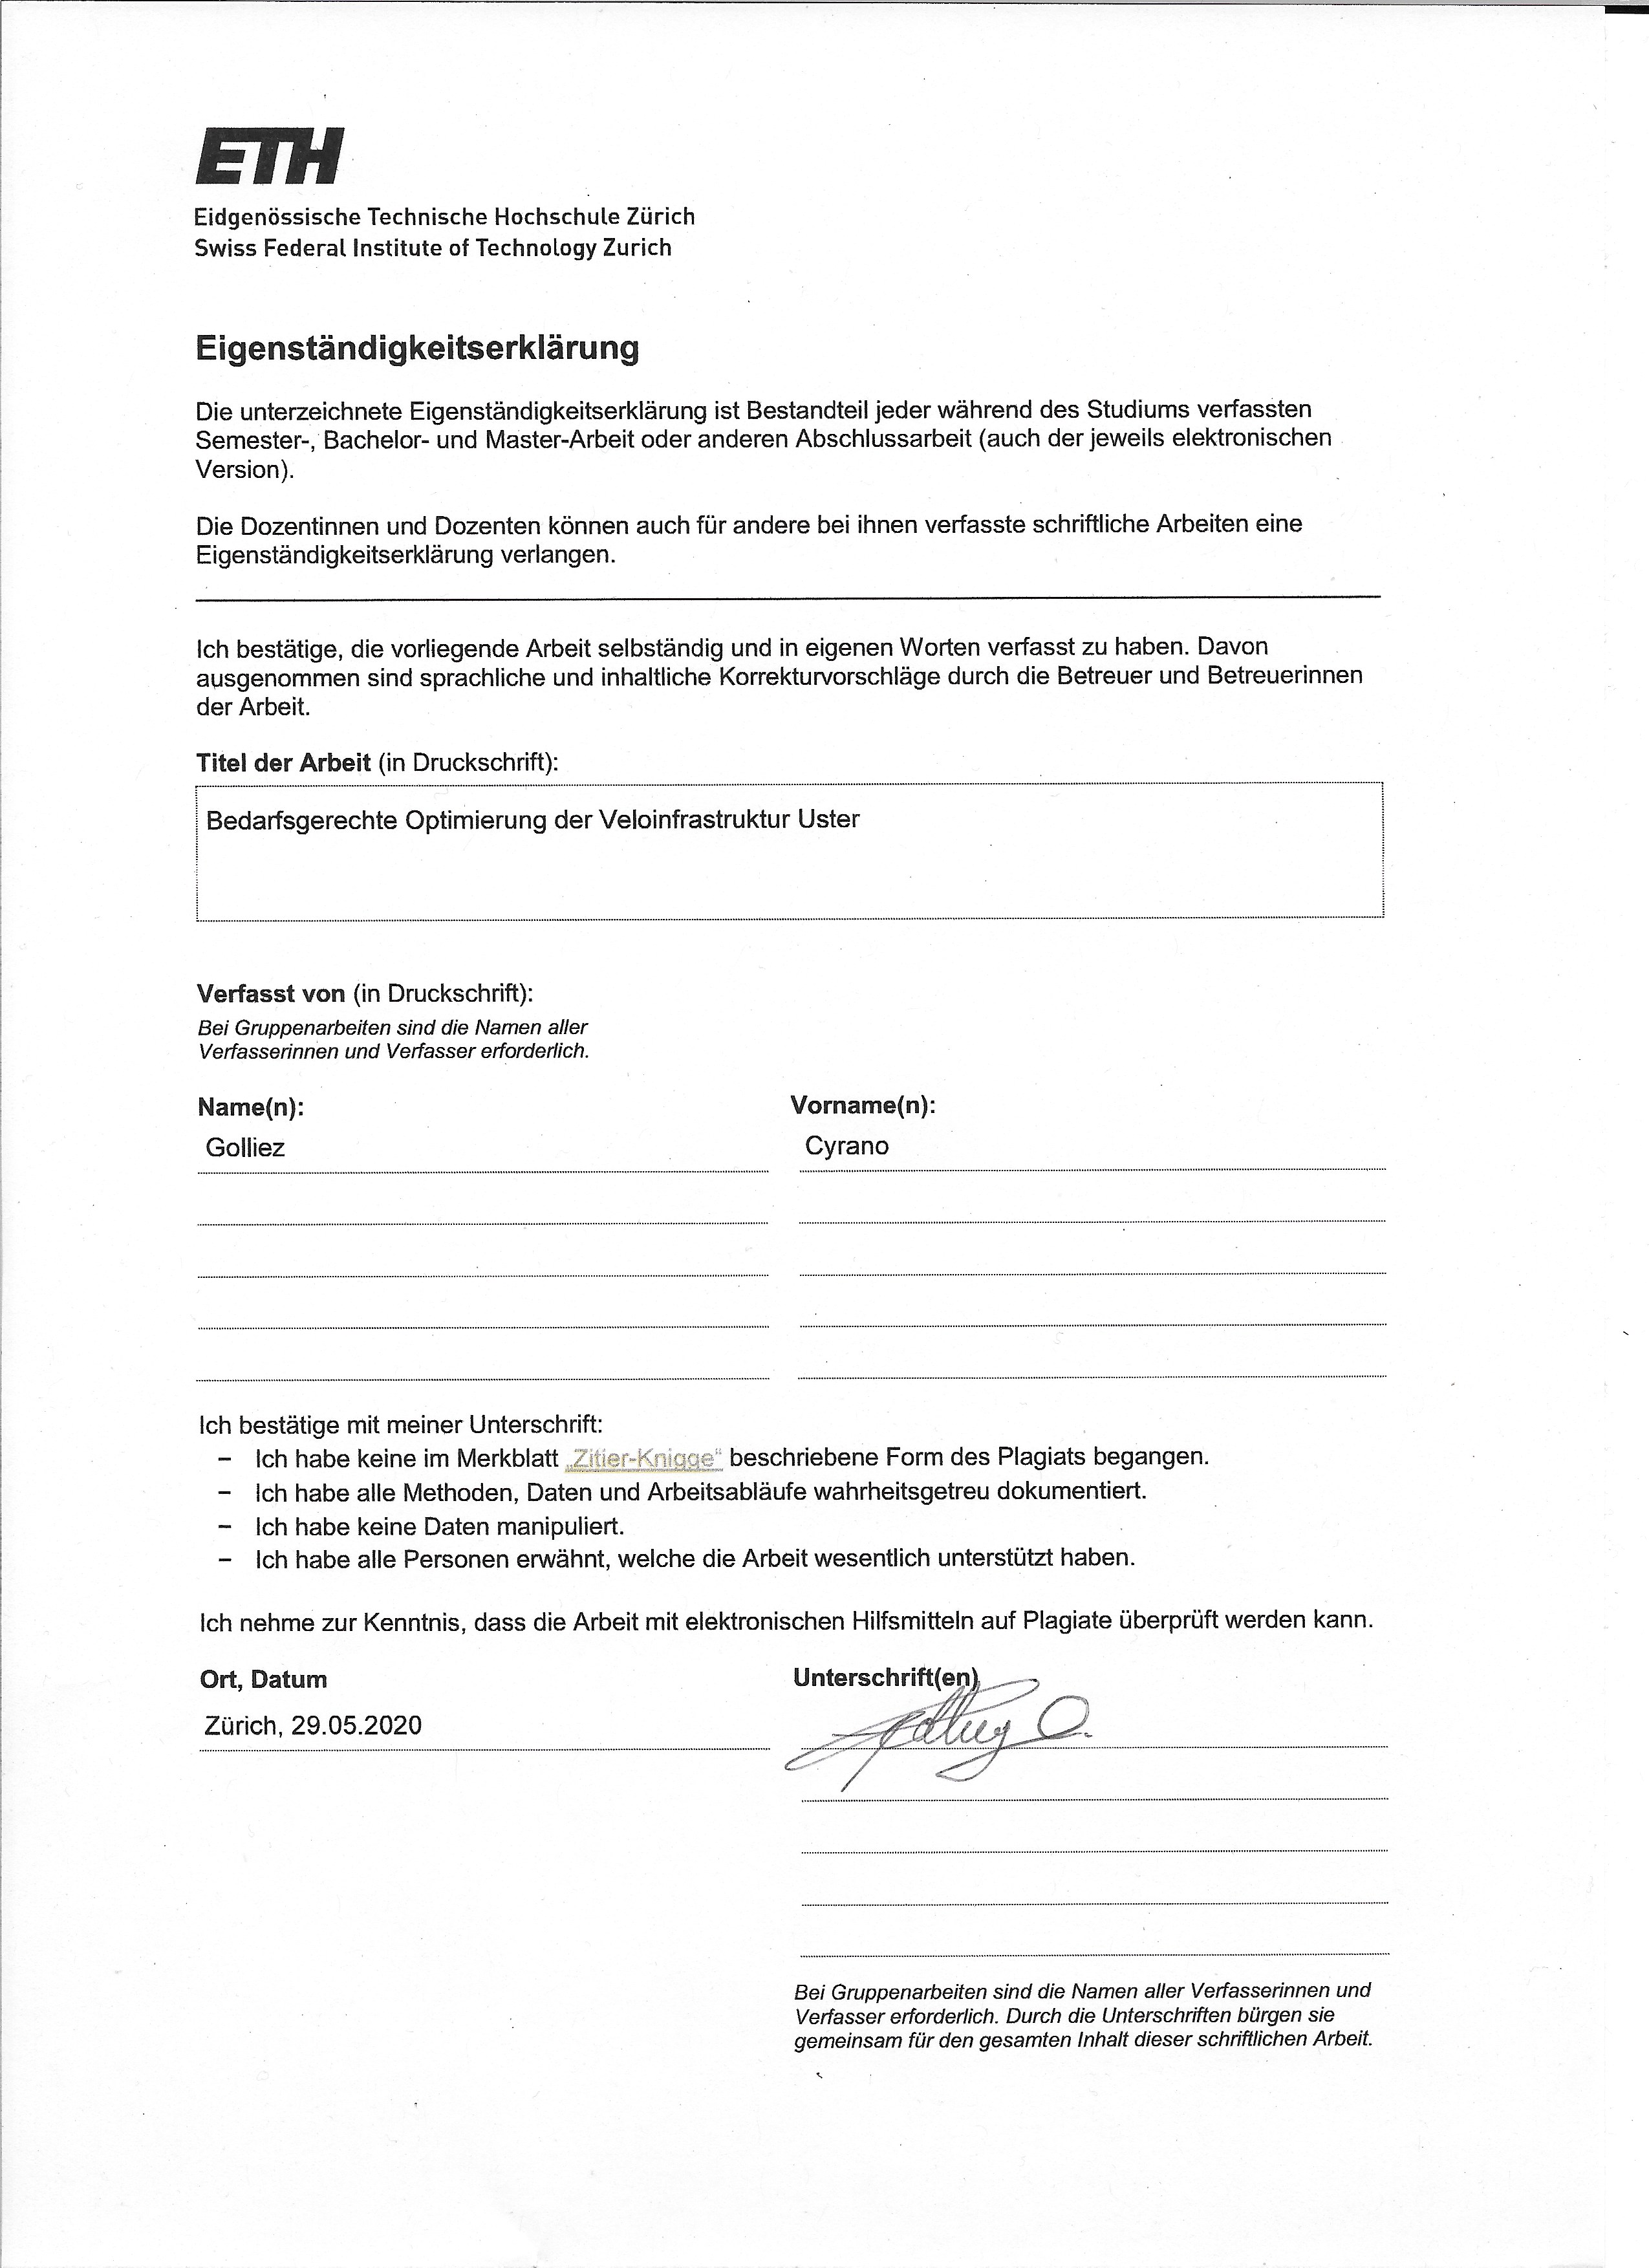
\includegraphics[width=\textwidth]{content/f-00-02-a-Declaration}
\end{figure}


\cleardoublepage

\begin{figure}[h!]
	\centering
	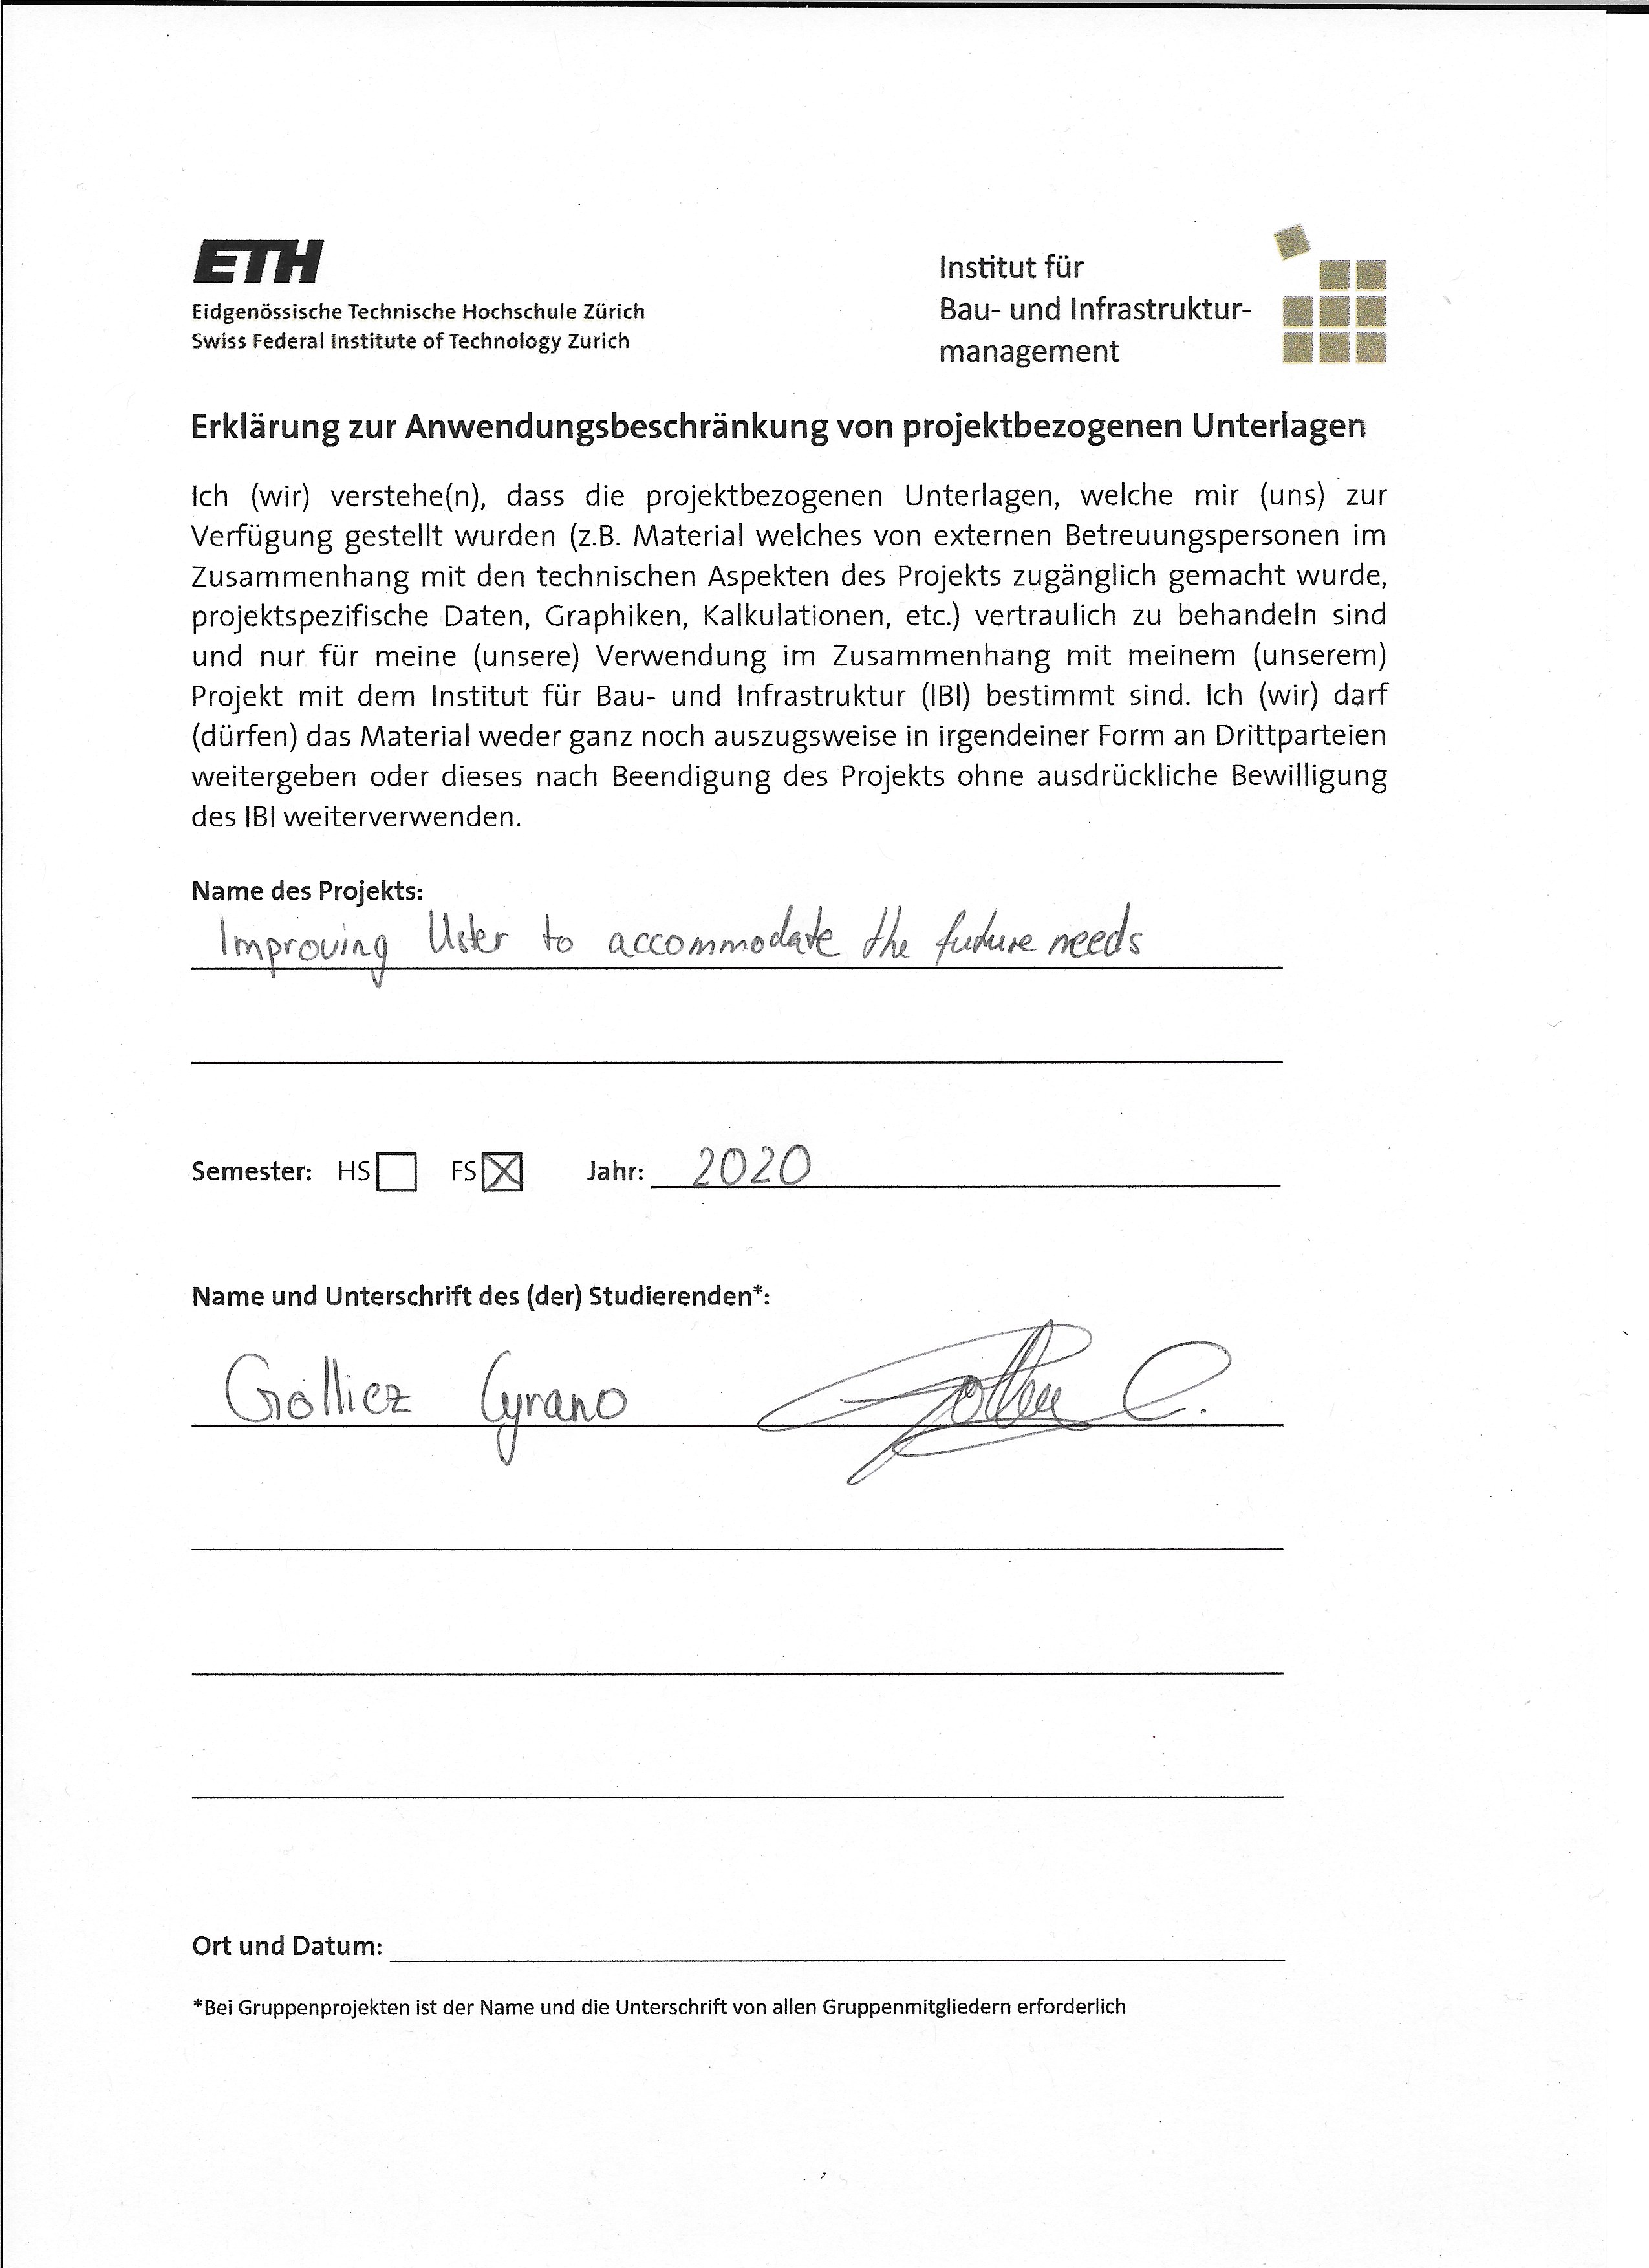
\includegraphics[width=\textwidth]{content/f-00-02-b-Declaration}
\end{figure}

%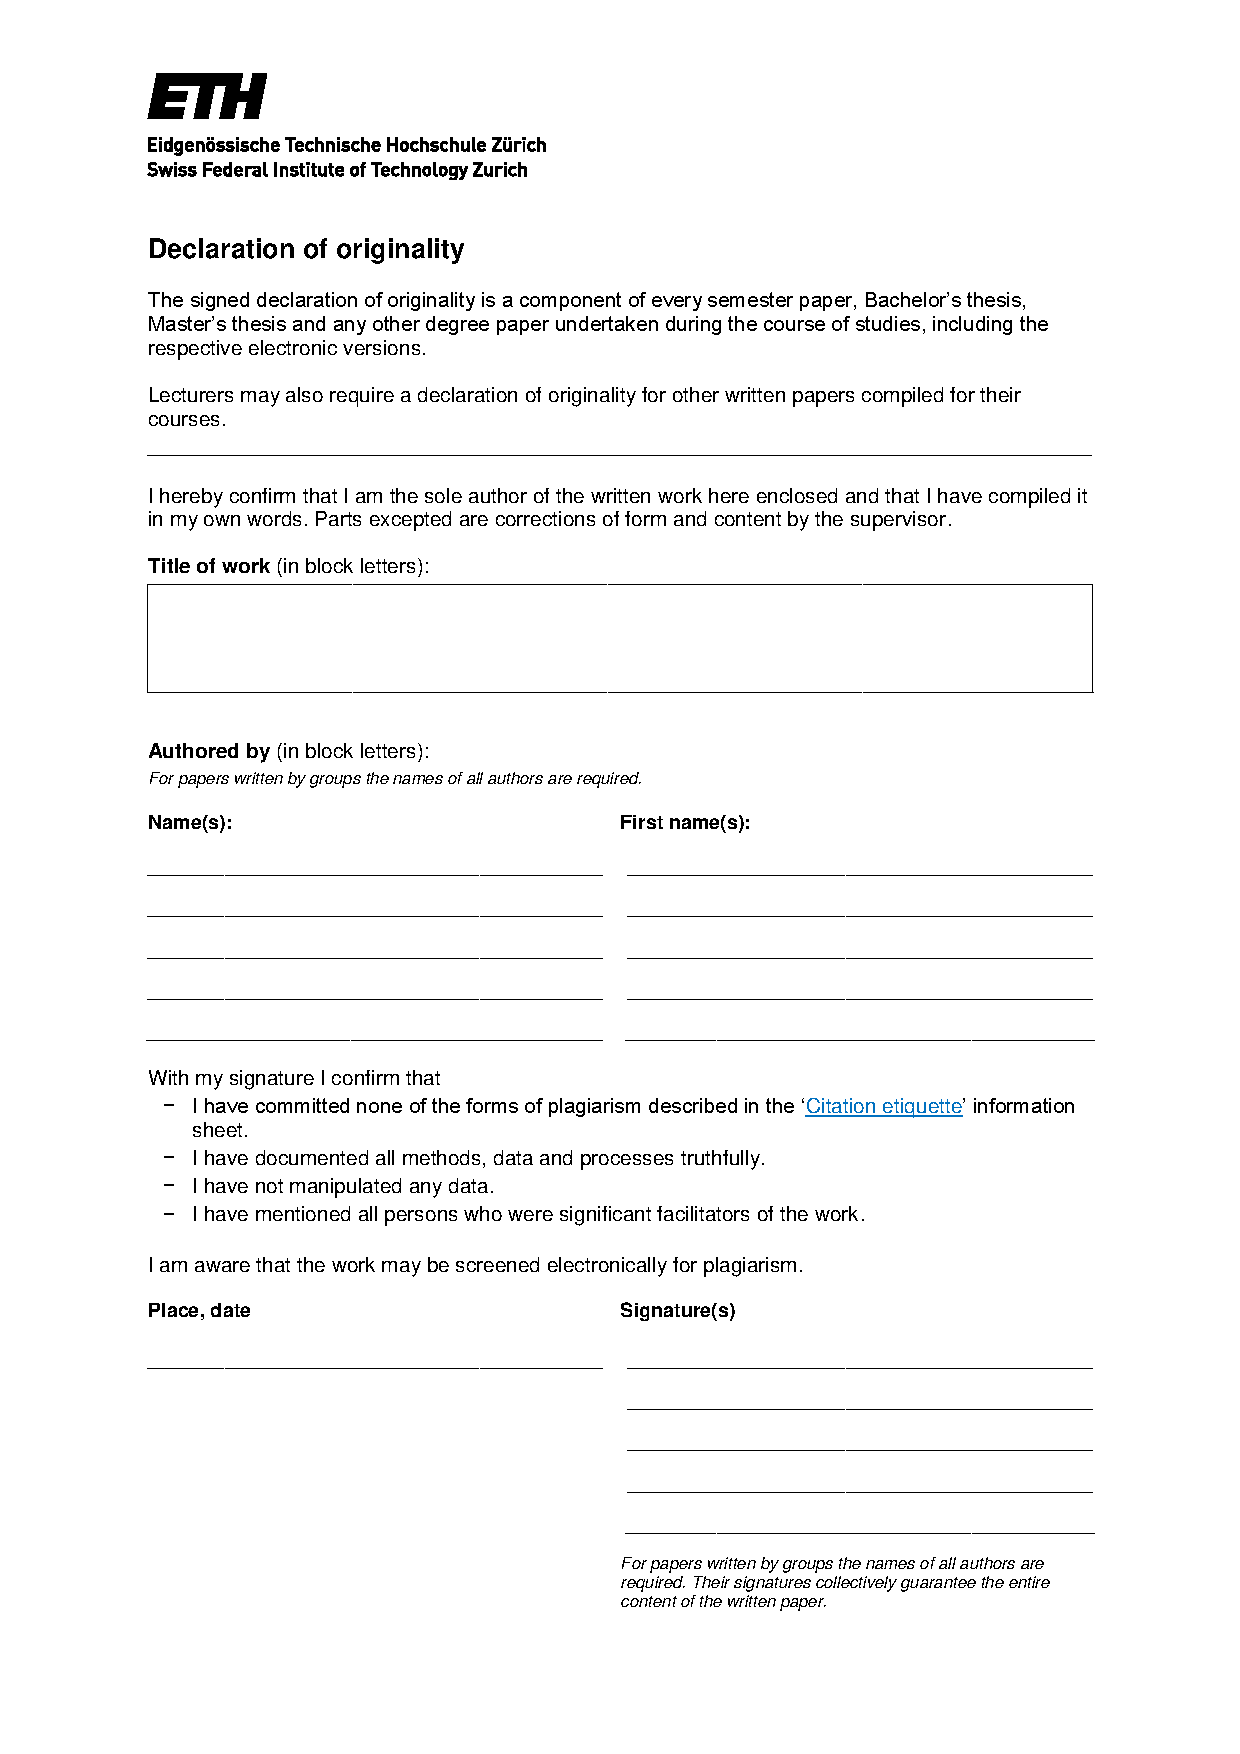
\includepdf[pagecommand={\thispagestyle{empty}},fitpaper=true,pages=-]{content/00-02-a-Declaration}

% Acknowledgment
% --------------
\cleardoublepage
\addcontentsline{toc}{chapter}{Acknowledgment}
%=============================================================================
% Thesis Template in LaTex
%
% File:  00-04-Acknowledgment.tex -- Acknowledgment
% Author(s): Juergen Hackl <hackl@ibi.baug.ethz.ch>
%            Clemens Kielhauser <kielhauser@ibi.baug.ethz.ch>
%
% Creation:  27 Jan 2014
% Time-stamp: <Tue 2013-08-13 20:14 juergen>
%
% Copyright (c) 2014 Infrastructure Management Group (IMG)
%               http://www.ibi.ethz.ch
%
% More information on LaTeX: http://www.latex-project.org/
%=============================================================================

\chapter*{Acknowledgment}
\label{chap:acknowledgment}

An dieser Stelle möchte ich mich bei all denjenigen bedanken, die mich während der Anfertigung dieser Bachelorarbeit unterstützt haben. So möchte ich Prof. Dr. Bryan T. Adey Danken das er mich diese Bachelorarbeit hat durchführen lassen und Herr Dr. Claudio Martani für die grossartige Unterstützung während des gesamten Prozesses meiner Arbeit, die lehrreichen Diskussionen und die aufschlussreichen Rückmeldungen.

% ===========================================================================
% EOF
%

%%% Local Variables:
%%% mode: latex
%%% TeX-master: "../main"
%%% End:

% Abstract
% --------
\cleardoublepage
\addcontentsline{toc}{chapter}{Abstract}
%=============================================================================
% Thesis Template in LaTex
%
% File:  00-03-Abstract.tex -- Abstract of the Thesis
% Author(s): Juergen Hackl <hackl@ibi.baug.ethz.ch>
%            Clemens Kielhauser <kielhauser@ibi.baug.ethz.ch>
%
% Creation:  27 Jan 2014
% Time-stamp: <Tue 2013-08-13 20:14 juergen>
%
% Copyright (c) 2014 Infrastructure Management Group (IMG)
%               http://www.ibi.ethz.ch
%
% More information on LaTeX: http://www.latex-project.org/
%=============================================================================

\chapter*{Abstract}
\label{chap:abstract}

look at \ref{chap:abstract}

The abstract is a concise and accurate summary of the research described in the document. It states the problem, the methods of investigation, and the general conclusions, and should not contain tables, graphs, complex equations, or illustrations. There is a single abstract for the entire work, and it must not exceed 350 words in length.

The abstract should be given in both English and German language, independent of the language in which the thesis itself is written.



%=============================================================================
% EOF
%

%%% Local Variables:
%%% mode: latex
%%% TeX-master: "../main"
%%% End:


% Zusammenfassung
% --------
\cleardoublepage
\addcontentsline{toc}{chapter}{Zusammenfassung}
%=============================================================================
% Thesis Template in LaTex
%
% File:  00-05-Zusammenfassung.tex -- Zusammenfassung der Thesis
% Author(s): Juergen Hackl <hackl@ibi.baug.ethz.ch>
%            Clemens Kielhauser <kielhauser@ibi.baug.ethz.ch>
%
% Creation:  27 Jan 2014
% Time-stamp: <Tue 2013-08-13 20:14 juergen>
%
% Copyright (c) 2014 Infrastructure Management Group (IMG)
%               http://www.ibi.ethz.ch
%
% More information on LaTeX: http://www.latex-project.org/
%=============================================================================

\chapter*{Zusammenfassung}
\label{chap:Zusammen}

Das Ziel dieser Arbeit war die Optimierung des Verkehrssystems von Uster durch Verbesserung eines Teilstücks der Veloinfrastruktur. Dazu wurde die Infrastruktur des Bahnübergangs
Brunnenstrasse in Abhängigkeit von unsicheren zukünftigen Nachfragebeziehung untersucht und verschiedene Vorschläge zur Verbesserung der Situation erarbeitet. Daraus wurde eine optimale Variante abgeleitet, welche die zukünftigen Bedürfnisse der Bevölkerung von Uster nach Mobilität am besten befriedigen kann.

Die Optimierung bestehender Infrastruktursystem stellt eine der grossen Herausforderungen des Infrastruktur Management dar. So ist in den meisten Fällen einerseits nicht eindeutig zu bestimmen, was genau die Probleme sind und durch was sie verursacht werden. Andererseits ist nicht immer vollständig festgelegt, was mit einer Veränderung erreicht werden soll. Hinzu kommt, dass nicht immer ersichtlich ist, welche Varianten einer Optimierung überhaupt möglich sind und welche unter Berücksichtigung unsicherer zukünftiger Entwicklungen der Kosten und Nutzen der Beteiligten optimal ist.

Die Bedürfnisse und Anforderungen der Nutzer und Besitzer der Infrastruktur können sich während der Lebensdauer drastisch verändern. Die Schwierigkeit ist daher, Infrastrukturen so zu gestalten, dass sie über ihre gesamte Lebensdauer ein angemessenes Leistungsniveau gewährleisten können. Es ist von allgemeinem Interesse, dass eine Intervention in eine bestehende Infrastruktur nur dann durchgeführt wird, wenn der Netto-Nutzen aller Beteiligten maximiert wird.

Im Rahmen dieser Projektarbeit habe ich für die bestehende Verkehrsproblematik von Uster verschiedene Varianten erarbeitet und eine optimale Lösung bestimmt. Dabei habe ich mich auf den Problemlösungsprozess aus dem Kurs Systems Engineering sowie auf die Theorie der Zielfunktion, des Entscheidungsbaumes und der Sensitivitätsanalysen gestützt. Um die Unsicherheiten zukünftiger Entwicklungen in den Entscheidungsprozess einfliessen zu lassen, wurden die entsprechenden Einflussfaktoren anhand von Prognosen geschätzt. Anschliessend wurde der Einfluss verschiedener Parametervariationen auf die Kostenberechnung modelliert und die ermittelten Werte mit der geschätzten Eintrittswahrscheinlichkeit der Szenarien gewichtet. Auf dieser Basis wurden die zur Auswahl stehenden Varianten beurteilt. Dabei hat sich die Variante 2 als die beste Option für die Zukunft von Uster herausgestellt.



%=============================================================================
% EOF
%

%%% Local Variables:
%%% mode: latex
%%% TeX-master: "../main"
%%% End:


% Hilfestellung Template
% ----------------------
%\cleardoublepage
%\addcontentsline{toc}{chapter}{Hilfestellung}
%%=============================================================================
% Thesis Template in LaTex
%
% File:  1-Introduction.tex -- Introduction to the topic
% Author(s): Jürgen Hackl <hackl@ibi.baug.ethz.ch>
%            Clemens Kielhauser <kielhauser@ibi.baug.ethz.ch>
%
% Creation:  27 Jan 2014
% Time-stamp: <Tue 2013-08-13 20:14 juergen>
%
% Copyright (c) 2014 Infrastructure Management Group (IMG)
%               http://ibi.ethz.ch
%
% More information on LaTeX: http://www.latex-project.org/
%=============================================================================

\chapter*{Hilfestellung}
\label{chap:Hilfe}

\section*{Some formal aspects}
\label{sec:formalaspects}

Strong demands can only be met with the help of a very stringent and clear structure laid out at the beginning of the writing process. One of the most clear structuring is given by a rigorous "legal numbering" (1, 1.1, 1.1.1 etc.). It is good to know that \LaTeX does all this formatting business without any need to renumber things yourself at each iteration and so on. Thus we strongly recommend using \LaTeX for the project. Anything else (e.g. Word) is a mess when writing an elaborate scientific text with many graphics and formulas.

Even a particular elusive reader should be able to quickly glean the most important thoughts, experiments and results from just looking at illustrative schematics, diagrams, and pictures with self explaining, extensive figure captions.

There are always parts/chapters/sections of text which are complex and important for a full description and documentation of the work, but not absolutely necessary for following the main lines of thought. It is very helpful for the somewhat more interested, but temporally limited reader if such passages of text are correspondingly marked, e.g. by a brief introductory remark to such sections, or even by moving them into appendices.

Definitively each chapter and ideally also each section should begin with a short guide: what is communicated in the following text, which sources (quote clearly) have been used, what are the basic concepts used and which goals are to be reached. Similarly, at the end of larger elaborations a short synopsis of the communicated content should be
offered.

\subsection*{Plain text}
\label{sec:plaintext}

A single font must be used throughout the thesis or report, the only exceptions being in tables, graphs, and appendices. Headings may be bolded and no more than 2 points larger than the rest of the text.

The page format should be single column with one and a single spacing used
between the lines. Spacing of words on a line should be such that the line can be easily read. Crowding words together or leaving excessive spaces is not permitted.

\subsection*{Footnotes}
\label{sec:footnotes}


For those who are using footnotes\footnote{Some example footnote.}, Arabic numerals are used consecutively throughout a chapter, and should normally appear at the bottom of the relevant page, keyed to the same number following the word or phrase in the text to which it refers. If a footnote is too long for the relevant page, it may be continued on the following page preceding the footnotes for that page. If the number of footnotes is very large, numbers may be restarted with each chapter.


\subsection*{Lists}
\label{sec:lists}

There are three types of lists with the environment names \emph{itemize}, \emph{enumerate} and \emph{description}. All lists have a separation between each item, to improve the reading of item texts spanning several lines. This item text can contain multiple paragraphs. These paragraphs are appropriately spaced and indented according to their position in the list. 

\begin{itemize}
\item 
The \emph{itemize} sets off list items with \emph{bullets}, like this.
%
\item Of course, lists can be nested, each type up to at least four levels.
One type of list can be nested within another type.
%
  \begin{itemize}
  \item Nested lists of the same type will change style of numbering 
  or \emph{bullets} as needed.
  \end{itemize}
\end{itemize}
%
\begin{enumerate}
\item The \emph{enumerate} environment numbers the list elements.

This is a new paragraph in the item text, which is not intended as in the normal text but separated from the previous paragraph.
%
\item The enumeration scheme changes with each nesting level
  \begin{enumerate}
  \item as shown in this nested enumerated list item.
  \end{enumerate}
\end{enumerate} 

\begin{description}
\item[Some description] The \emph{description} environment allows to describe some content.
\end{description}

\subsection*{Mathematical symbols and equations}
\label{sec:math}

Each formula, except for generally accepted and well-known formulas, either has to be mathematically derived, to be explained, or a literature source has to be provided. This applies especially to complex models, where each constraint should be described and explained.

There are three types of mathematical equations: (a) in-line equations, (b) displayed butunnumbered equations, and (c) displayed and numbered equations.

\subsubsection*{In-line equations}
\label{sec:inlineeq}

An in-line equation is used for particularly simple relationships which (i) do not need vertical space for integrals, fractions, etc., (ii) can be expressed without breaking the flow of the sentence, and (iii) will not be referenced again in the document.

For example:

\begin{IMleftrightskip}
If volume $V$ and temperature $T$ are known, the ideal gas law can be used to get a reasonable approximation for the pressure of a gas as $P=nRT/V$, where $n$ is the number of moles of gas and $R$ is the gas constant.
\end{IMleftrightskip}

Unless all the variables have been defined earlier in the document, the physical significance of all the quantitie s appearing in an equation must be stated at the point of their first appearance in the document.

\subsubsection*{Displayed, but unnumbered, equations}
\label{sec:diuneq}

Equations that are too complex to be written as in-line equations should be "displayed", which usually means, that the equation is centered between the left and right margins or aligned at a tab stop
with some indent from the left margin and some vertical space is provided above and below the equation to set it apart from the text.

For example:


\begin{IMleftrightskip}
The van der Waals equation is used to provide a more accurate expression for the pressure $P$ as a function of the molar volume $V_m$ and the temperature $T$ as
%
\begin{equation*}
P = \frac{RT}{V_m-b}-\frac{a}{V_m^2}~,
\end{equation*}
%
where $a$ and $b$ are van der Waals parameters for the gas.

or

The electric field $\mathbf{E}$ at the origin due to a point charge $q$ at a distance $r$ is given by
%
\begin{equation*}
\mathbf{E} = \frac{|q|}{4\pi\varepsilon_0 r^2}\mathbf{\hat{r}}
\end{equation*}
where $\mathbf{\hat{r}}$ is the position vector of the point charge.
\end{IMleftrightskip}

Note that in the examples presented above, the displayed equation is part of the text, i.e, it is punctuated, and incorporated in to the structure of the sentence.

All the scalar variables are italicized whereas the vector quantities in the second example are Roman boldfaced.

\subsubsection*{Displayed and numbered equations}
\label{sec:dineq}

One often has to refer back to the important equations. The standard way to do this is by referring to the equation number. Of course, in order to refer to an equation number, one must first number the equations. A consiste nt system of numberi ng equations must be adopted. Various options are:
\begin{itemize}
\item Number equations as (1), (2), etc., starting in Chapter 1 (or at the first numbered equation) and continuing until the end of the last numbered equation in the document.
\item Incorporate the chapter number into the equation, as in (1.1),  (2.3), (4.6), etc., which means the equation numbering goes back to 1 at the beginning of each chapter.
\item Use Roman numerals for chapter numbers, as in (I.1), (II.3), (IV.6) etc.
\end{itemize}

For example:

\begin{IMleftrightskip}
The non-relativistic Schrödinger equation for a particle of mass m
subject to a potential energy function V(x) in a one-dimensional universe is
%
\begin{equation}
  \label{eq:1}
  E \psi(x) = \frac{-\hbar^2}{2m} \frac{d^2\psi}{d x^2} + V(x)\psi(x)
\end{equation}
%
where $\hbar = h/(2\pi)$, $h$ is Plack’s constant, and $E$ is the total energy of the system.
\end{IMleftrightskip}

The equation in the example is approximately centered on the page, and the equation number is aligned by a right-tab at the right margin.

To cite an equation in text, use an abbreviation if it is not the first word of the sentence. Suitable singular and plural ab breviations include eq. and eqs., Eq. and Eqs. Spell out “Equation” when it is the first word of a sentence and when it is not accompanied by a number.

The used numbering of the equation may change according to the context of the work. E.g. number them as subequations
\begin{subequations}
\begin{align}
  \dot{q}_i & = \frac{\partial H}{\partial p_i} \\
  \dot{p}_i & = -\frac{\partial H}{\partial q_i} 
\end{align}
\end{subequations}
or with only a single number
\begin{equation}
\begin{aligned}
  \dot{q}_i & = \frac{\partial H}{\partial p_i} \\
  \dot{p}_i & = -\frac{\partial H}{\partial q_i} 
\end{aligned}
\end{equation}
Many further possibilities of displaying equations exist.

%\subsection{Theorems}
%\label{sec:theorems}

\subsection*{Tables}
\label{sec:tables}

Tables should only be used to present three (3) or more items; otherwise, the data should be described in the narrative. Tables should be arranged so like material appears in columns, not rows. Information presented in tables should be sufficiently understandable so frequent reference to the narrative is unnecessary. Each table should have a title, generally appearing above the table itself. The table title and other items may be footnoted, although extensive explanations appearing in footnotes should be avoided. All abbreviations and symbols should be defined.

Tables are generally no more than what can be printed on one page, but occasionally multi-paged tables are necessary and are acceptable. Tables may appear on pages which contain narrative text or tables may appear singularly on a page (i.e. one table per page and only the table on the page).

%=============================================================================
% Thesis Template in LaTex
%
% File:  t-05-01-IsingModel.tex -- Table for the Ising
% Author(s): Juergen Hackl <hackl@ibi.baug.ethz.ch>
%            Clemens Kielhauser <kielhauser@ibi.baug.ethz.ch>
%
% Creation:  27 Jan 2014
% Time-stamp: <Tue 2013-08-13 20:14 juergen>
%
% Copyright (c) 2014 Infrastructure Management Group (IMG)
%               http://ibi.ethz.ch
%
% More information on LaTeX: http://www.latex-project.org/
%=============================================================================

\begin{table}[ht]
\centering
\small\renewcommand{\arraystretch}{1.2}  
%
\captionabove[Mean-field predictions for the critical temperature of the Ising model]{Comparison of the mean-field predictions for the critical temperature of the Ising model with exact results and the best known estimates for different spatial dimensions $d$ and lattice symmetries.}
\label{tab:t-03-01-IsingModel}
%
\begin{tabularx}{0.5\textwidth}{lXXX}
\toprule
\textbf{lattice} & $d$ & $q$ & $T_\text{mf}/T_c$ \\
\hline
square  & 2 & 4 & 1.763 \\
%
triangular & 2 & 6 & 1.648 \\
%
diamond & 3 & 4 & 1.479 \\
%
simple cubic & 3 & 6 & 1.330 \\
%
bcc & 3 & 8 & 1.260 \\
%
fcc & 3 & 12 & 1.225 \\
\hline
\end{tabularx}
\end{table}

%=============================================================================
% EOF
%

%%% Local Variables:
%%% mode: latex
%%% TeX-master: "../guidelines"
%%% End:


\subsection*{Figures}
\label{sec:figures}

Figures present charts, graphs, or images to the reader. Figure legends should be sufficiently detailed to allow the reader to understand without frequent reference to the narrative. However, overly detailed descriptions should be avoided. All abbreviations and symbols should be defined. Figure legends should appear on the same page and in the same orientation as the figure. For example, if the figure appears in landscape mode then the legend should also appear in landscape mode. If the figure legend is too lengthy to appear on the same page as the figure, then the legend, in its entirety, must appear on the next page.

Similar to tables, figures are usually constructed to be no more than what can appear on one page, but occasionally multi-paged figures are necessary. Figures may also appear singularly on pages or on pages containing narrative text.


\begin{figure}[h!]
  \centering
  %=============================================================================
% Thesis Template in LaTex
%
% File:  f-01-01-a-R-S.tex -- Classical Approach R-S
% Author(s): Jürgen Hackl <hackl@ibi.baug.ethz.ch>
%            Clemens Kielhauser <kielhauser@ibi.baug.ethz.ch>
%
% Creation:  27 Jan 2014
% Time-stamp: <Tue 2013-08-13 20:14 juergen>
%
% Copyright (c) 2014 Infrastructure Management Group (IMG)
%               http://ibi.ethz.ch
%
% More information on LaTeX: http://www.latex-project.org/
%=============================================================================

% ******
% Figure
% ******

% Document name
% =============

% f-00-00-a-Example.txt

% f  ... Figure
% 00 ... Chapter
% 00 ... Number of the figure
% a  ... Subfigure
% Ex ... Name of the figure


% Libraries
% =========

\usetikzlibrary{shapes,arrows}
\usetikzlibrary{positioning}
\usetikzlibrary{shadows}
\usetikzlibrary{backgrounds}
% \usepackage{verbatim}
\usetikzlibrary{automata}
\usetikzlibrary{arrows}
\usetikzlibrary{calc}
\usetikzlibrary{patterns}



% Styles
% ======

% Line Width
% ----------

\tikzstyle{hugeLine}=[line width=1.7pt]
\tikzstyle{bigLine}=[line width=1.3pt]
\tikzstyle{normalLine}=[line width=1pt]
\tikzstyle{smallLine}=[line width=.7pt]
\tikzstyle{tinyLine}=[line width=.5pt]

% Line Types
% ----------

\tikzstyle{Axis}=[smallLine,-to]
\tikzstyle{Line}=[normalLine]
\tikzstyle{Solid}=[fill=black!10]
\tikzstyle{Arrow}=[>=latex,smallLine,->]
\tikzstyle{Dimension}=[tinyLine,|-|]


% TikZ figure
% ===========

\begin{tikzpicture}


  % Grid
  % ----

  % \node [coordinate](ValA) at (0,0) {};
  % \node [coordinate](ValB) at (8,4) {};
  % \fill [fill=white](ValA) circle (.1pt);
  % \fill [fill=white](ValB) circle (.1pt);
  % \draw[help lines,step=1cm] (ValA) grid (ValB);

  \footnotesize

  % Distribution R
  \begin{scope}[xshift=4.5cm,yshift=0cm]
    \draw[tinyLine,dashed](0,0)--++(0,3) node [below,pos=0]{$\mu_R$};
    \draw[Dimension](0,1.95)--++(.46,0) node [below,pos=.6]{$\sigma_R$};
    \draw[Line,domain=-1.5:1.5,scale=1.5,smooth] plot (\x,{2*exp(-(\x)*(\x)*0.5/0.1)});
  \end{scope}

  \begin{scope}[xshift=2.9cm,yshift=0cm]
    \draw[tinyLine,dashed](0,0)--++(0,2) node [below,pos=0]{$\mu_S$};
    \draw[Dimension](0,1.1)--++(-.6,0) node [below,pos=.5]{$\sigma_S$};
  \draw[Line,domain=-2:2,scale=1,smooth] plot (\x,{2*exp(-(\x)*(\x)*0.5/0.3)});
  \end{scope}



  % \end{scope}

  % Axis
  \draw [Axis] (0,-.3)--(0,3) node [left, pos=1] {$f_S(s)$} node [left, pos=.85] {$f_R(r)$};
  \draw [Axis] (-.3,0)--(8,0) node [below, pos=.98] {$r,s$};

  % Comment
  \node (S) at (2.2,1.7){$S$};
  \node (R) at (5.2,2.6){$R$};
  \begin{scope}[xshift=0cm,yshift=-1.8cm]
  \begin{scope}[xshift=1.6cm,yshift=0cm]
    \fill[Solid,domain=-4.5:4.5,scale=.5,smooth] plot (\x,{2*exp(-(\x)*(\x)*0.5/2.5)});
    \fill[white](-1.6,0) rectangle (3.5,1);
    \draw[tinyLine,dashed](0,0)--++(0,1) node [below,pos=0]{$\mu_M$};
    \draw[Dimension](0,.7)--++(-.7,0) node [below,pos=.5]{$\sigma_M$};
    \draw[Line,domain=-4.5:4.5,scale=.5,smooth] plot (\x,{2*exp(-(\x)*(\x)*0.5/2.5)});
  \end{scope}

  % Dimension
  \draw[Dimension](0,-.5)--++(1.6,0) node [below,pos=.5]{$\beta\cdot \sigma_M$};

  % Arrow
  \draw [Arrow](-.3,.3)--(-.1,.05)node [left=0,pos=.0]{$p_f$};

  % Axis
  \draw [Axis] (0,-.3)--(0,1) node [left, pos=1] {$f_M(m)$};
  \draw [Axis] (-.3,0)--(8,0) node [below, pos=.99] {$m$};

  % Comment
  \node (M) at (2.6,.8){$M$};
  \end{scope}

  % Dimension
  \draw[Dimension](2.9,-.5)--(4.5,-.5) node [below,pos=.5]{$\beta\cdot \sigma_M$};

\end{tikzpicture}



% ===========================================================================
% EOF
%

%%% Local Variables:
%%% mode: latex
%%% TeX-master: "../main"
%%% End:

  \caption[Safety Margin an Reliability Index]{Safety Margin an Reliability Index. Are the random variables $R$ and $S$ normally distributed also the safety margin $M$ is a normal random variable. In standardised domain the reliability index $\beta$ provides the information how often $\sigma_{{M}}$ has space between the origin and $\mu_{{M}}$.}
  \label{fig:f-01-01-a-SafetyMargin}
\end{figure}

All possibilities of grouping pictures side by side, on top or in matrices can be realized. Each subfigure is created in the same way  as a graphic inside a figure, just enclosed by a figure environment, as shown in Figure \ref{fig:f-01-02-FORM}.


\begin{figure}[h!]
  \centering
  \subfloat[][]{\label{fig:f-01-02-a}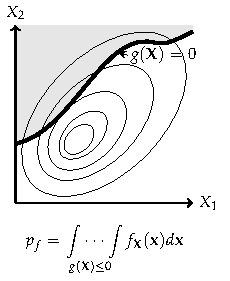
\includegraphics[width=.32\textwidth]{./figures/f-01-02-a-FORM}}
  \hfill
  \subfloat[][]{\label{fig:f-01-02-b}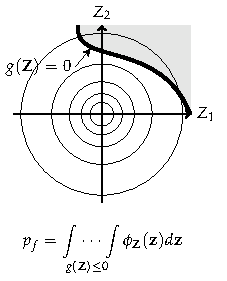
\includegraphics[width=.32\textwidth]{./figures/f-01-02-b-FORM}}
  \hfill
  \subfloat[][]{\label{fig:f-01-02-c}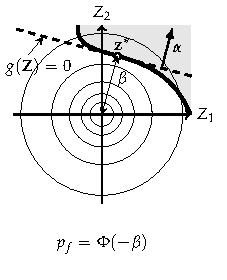
\includegraphics[width=.32\textwidth]{./figures/f-01-02-c-FORM}}
\caption[First Order Reliability Method]{First Order Reliability Method. (a) Representation of a physical space with a set $\mathbf{X}$ of any two random variables. The shaded area denotes the failure domain and $g(\mathbf{X})=0$ the failure surface. (b) After transformation in the normalized space, the random variables $\mathbf{Z}$ are now uncorrelated and standardized normally distributed, also the failure surface is transformed into $g(\mathbf{X})=0$. (c) FORM corresponds to a linearization of the failure surface $g(\mathbf{X})=0$. Performing this method, the design point $\mathbf{z}^*$ and the reliability index $\beta$ can be computed.}
  \label{fig:f-01-02-FORM}
\end{figure}

\subsection*{Citations}
\label{sec:citations}

Academic work almost always builds upon the work of others, and it is appropriate, indeed essential, that you discuss the related and previous work of others in your thesis. However, this must be done according to the rules of acceptable use.

Much of the advice in the section on books will pertain to other sources as well. Their long history as a formal publication ensures, in particular, that the variations in author names and titles will serve as a model for constructing documentary notes and bibliography entries for many other types of sources.

The Chicago Manual of Style\footnote{\cite{chicago2010}}, implemented here in its 16th edition, has long, been one of the most influential style guides for writers and publishers. While one’s choices are now perhaps more extensive than ever, the Manual at least still provides a widely-recognized, and widely-utilized, standard.

A full reference must include enough information to enable an interested reader to locate the book. Most references contain at least some information not strictly needed for that purpose but potentially helpful nonetheless. The elements listed below are included, where applicable, in full documentary notes and bibliography entries.

%\begin{refsection}
The author appears as part of the narrative:
\begin{IMleftrightskip}
 \cite[p.100]{Nowak2000} show how to calculate the reliability index $\beta$, by using geometric properties.
 And \cite{chicago2010} shwos us how to eat ass.
\end{IMleftrightskip}

Otherwise, in parentheses:
\begin{IMleftrightskip}
A near linear relationship can be obtained between ultimate flexural and shear capacity of a RC section, if pitting corrosion occurs \footcite{Stewart2009}.


\cite[vlg.][17]{Nowak2000} Das ist mit Seitenangabe und Vergleich

\cite{Nowak2000} Das ist sogar sehr doof. 

\autocite{Nowak2000} Das ist ein Test.
\end{IMleftrightskip}
%\printbibliography[heading=none]
%\end{refsection}

% ===========================================================================
% EOF
%

%%% Local Variables:
%%% mode: latex
%%% TeX-master: "../main"
%%% End:
 

% Table of Contents
% -----------------
\cleardoublepage
\tableofcontents

% List of Figures
% ---------------
\cleardoublepage
\listoffigures

% List of Tables
% --------------
\cleardoublepage
\listoftables

% Nomeclature
% -----------
%\addcontentsline{toc}{chapter}{Nomeclature}

% Glossary
% --------
%\addcontentsline{toc}{chapter}{Glossary}

%\cleardoublepage
%\printglossary[type=main]

\cleardoublepage
\addcontentsline{toc}{chapter}{Glossary}
%=============================================================================
% Thesis Template in LaTex
%
% File:  00-04-Acknowledgment.tex -- Acknowledgment
% Author(s): Juergen Hackl <hackl@ibi.baug.ethz.ch>
%            Clemens Kielhauser <kielhauser@ibi.baug.ethz.ch>
%
% Creation:  27 Jan 2014
% Time-stamp: <Tue 2013-08-13 20:14 juergen>
%
% Copyright (c) 2014 Infrastructure Management Group (IMG)
%               http://www.ibi.ethz.ch
%
% More information on LaTeX: http://www.latex-project.org/
%=============================================================================

\chapter*{Glossar}
\label{chap:Glossar}

%=============================================================================
% Thesis Template in LaTex
%
% File:  t-05-01-IsingModel.tex -- Table for the Ising
% Author(s): Juergen Hackl <hackl@ibi.baug.ethz.ch>
%            Clemens Kielhauser <kielhauser@ibi.baug.ethz.ch>
%
% Creation:  27 Jan 2014
% Time-stamp: <Tue 2013-08-13 20:14 juergen>
%
% Copyright (c) 2014 Infrastructure Management Group (IMG)
%               http://ibi.ethz.ch
%
% More information on LaTeX: http://www.latex-project.org/
%=============================================================================

\begin{longtable}[c]{ll}
%\center
%\renewcommand{\arraystretch}{1.4}
\toprule 
Begriff		        & \multicolumn{1}{c}{Definition}        \\ 
\midrule
STEK				& Stadtentwicklungskonzept   \\
DTV                 & Tägliches Verkehrsaufkommen    \\
MIV					& Motorisierter Individualverkehr       \\ 
ÖV					& Öffentlicher Verkehr \\

\label{tab:Glossary}
\end{longtable}




%=============================================================================
% EOF
%

%%% Local Variables:
%%% mode: latex
%%% TeX-master: "../guidelines"
%%% End:




% ===========================================================================
% EOF
%

%%% Local Variables:
%%% mode: latex
%%% TeX-master: "../main"
%%% End:


% arabic page numbers
% ------------------
% \mainmatter
\cleardoublepage
\pagenumbering{arabic}% \setcounter{page}{0}

% Chapter 1
% ---------
%=============================================================================
% Thesis Template in LaTex
%
% File:  01-Einleitung.tex -- Einleitung
% Author(s): Cyrano Golliez <golliezc@student.ethz.ch>
%            
%
% Creation:  27 Jan 2014
% Time-stamp: <Tue 2013-08-13 20:14 juergen>
%
% Copyright (c) 2014 Infrastructure Management Group (IMG)
%               http://ibi.ethz.ch
%
% More information on LaTeX: http://www.latex-project.org/
%=============================================================================

\chapter{Einleitung}
\label{chap:Einleitung}

Im Rahmen dieser Bachelorarbeit im Bereich Infrastruktur Management habe ich, anhand der Verkehrsproblematik von Uster die Anwendung geeigneter Verfahren und Methoden zur Erarbeitung kreativer Lösungsansätze traniniert.

Die Optimierung bestehender Verkehrssystem in städtischen Gebieten stellt insofern eine grosse Herausforderung dar, da die zukünftige Veränderung der Nachfrage nach Mobilität einerseits in der Erarbeitung und andererseits in der Analyse und der Bewertung von möglichen Lösungsvarianten berücksichtigt werden muss. So ist bei der Planung von Strasseninfrastrukturen die aktuelle Ausgangslage sowie die wahrscheinlichsten zukünftigen Szenarien zuberücksichtigen, damit die Infrastruktur die Interessen aller Beteiligten über einen angemessenen Zeitraum befriedigen kann. Da Infrastrukturen über einen sehr langen Zeitraum bestehene, muss eine Interventionen in ein bestehendes System, zukunftsorientiert sein und die Gesamtkosten aller beteiligten Personen über diesen Zeitraum minimieren. Infolge dessen muss man, um eine Intervention zu erarbeiten die zukünftigen Einflüsse auf die Infrastruktur, anhand von Prognose modellieren, da sich die Anforderungen der Nutzer und Besitzer der Infrastruktur während der Lebensdauer einer Infrastruktur aufgrund verschiedener Einflussfaktoren, wie zum Beispiel der Implementierung neuer Technologien oder dem Bevölkerungswachstum, drastisch verändern können. So ist zum Beispiel die ungewiss ob die Nachfrage nach Mobilität über den betrachteten Zeitraum steigt oder sinkt. \\
Das modellieren dieser Einflüsse auf die Situation muss einerseits mit grösster Sorgfallt geschehen und andererseits ist dies nur mit einer gewissen Unsicherheit möglich, was bei der Bestimmung der optimalen Intervention berücksichtigt werden muss. Eine optimale Varianten, in Anbetracht der unsicheren zukünftigen Gegebenheiten zu erarbeiten, ist demnach das Ziel dieser Projektarbeit. 

Das sternförmige Strassennetz von Uster hat zur Folge, dass die Verkehrsnetze insbesondere in Hauptverkehrszeiten überlastet sind. Hinzu kommt die mittig durch die Stadt führende Bahnlinie, welche die Stadt zerschneidet und aufgrund der langen Schliesszeit von bis zu 40’/h, lange Wartezeiten an den Bahnübergängen verursacht. \\
In Anbetracht dessen und um Uster nachhaltig zu verbessern, habe ich die in dieser Arbeit vorgestellten Lösungsansätze generiert indem ich dem Ablauf des Problemlösungsprozesses folgte. Dieser systematische Prozess erlaubt es, jede Art von Problem zu lösen und durch die Optimierung der Zielfunktion, wird die beste Variante ermittelt. Mithilfe des Entscheidungsbaumes wird der Bewertungs- und Entscheidungsprozess graphisch dargestellt und mithilfe der Sensitivitätsanalyse der rechten Seite der Zielfunktion wird die optimale Lösung, auf ihre Belastbarkeit überprüft. \\
Die von mir erabeitet Variante 2, stellt nach dem durchgeführten Risikovergleich, aufgrund dessen, dass diese Variante das des gerinsten Risikos generiert, die optimale Variante über den betrachteten Zeitraum von vierzig Jahren dar. Die durchgeführten Sensitivitätsanalysen bestätigen die getroffene Wahl und somit wird durch den Bau der Variante 2 die Zukunft von Uster optimal und nachhaltig verbessert sowie der Nutzen aller Beteiligten erhöht. 



 



 



% ===========================================================================
% EOF
%

%%% Local Variables:
%%% mode: latex
%%% TeX-master: "../main"
%%% End:


% Chapter 2
% ---------
%=============================================================================
% Thesis Template in LaTex
%
% File:  02-Grundlagen und Theorie -- Grundlagen
% Author(s): Cyrano Golliez <golliezc@student.ethz.ch>>
%            
%
% Creation:  27 Jan 2014
% Time-stamp: <Tue 2013-08-13 20:14 juergen>
%
% Copyright (c) 2014 Infrastructure Management Group (IMG)
%               http://ibi.ethz.ch
%
% More information on LaTeX: http://www.latex-project.org/
%=============================================================================

\chapter{Grundlagen und Theorie}
\label{chap:Grundlage}

Diese theoretischen Grundlagen sind anhand der Unterrichtsmaterialien des Kurs System Engineering HS 2019 von Prof. Dr. Brayn T. Adey, Dr. Craig Richmond und Dr. Clemens Kielhauser, erarbeitet worden. Der Grossteil der Inforamtionen beziehe ich aus dem Skript zum Kurs. Zur weiteren Vertiefung habe ich die von Dr. Claudio Martani zur Verfügung gestellten Materialien zur Anwendung der \textit{Real option methodology}, konsultiert.  

\section{Problemlösungsprozess}
\label{sec:Problemprozess}

Der Problemlösungsprozess ist eine universell einsetzbare Methodik, zur bestimmung der optimalen Lösung einers Problems. Anhand diesem systematischen Prozess kann gewährtleistet werden, dass bei der Optimierung eines Systems alle Aspekte zum richtigen Zeitpunkt berücksichtig werden. So wird sichergestellt, dass die Bedürfnisse der vom betrachteten System abhängigen Personen befriedigt werden und die Funktionalität der erarbeiteten Lösungsvarianten gewährleistet ist. (\cite{Adey2019}) 

\begin{figure}[h!]
	\centering
	\includegraphics[width=\textwidth]{figures/f-02-01-Problemlösungsprozess}
	\caption[Schritte des Problemklösungsprozess]{Schritte des Problemklösungsprozess aus (\cite{Adey2019})}
	\label{img:Problemlösung}
\end{figure}

Nachfolgend werden die in Abbildung \ref{img:Problemlösung} dargestellten Schritte des Problemlösungsprozess, anhand des Skript des Kurs System Engineering, kurz erläutert. 

\paragraph{Anstoss} In diesem Schritt des Problemlösungsprozess werden die Grenzen und wirkenden Mechanismen des Problemfelds identifiziert, ein allgemeines Verständnis für das Problem entwickelt und überprüft ob das richtige Problem angegangen wird. Dies erfolgt anhand der differenzierung zwischen Wunsch und Wirklichkeit und der bestimmung des Umfangs der Bedürfnisse nach einer geänderten Situation.

\paragraph{Situationsanalyse} Der Zweck einer Situationsanalyse ist einerseits die Basis für die konkretisierung der Ziele zu schaffen und andererseits das Problem und die Notwendigkeit einer Intervention zu identifizieren. Weiter sollen die Zusammenhänge zwischen den Ursachen und dem Problem untersucht werden. Dies erfolgt mit der strukturierten Abgrenzung des Problemfelds und einer detailierten Darstellung der Ausgangssituation sowie der Aufgabenstellung. Anhand der Begrenzung des Problemfelds, auf den Bereich des Systems der im Rahmen der Problemlösung optimiert werden soll und der geschaffenen Informationsbasis können die nachfolgenden Schritte durchgeführt werden. Wichtige in diesem Schritt, für die erfolgreiche Optimierung einer Problemstellung ist, die Bestimmung der Diskrepanz zwischen Wunsch und Wirklichkeit.

\paragraph{Formulierung der Ziele und Rahmenbedingungen} In diesem Schritt werden alle Ziele, Wünsche und Absichten der beteiligten Personen zusammengetragen und ausführlich beschrieben, was und in welchem Umfang erreicht werden soll. Diese Beschreibung soll möglichst vollständig, realistische und objektiv sowie präzise und verständlich fomuliert, sein. Ausserdem muss bei der Formulierung darauf geachtet werden, dass die Erfüllung der Ziele feststellbar und das setzen von Prioritäten möglich, ist. 
Die Ziele werden in die folgenden Kategorien unterteilt.

\paragraph{Generierung von möglichen Lösungen} Unter diesem Stichpunkt werden anhand der folgenden Schritte, mögliche Lösungen für die Erfüllung der Ziele generiert. In einem ersten Schritt wird das neu zugestaltende Objekt genauer untersucht und anschliessend erste Lösungsideen entworfen. In einem zweiten Schritt werden alle als untauglich erachteten Lösungsideen aussortiert und die verbleibenden zu möglichen Lösungsvarianten ausgearbeitet. 
Zum erstellen der möglichen Varianten gehört bereits eine erste systematische Analyse und eine darauf folgende Anpassung der Varianten.
Das konkretisierungsniveau der Varianten soll der Plannungsphase entsprechen, in der sich das Projekt befindet. Dieser Schritt erfordert viel Kreativität da mit einem vertretbaren Aufwand, eine Visualisierung und Beschreibung der Varianten erschaffen werden muss, die vom neutralen Betrachter verstanden werden kann. Dies bedeuted, dass er das angewandte Konzept, mit dem das Problem gelöst werden soll, erkennen kann.

\paragraph{Analyse von möglichen Lösungen} In dieser Phase des Problemlösungsprozess, werden die Lösungsvarianten auf allfällige Schwachstellen überprüft. Dieser Schritt ist insofern sehr wichtig, da er aufzeigt, ob ein Lösungskonzept den gestellten Anforderungen entspricht. Dies erfolgt durch die überprüfung der Varianten in Hinblick auf die Erfüllung aller Rahmenbedingungen und der Optimierung der Zielfunktion. 

\paragraph{Bewertung von möglichen Lösungen} Die Bewertung der Lösungen dient dazu, die am besten geeignete Variante zu ermitteln. Durch das systematische vergleichen der Lösungsvarianten, wird eine objektive Entscheidungsfindung ermöglicht. Eine solche Bewertung erfolgt zum Beispiel mit einer Optimierung oder mithilfe von Entscheidungsbäumen. 

\paragraph{Durchführung} Die Durchführung schliesst den Problemslösungsprozess ab und beinhaltet die Ausführung der Variante, die im Bewertungsprozess als die beste identifiziert wurde. Die Durchführung ist abhängig von der Phase in der sich das Projekt befindet, was bedeuted, dass die Durchführung z.B. der Start einer Detailstudie (nach der Vorstudie) oder der Bau der Lösungsvarianten(nach der Detailstudie), sein kann.

\section{Interessensgruppen}
\label{sec:Inter.gruppen}

Als Interessensgruppen werden die Einzelpersonen, Gruppen oder Organisationen definiert, die von einer Veränderung der öffentlichen Strassenbetroffen sind. Die Interessensgruppen können in zwei Stufen unterteilt werden. Die erste Stufe umfasst die Interessensgruppen, deren netto Nutzen maximiert werden soll. Diese beinhaltet zum einen die Besitzer der Infrastruktur und die Nutzer sowie die direkt und indirekt betroffenen Öffentlichkeit. Im Falle der zwei letztgenannten ist die Zuteilung von der Zeit abhängig. So kann eine Person beim befahren der Infrastruktur ein Nutzer und wenn er Zuhause, in seiner an die Infrastruktur angrenzenden Liegenschaft, ist, Teil der direkt betroffenen Öffentlichkeit sein. Die zweite Stufe beschreibt die Interessensgruppen, die von der maximierung des netto Nutzen der Interessensgruppen der ersten Stufe, beeinflusst werden. Diese werden, sofern sie nicht Teil einer Interessensgruppe der ersten Stufe sind, nicht weiter berücksichtig oder aber falls dies explizit gefordert wird.(\cite{Adeyetall2019})

\section{Zielfunktion}
\label{sec:Zielf}

Um die optimale Lösung zu bestimmen, können im Problemlösungsprozess mathematische Modelle verwendet werden. Viele der verwendeten Modelle, zur optimierung von Problemen, haben eine einheitliche Aufbau aus einer Zielfunktion, die es zu maximieren oder minimieren gilt, sowie aus Nebenbedingungen, die die Grenzen der Varianten definieren. Die Zielfunktion sowie die Nebenbedingungen können linear oder nichtlinear sein.
Bei der Analyse von Varianten ist ein sogenanntes Lineare Programm (LP) mit einer linearen Zielfunktion und lineare Nebenbedingungen, aufgrund dessen, dass es mit dem Computer einfach zu berechnen ist, äusserst hilfreich. Mit einem allgemeinen LP-Problem wird die Maximierung oder Minimierung der Zielfunktion, bei welcher die Beziehung zwischen linker und rechter Seit der Nebenbedingung beliebige Formen annehmen kann, ermöglicht. \cite{Adey2019}

Nach \cite{Adey2019} erfolgt die Darstellung einer Zielfunktion gemäss Formel \ref{eg.02-01}.

\begin{equation}
Maximieren: Z = c_{1} \cdot x_{1} + c_{2} \cdot x_{2} + c_{3} \cdot x_{3} + \dots + c_{n} \cdot x_{n}
\label{eg.02-01}
\end{equation}

{\setstretch{0.6}
mit:
\begin{conditions}
 c_{j}	 		  &  Gewinn für jede Einheit der j-ten Aktivität \\
 x_{j} 		      &  Ausmass der j-ten Aktivität oder Entscheidung \\
 j \{1 \dots n \} &  Index der Aktivitäten oder Entscheidungen 
\end{conditions}
} 

\subsection*{Nebenbedingungen}

Gemäss (Adey et. all., 2019) sind die Nebenbedingungen der Versuch die Rahmenbedingungen mathematisch auszudrücken. Sie repräsentieren die Anzahl an Einheiten der Ressource i, die in allen Aktivitäten n konsumiert werden können. Die Nebenbedingungen werden wie folgt dargestellt:

\begin{equation}
\begin{aligned}
  a_{1,1} \cdot x_{1} +  a_{1,2} \cdot x_{2} +  a_{1,3} \cdot x_{3} + \dots +  a_{1,n} \cdot x_{n} &\leq b_{1} \\
  a_{2,1} \cdot x_{1} +  a_{2,2} \cdot x_{2} +  a_{2,3} \cdot x_{3} + \dots +  a_{2,n} \cdot x_{n} &\leq b_{2} \\
  																								   &\vdots     \\
  a_{m,1} \cdot x_{1} +  a_{m,2} \cdot x_{2} + a_{m,3} \cdot x_{3} + \dots + a_{m,n} \cdot x_{n} &\leq b_{m} 					
\end{aligned}
\end{equation}

{\setstretch{0.6}
mit:
\begin{conditions}
 a_{i,j}	 	   &  Koeffizient der j-ten Aktivität in der i-ten Nebenbedingung \\
 x_{j} 		       &  Ausmass der j-ten Aktivität oder Entscheidung \\
 b_{i} 			   &  Verfügbare Menge der Ressource i \\
 i\{1 \dots m\}    &  Index der Ressourcen \\
 j\{1 \dots n\}    &  Index der Aktivitäten oder Entscheidungen 
\end{conditions}
} 

\subsection*{Nichtnegativitätsbedingungen}

Gemäss (\cite{Adey2019}) verhindern Nichtnegativitätsbedingungen, dass negative Werte im Ergebnis vorkommen. Dies bedeutet, dass Aktivitäten nur zu einem positiven Mass oder gar nicht durchgeführt werden dürfen. Für jede Art von Ressource, die in einer Gruppe von Aktivitäten konsumiert wird, d.h. für $i=1,2,\dots m$ müssen diese Nebenbedingungen definiert werden. 

\begin{equation}
	x_{1} \geq 0, x_{2} \geq 0, x_{3} \geq 0, \dots, x_{n} \geq 0
\end{equation}

\newpage

\section{Entscheidungsbaum}
\label{sec:Decisiontree}

In einem Entscheidungsbaum werden alle Möglichkeiten, Entscheidungen und berücksichtigten Varianten des Entscheidungsprozess dargestellt. Dies soll dem Betrachter ermöglichen, nachzuvollziehen wieso eine Entscheidung getroffen wurde. Damit man die Ergebnisse des Entscheidungsbaums vergleichen kann, müssen einerseits die Unsicherheiten der betrachteten Szenarien bekannt sein und andererseits die Bewertung der Varianten anhand einer einheitlichen Skalierung erfolgen.

Ein Entscheidungsbaum besteht aus fünf Grundelementen, die nachfolgend anhand (\cite{Adey2019}) kurz erläutert werden.

\paragraph{Kosten bzw. Nutzen} stellen dar, was für die Entscheidung relevant ist. Um den Erwartungswert eines Szenario berechnen zu können, müssen alle die gleiche Masseinheit habe.

\paragraph{Wahrscheinlichkeiten} liegen immer zwischen 0 und 1, und stellen dar wie wahrscheinlich das Eintretten einer Möglichkeit ist. Der mit der Wahrscheinlichkeit gewichtete Wert, ist somit stets kleiner oder gleich dem ursprünglichen Wert. 

\paragraph{Entscheidungsknoten} sind durch quadratische Knoten gekennzeichnet, an welchen der Entscheidungsträger zwischen verschiedenen Varianten auswählen muss. An diesen Verzweigungen beeinflusst der Entscheidungsträger den Entscheidungsprozess mit der wahl einer Variante. Der Wert des Entscheidungsknoten wird auf der Summe aller eingehenden Zweige gebildet.

\paragraph{Möglichkeitsknoten} stellen Verzweigungen dar, bei denen unsicher ist, welche Szenario eintretten wird. Sie werden mit einem Kreis dargestellt, wobei die vom Kreis ausgehenden Linien die möglichen Entscheidungen darstellen. Diese Entscheidung kann der Entscheidungsträger nicht beeinflussen. 
Der Erwartungswert eines Möglichkeitsknoten ist die Summe der wahrscheinlichkeitsgewichteten Werte der verschiedenen Möglichkeiten eines Knoten. Folgen zwei Entscheidungsknoten aufeinander, ergibt sich am Ende des Pfades ein Kombination der Szenarien. Die Eintrittswahrscheinlichkeit eines kombinierten Szenarios berechnet sich aus der multiplikation der Wahrscheinlichkeiten entlang des Pfads. 

\paragraph{Blätter} symbolisieren durch ein gekipptes gleichseitiges Dreieck das Ende eines Pfades. An dieser Stelle werden die Gesamtkosten bzw. -nutzen eines möglichen Szenarios eingetragen.

\pagebreak

Die nachfolgenden Abbildung zeigt ein fiktives Beispiel eines Entscheidungsbaum im Rahmen einer Variantewahl.

\begin{figure}[h!]
	\centering
	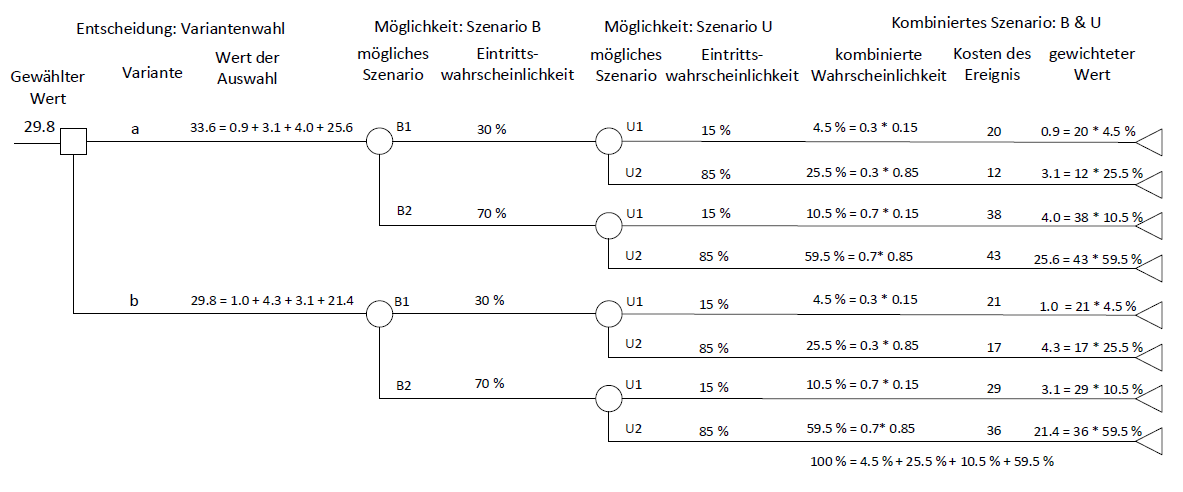
\includegraphics[width=\textwidth]{figures/f-02-02-EntscheidungsbaumBSP}
	\caption[Beispiel Entscheidungsbaum]{Beispiel eines Entscheidungsbaum}
	\label{img:EntscheidungBSP}
\end{figure}

Gesucht wird die Variante, welche die geringsten zuerwartenden Kosten und somit das kleinste Risiko generiert. Die Berechnung der Kosten erfolgt in diesem Beispiel von rechts nach Links, wobei der zeitliche Verlauf der Entscheidungssituation von links nach rechts dargestellt wird. 

\section{Sensitivitätsanalyse}
\label{sec:Sensitivität}

Ein wichtiger Bestandteil der Kosten-Nutzen Analyse ist, mithilfe einer Sensitivitätsanlyse zu untersuchen, wie stark ein Ergebniss von den getroffenen Annahmen abhängt und wie robust das Ergebniss auf eine Variation der Parameter reagiert. \\
Die Sensitivitätsanalyse kann sowohl mit den Nebenbedingungen als auch mit der Zielfunktion durchgeführt werden. In beiden Fällen wird untersuche was passiert bei einer Veränderung der ursprünglichen Annahmen und in welchem Rahmen können die Parameter verändert werden, ohne das sich das ursprüngliche Ergebniss verändert.  (\cite{Adey2019})

\pagebreak
 
\section{Real option methodology}
\label{sec:RealOption}

Die \textit{real option methodology} ist ein Vorgehen, um die optimale Variante einer Intervention, unter berücksichtigung von unsicheren zukünftigen Gegebenheiten, zu bestimmen. 
Sie ermöglicht es, Varianten einer Infrastruktur Intervention zu erarbeiten, die auf zukünftige veränderliche Rahmenbedingungen vorbereitet sind. So kann das einbeziehen von flexiblen Designs, im Prozess der Erschaffung einer Infrastrukturintervention, zusätzliche Vorteile generieren sowie zukünftige Risiken beseitigen. (\cite{Neufville2011})

Infrastrukturen sollten über einen längeren Zeitraum hinweg, ihre Serviceleistung auf einem angemessenen Niveau erbringen könnne. Dies setzt vorraus, dass sich die Infrastruktur an veränderliche Bedingungen anpassen und die Bedürfnisse der Interessensgruppen über einen längeren Zeitraum erfüllen, kann. 
Mit dieser Methodik kann, unter Berücksichtigung von unsicheren Variablen wie zum Beispiel der Veränderung der Anzahl Nutzer oder der Baukosten, ermittelt werden, welches Design den netto Nutzen des Investors am meisten vergrössert. (\cite{Esders2015})




% ===========================================================================
% EOF
%

%%% Local Variables:
%%% mode: latex
%%% TeX-master: "../main"
%%% End:


% Chapter 3
% ---------
%=============================================================================
% Thesis Template in LaTex
%
% File:  03-Vorgehen und Methodik -- Vorgehen
% Author(s): Cyrano Golliez <golliezc@student.ethz.ch>
%            
%
% Creation:  27 Jan 2014
% Time-stamp: <Tue 2013-08-13 20:14 juergen>
%
% Copyright (c) 2014 Infrastructure Management Group (IMG)
%               http://ibi.ethz.ch
%
% More information on LaTeX: http://www.latex-project.org/
%=============================================================================

\chapter{Vorgehen und Methodik}
\label{chap:Vorgehen}


Um eine Verbesserung der Verkehrssituation in Uster zu erreichen, müssen die unsicheren zukünftigen Gegebenheiten in der Generierung der Lösungsvarianten berücksichtigt werden. Eine optimale Variante zu erarbeiten, erfordert ein systematisches Vorgehen. 
Für das Bearbeiten der Problemstellung habe ich die Schritte und Überlegungen des Problemlösungsprozesses und der Real Option Methodology verwendet. Die nachfolgende Beschreibung, fast mein Vorgehen kurz zusammen.

\begin{IMleftrightskip}
Zur Bestimmung der Systemgrenzen wird eine Situationsanalyse durchgeführt. Mit dieser wird zum einen die Infrastruktur und zum anderen der Zeithorizont über den die Intervention untersucht wird, ermittelt. Zusätzlich werden die Faktoren, welche die zukünftigen Gegebenheiten in Uster am stärksten beeinflussen, definiert. Dies geschieht unter Berücksichtigung der momentanen Situation und der Annahmen, wie Uster in Zukunft funktionieren wird. Die Analyse schafft die Basis für die Formulierung der Ziele, welche in einem nächsten Schritt festgelegt werden.

Die Ziele legen fest, was mit der Intervention erreicht werden soll. Um zu bestimmen, was effektiv erreicht werden soll, müssen die betroffenen Parteien und ihre Bedürfnisse definiert werden. Für diese sogenannten Interessensgruppen werden alle relevanten Kosten ermittelt. Anhand dieser Kosten wird in einem nächsten Schritt die zu optimierende Zielfunktion definiert. Dann werden die relevanten Kosten definiert und die wichtigsten Einflussfaktoren, deren zukünftige Entwicklung ungewiss ist, bestimmt. 

Die nächste Phase umfasst das kreative Erschaffen von möglichen Lösungsvarianten, welche unter Berücksichtigung der jetzigen Situation erschaffen, werden. Um die optimale Variante bestimmen zu können, müssen diese analysiert, bewertet und verglichen werden. Dazu wird in einem ersten Schritt der Effekt der als unsicher definierten Einflussfaktoren, anhand von Szenarien modelliert. Um die Lösungsvorschläge unter dem Einfluss der verschiedenen Szenarien untersuchen zu können, müssen die Wahrscheinlichkeiten definiert werden, nach welcher ein Szenario eintreten wird. 

Der letzte Schritt zu Bestimmung der optimalen Variante beinhaltet die Bewertung der Lösungen. In dieser Phase wird mithilfe des Entscheidungsbaums das jeweilige Risiko der Varianten ermittelt. Um aufzuzeigen, wie die Veränderung der Parameter der Kostenstruktur das Ergebnis beeinflusst sowie um zu untersuchen, inwiefern sich das Ergebnis ändert, wenn die geschätzte Eintrittswahrscheinlichkeit der Szenarien variiert, wird eine Sensitivitätsanalyse durchgeführt. Eine Sensitivitätsanalyse erfolgt jeweils nur für einen Parameter, um deutlicher aufzeigen zu können, welchen Effekt diese Veränderung auf den Entscheidungsprozess hat. 
\end{IMleftrightskip}

Mit dem hier vorgestellten Vorgehen wird im Rahmen dieser Projektarbeit eine optimale Lösungsvariante zur Verbesserung der Verkehrssituation in Uster aufgezeigt. Nach dem Betrachten der zur Verfügung gestellten Literatur komme ich zum Schluss, dass eine solche Untersuchung bisher so noch nicht durchgeführt wurde. In den betrachteten Arbeiten wird jeweils nur ein Objekt hinsichtlich Flexibilität des Designs auf unsichere zukünftige Gegebenheiten untersucht. Das Bearbeiten eines gesamten Infrastruktursystems mit mehreren, sich gegenseitig beeinflussenden Komponenten wie zum Beispiel verschiedenen Verkehrsteilnehmern, Fussgängerzonen sowie Grün- und Parkanlagen, ist meines Erachtens, so noch nicht durchgeführt worden.

% ===========================================================================
% EOF
%

%%% Local Variables:
%%% mode: latex
%%% TeX-master: "../main"
%%% End:


% Chapter 4
% ---------
%=============================================================================
% Thesis Template in LaTex
%
% File:  2-Theory.tex -- Basic Theory
% Author(s): Jürgen Hackl <hackl@ibi.baug.ethz.ch>
%            Clemens Kielhauser <kielhauser@ibi.baug.ethz.ch>
%
% Creation:  27 Jan 2014
% Time-stamp: <Tue 2013-08-13 20:14 juergen>
%
% Copyright (c) 2014 Infrastructure Management Group (IMG)
%               http://ibi.ethz.ch
%
% More information on LaTeX: http://www.latex-project.org/
%=============================================================================

\chapter{Fallstudie}
\label{chap:Fallstudie}

Uster ist die dritt grösste Stadt im Kanton Zürich und liegt östlich des Greifensees. Die Stadt ist geprägt von der Entwicklung von einer dörflich geprägten Industriestadt zu einer Wohn- und Arbeitsstadt im ländlichen Umfeld. Aufgrund des angrenzenden Waldstück und der Nähe zum Greifensee, hat Uster einen hohen Freizeit und Erholungswert.
Die Entwicklung der Stadt aus mehreren Dörfern heraus, hat zur Folge, dass viele Einkaufsmöglichkeiten sowie Arbeitsplatzstandorte dezentral verteilt sind. Die historisch bedingte Verteilung der Büro- und Gewerbeflächen und die unterschiedlichen Standortqualitäten haben zu unterschiedlich ausgeprägten Stadtteilen geführt. Die Siedlungsgebiet in Uster wurden seit 1984 nicht mehr gross erweitert, weshalb ein weiteres Wachstum nur im Bestand möglich sein wird. Dies, und das unsichere zuküntige Bevölkerungswachstum, stellt für Uster eine grosse Herausforderung dar. (\cite{STEK}))

Das Berücksichtigen der Bedürfnisse der Bevölkerung von Uster, ist, um eine Optimierung der bestehenden Verkehrssystem zu erreichen, unabdingbar. Die Aufwertung des Stadtzentrum, die steigerung der Aufenthaltsqualität und die Verbesserung der Erreichbarkeit des Zentrum, haben für die Bevölkerung von Uster oberste Priorität. Dies soll, durch die Verkehrsberuhigung der zentrumsnahen Verkehrsnetze und durch die punktuelle Aufwertung der Strassenräume erfolgen. \\
Dass die Poststelle mit dem Auto, trotzt Zentrumsaufwertung, erreichbar bleibt, ist der Ustemer Bevölkerung ein weiteres wichtiges Anliegen. Zusätzlich wünscht die Bevölkerung, dass die nördlich des Bahnofs gelegenen Quartiere besser an das Zentrum angebunden und die Einkaufsmöglichkeiten in diesen Quartieren ausgebaut, werden. Dies setzt voraus, dass die Gleisquerung verbessert wird. Ausserdem hat die Bevölkerungsbefragung in Uster im Jahr 2015 ergeben, dass sich die Stadtbevölkerung einen Ausbau der Veloinfrastruktur wünscht, mit besonderem Augenmerk auf der Verbesserung der Situation an den Bahnübergängen. 

Um diese Bedürfnisse aussreichend befriedigen zu könne, wurde im STEK, die Ziele und strategischen Stossrichtungen der räumlichen Stadtentwicklung von Uster bis 2035 festgelegt. Der Stadtrat von Uster legt fest, dass auf Grundlage des STEK, die kommunalen Richt- und Nutzungspläne bis 2025 revidiert werden. Folglich nehme ich an, dass, um eine Prognosse für die Zukunft von Uster machen zu können, die Leitziele des STEK berücksichtigt werden müssen. Die Leitziele lauten gemäss (\cite{STEK}) wie folgt: 

\begin{description}
	\item[Stadtidentität]	\textit{Bewahrung und Weitereintwicklung der Vielseitigkeit} Die Stadt soll ihre polyzentrale Struktur behalten und die Vielseitigkeit der Innenstadt soll bewahrt werden. Uster soll in seiner Rolle als Regionalzentrum gestärkt werden, in dem das Wachstum auf das Zentrum und die gut erschlossenen Gebiete von Nänikon beschränkt wird.
	\item[Stadtentwicklung]	\textit{Wohnen und Arbeiten finden statt} Das Arbeitsplatzangebot soll sich im Gleichschritt mit dem Wohnungsmarkt entwickeln, um das Verhältniss von zwei Einwohnern auf einen Arbeitsplatz beizubehalten. Im Rahmen der Stadtentwicklung 2035, möchte die Stadt Uster, die zentrumsnahen Gebiete und die Bahnhofsumgebung in ein, mit Wohnungen durchmischtes Arbeitsplatgebiet umgestalten. 
	\item[Landschaft und Erholung] \textit{Grün- und Freiräume vor der Haustüre} Die Uster umgebenden Landschaften sollen erhalten und wo nötig aufgewertet werden und durch attraktive gestaltete Freiräume im Siedlungsgebiet, sowie durch gezieltes aufwerten der Erholungsräume, den Nutzungsdruck auf die Naturräume gemildert werden. 
	\item[Mobilität] \textit{Uster steigt um!} Um die Kapazitätsengpässe im bestehenden Verkehrsnetz zu mildern, erwägt Uster einen Umstieg vom motorisierten Individualverkehr kurz. MIV auf den öffentlichen Verkehr, kurz. ÖV, und auf den Langsamverkehr, sprich Velo- und Fussgängerverkehr. Die Stadt Uster setzt sich zum Ziel, eine Reduktion des MIV Anteil am Modalsplit des innerstädtischen Verkehr zuerreichen und den Langsam- sprich Veloverkehr nachhaltig zu fördern. Dies geschieht durch die Verbesserung der Routen und Fahrbedingungen des Veloverkehrs. Insbesondere im Zentrum, wird die Verkehrsführung angepasst, um einerseits die Erreichbarkeit mit dem Velo zu verbessern und andererseits die Aufenthaltsqualität durch die lokale Verkehrsberuhigungen zu erhöhen.
\end{description}

Im Rahmen des Leitbild \textit{Stadtraum Uster 2035} werden im STEK sogenannte Schlüsselprojekte definiert. Als Schlüssprojekte bezeichnet, werden Interventionen, die durch ihre Ausführung, in ihrer Umgebung eine weitere Entwicklung auslösen sollen. Die wichtigsten Schlüsselprojekte sind; das Bahnhofsgebiet, das verkehrsberuhigte Zentrum, das Zeughausareal, die Erhohlungsachse Aabach, die urbane Strassenraumgestaltung im Zentrumsgebiet und die Fuss- und Velounterführung Brunnen-/Bahnhofstrasse, sowie die beiden kantonalen Projekte zur Stadterschliessung; Usterwest und Umfahrung Moosackerstrasse. Das Ausmass, der aufgrund der Ausführung dieser Projekte entstehenden Auswirkungen auf die Verkehrsleistung in Uster, kann nicht mit absoluter Sicherheit vorher gesagt werden. (\cite{STEK}) \\

Die Stadtentwicklung sieht vor, dass das Zentrum von Uster attraktiv umgestalt wird. Diese Zentrumsentwicklung soll, durch bauliche Verdichtung die Nachfrage vor Ort steigern. Durch die Aufwertung des Strassenraums und durch Massnahmen zur Verkehrsberuhigung, soll das Zentrum für Velofahrer besser erreichbar werden, wobei die Erreichbarkeit mit dem Auto gewahrt bleiben soll. Die Umgestaltung der Strassenräume der Innenstadt, zu urbanen Begegnungszonen, erfordert eine Anpassung der Verkehrsregime. \\
Aufgrund dessen, dass die Versorgungslage im Stadtzentrum die Standortqualität von Uster als Wohn- und Arbeitsstadt beeinflusst und dass die Bevölkerungsbefragung ergeben hat, dass die steigerung der Attraktivität des Zentrums für die Bevölkerung von hohem Interesse ist, hat die Zentrumsentwicklung, höchste Priorität. \\
Gemäss der STEK haben die bahnhofsnahen Grundstücke die grössten Wachstumpotentiale. Das heisst, dass die Umnutzung dieser Grundstücke infolge der Aufwertung des Stadtzentrums, mit grösster Wahrscheinlichkeit zu einer Erhöhung der Verkehrsbelastung am Bahnhof und den zentrumsnahen Vekehrsnetzen, führen wird. Insbesondere auf dem Velonetz, ist infolge dessen, mit einer in der Zukunft erhöhten Belastung zurechnen. 
(\cite{STEK})

\paragraph{Verkehr} ist in Uster ein politisch äusserst umstrittenes Thema. Das Zentrum ist stark geprägt durch den MIV und ein nahezu flächendeckendes Tempo 30 Regime. Der Quell- und Zielverkehr in Zentrum und der hauptsächlich in Nord-Süd Richtung erfolgende Durchgangsverkehr, haben ein hohes Verkehrsaufkommen im Zentrum zur Folge. Die Aufenthaltsqualität auf den wichtigsten Strassen im Zentrum, wie zum Beispiel der Bankstrasse und der Bahnhofstrasse, ist durch die hohe Verkehrsbelastung, reduziert. Insbesondere die Bankstrasse ist zu Spitzenbelastungszeiten ein Nadelöhr im ÖV-Netz, da das grosse Verkehrsaufkommen, das An- und Abfahren der Busse erschwert. \\
Ausserdem, um möglichst kurze Wartzeiten zu ermöglichen, erreichen alle Buslinien den Bahnhof zur selben Zeit. Dies hat eine hohe Belastung der bahnhofsnahen Verkehrsinfrastruktur zur Folge. \\
Durch die Kombination aus S-Bahn und bis zu sechs Stadtbuslinien, ist Uster durch den öffentlichen Verkehr in grossen Teilen erschlossen. Jedoch hat der, durch den grosse Anteil an MIV am innerstädtischen Verkehr entstehenden Stau, zur Folge, dass die Fahrplanstabilität des ÖV beeinträchtigt wird. (\cite{STEK})

Uster erwartet aufgrund des Bevölkerungs- und Arbeitsplatzwachstum eine Zunahme des Verkehrsaufkommen. Um eine ausreichende Mobiliät gewährleisten zu können und die Umweltbelastung zu reduzieren, hat Uster, im Rahmen des Gesamtverkehrskonzept des Kanton Zürichs, zwei Ziele formuliert. Zum einen soll die Erreichbarkeit der urbanen Räume verbessert und zum anderen,durch gezielte Eingriffe, eine Erhöhung des Langsamverkehrsanteil am Gesamtverkehrsaufkommen erwirkt werden. Das Langsamverkehrsnetz, sprich Velo- und Fusswegenetz, ist gemäss dem STEK, vorallem auf den kurzen und zentrumsnahen Hauptrouten zu stärken. Gemäss kantonalem Richtplan soll der Anteil des Langsamverkehrs am Gesamtverkehrsaufkommen, von 20\% (2011) auf 22\% (2030) erhöht werden. Dies bedingt, dass der Modalsplit des Innerstädtischenverkehr zugunsten des Langsamverkehrs verändert wird. Jedoch soll die Kapazitäten des MIV weder erhöht, noch merklich reduziert werden. 

Gemäss dem STEK beträgt der MIV-Anteil am innerstädtischen Ziel-, Quell- und Binnenverkehr 57\%. Demnach sind die Verkehrsprobleme von Uster mehrheitlich selbst verursacht. Weiter hat das sternförmig angelegte Strassennetz, hat zur Folge, dass der Nord-Süd Durchrgangsverkehr mehrheitlich, durch das Stadtzentrum geführt wird. Die wichtigsten Knotenpunkte, wie zum Beispiel der Nüsslikreisel, der Nashornkreisel sowie die Seefeldstrasse, geraten in den Spitzenbelastungszeiten an ihre Kapazitätsgrenzen.

\begin{figure}[h!]
	\centering
	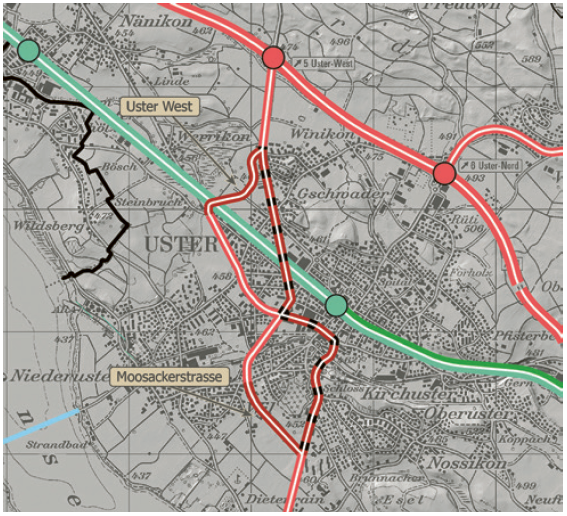
\includegraphics[width=\textwidth]{figures/04-04-UsterWest-Moosackerstr}
	\caption[Strassenprojekte im Kantonalen Richtplan]{Moosackerstrasse und Usterwest gemäss (\cite{STEK})}
	\label{img:Strassenprojekte}
\end{figure}

Die Abbildung \ref{img:Strassenprojekte} zeigt die geplanten kantonalen Strassenprojekte Usterwest und Moosackerstrasse. Durch diese Strassenprojekte, sollen einerseits die Stadterschliessung verbessert und andererseits das Zentrum vom Durchgangsverkehr entlastet werden. Insbesondere die Verkehrsbelastung des Nüsslikreis, soll durch den Bau der Moosackerstrasse reduziert werden. Gemäss dem STEK ist die Realisierung der Uster Westumfahrung in näherer Zukunft nicht absehbar. Mit dem Bau der Moosackerstrasse hingegen, kann in näherer Zukunft gerechnet werden, was zu einer Reduktion des Durchgangsverkehr im Zentrum und einer Entlastung des Nüsslikreisel führen wird. Laut dem STEK wird die Situation an den bestehenden Bahnübergängen, durch den Bau der Moosackerstrasse nicht verbessert. Um die Situation an den Bahnübergängen nachhaltig zu verbessern, muss ein anderer Lösungsansatz gefunden werden. 

\begin{figure}[h!]
	\centering
	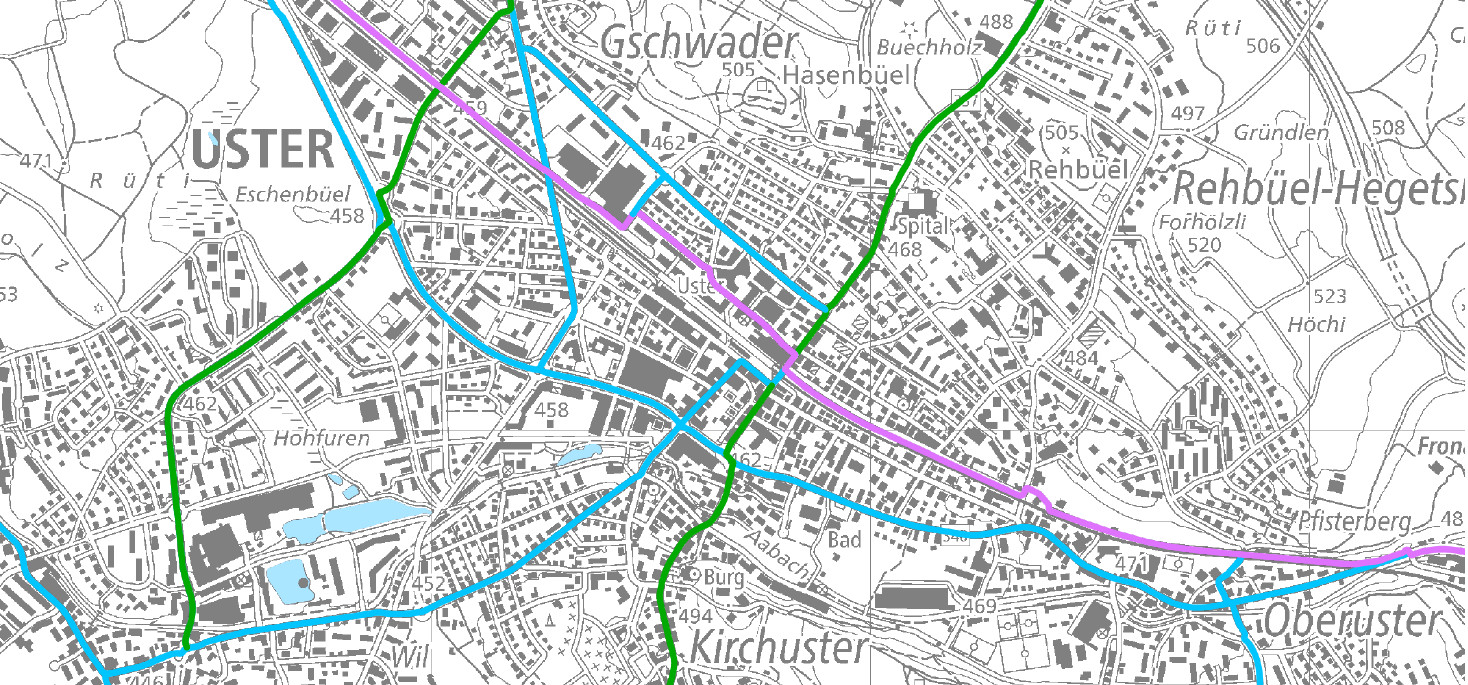
\includegraphics[width=\textwidth]{figures/04-01-Veloweg-Alltag}
	\caption[Velonetz Alltag]{Velonetz Alltag (\cite{GIS})}
	\label{img:Velonetz}
\end{figure}
 
Die Abbildung \ref{img:Velonetz} zeigt das Velonetz der Innenstadt von Uster. In grün sind die Hauptverbindungen, in blau die Nebenverbindungen und in violett die Veloschnellroute dargestellt. Wie in der Abbildung ersichtlich, ist der Bahnübergang Brunnenstrasse der zentrale Knotenpunkt des Velonetz. Die Gleisquerung ist für den Langsamverkehr, aufgrund des dichten S-Bahn Fahrplans, nur mit langen Wartezeiten möglich. 

Gemäss der Leitziele, die sich Uster im Rahmen der Stadtenticklung 2035 gegeben hat, soll Uster zur Velostadt ausgebaut werden. Die von der SP eingereichte Velointiative wiederspiegelt das Bedürfnis der Bevölkerung nach einer Förderung des Langsamverkehrs. Insbesondere die, im kantonalen Städtevergleich, als unterdurchschnittlich erachtete Dichte des Velonetz, stellt für die Bevölkerung ein Mangel dar. Ausserdem ist die Verkehrssicherheit, aufgrund der stark am MIV ausgerichten Strassenräume, auf dem bestehenden Velonetz mangelhaft. \\
So fordert die Bevölkerung von Uster eine zukunftsorientierte Gestaltung des Velonetz, insbesonder unter Berücksichtigung der neuen Velotypen, wie Lastenräder und schnellen E-Bikes, sowie der Verbesserung der Möglichkeit zu Querung der Gleisanlagen. 

Die Erhöhung der Sicherheit auf dem bestehenden Velonetz, die Verbesserung der Gleisquerung und die damit einhergehenden Erhöhung der Erreichbarkeit des Zentrums durch den Langsamverkehr, erachte ich, als die zentralen Punkte, um eine Verbesserung der Verkehrssituation in Uster zu erreichen. Die geplante Erhöhung des Langsamverkehrsanteil am innerstädtischen Modalsplit und der Ausbau der Veloparkieranlagen in bahnhofsnähe, werden zukünftig zu mehr Veloverkehr führen. 

Nach der Analyse des STEK, bin ich zum Schluss gekommen, dass die Zerschneidung der Stadt, durch die Gleisanlage, eines der grössten Probelem von Uster ist. Aufgrund dessen und unter Berücksichtigung der Leitziele des STEK den Langsamverkehr zu fördern, habe ich mich dazu entschieden, den Bahnübergang Brunnenstrasse, für den Veloverkehr zu optimieren, um einen nachhaltige Verbesserung der Verkehrssituation zu erreichen. 

\begin{figure}[h!]
	\centering
	\includegraphics[width=0.6\textwidth]{figures/04-01-Bahnübergang-FOTO}
	\caption[Bahnübergang Brunnenstrasse]{Bahnübergang Brunnenstrasse und Velonetz Alltag (\cite{GIS})}
	\label{img:Brunnenstrasse}
\end{figure}

Die Abbildung \ref{img:Brunnenstrasse} zeigt den Bahnübergang Brunnenstrasse. Diese Infrastruktur verbindet die südlich des Bahnhofs gelegenen Stadteile mit dem Spital und der Sportanlage Buchholz, sowie die nördlich des Bahnhofs gelegenen Quartiere mit dem Stadtzentrum und dem Greifensee. 

Die von mir erarbeitete Intervention, soll die Situation am Bahnübergang nachhaltig verbessern. Deshalb untersuche ich, im Rahmen dieser Arbeit, den Effekt dieser Varianten auf die Verkehrssituation, über einen Zeitraum von vierzig Jahren. Um das beste Investment für die Stadt Uster, ermitteln zu können, definiere ich im nachfolgenden Abschnitt, die Ziele die mit der Intervention erreicht werden sollen.

\pagebreak

\section{Formulierung der Ziele und Rahmenbedingungen}
\label{sec:Zielformulierung}

In Anbetracht der dezentralen Struktur von Uster und der geplanten Umgestaltung der Innenstadt zur Begegnungszoneist, ist eine Verbesserung der Erreichbarkeit des Zentrums unabdingbar. Eine Verbesserung der Erreichbarkeit setzt vorraus, dass die Reisezeit verkürzt und die Verkehrssicherheit erhöht wird. Das bedeuted, dass die Möglichkeit zur Gleisquerung ausgebaut und mit einer besseren Signalisation ausgestatt wird. Weiter soll die Zerschneidung der Stadt, durch die Gleisanlage entschärft und so einen wichtigen Beitrag zur Stadtentwikcklung geleistet werden. Die von mir geplante Infrastruktur Intervention, soll die Verkehrssituation am Bahnhof nachhaltig verbessern, sowie die Attraktivität und die Standortqualitäten von Uster stärken.
Das Ziel der Intervention soll demnach sein, der gesteigerten Nachfrage nach Mobilität Rechnung zu tragen, sowie den Langsamverkehrsanteil am Modalsplit des Innenstadtverkehrs zu erhöhen, unter Berücksichtigung der unsicheren zukünftigen Gegebenheiten.

Um ermitteln zu können, welche Variante einer Intervention die beste ist, muss in einem ersten Schritt definiert werden, was als \textit{am besten} erachtet wird. Dafür müssen die Bedürfnisse der beteiligten Personen berücksichtigt werden. \\
Um zu bestimmen, was für diese Personen \textit{am besten} ist, müssen ihre, durch die Infrastruktur entstehenden Kosten und Nutzen berücksichtigt werden.
 
Das Ziel meiner Optimierung ist, durch die minimierung der Kosten, den Gesamtnutzen aller Interessensgruppen zu steigern. Aufgrund dessen, dass in der nachfolgenden Berechnung, nur die Kosten der beteiligten Personen berücksichtigt wird, ist die Minimierung der Kosten, mit der Maximierung des Nutzens gleichzusetzen. \\
So sollen einerseits, durch die Reduktion der Reisezeit die Kosten der Nutzer reduziert werden und andererseits, durch die Erhöhung der Verkehrssicherheit, die Kosten der Allgemeinheit reduziert werden. 



	\subsection{Interessensgruppen}
	%=============================================================================
% Thesis Template in LaTex
%
% File:  Interessensgruppen -- Fallstudie
% Author(s): Jürgen Hackl <hackl@ibi.baug.ethz.ch>
%            Clemens Kielhauser <kielhauser@ibi.baug.ethz.ch>
%
% Creation:  27 Jan 2014
% Time-stamp: <Tue 2013-08-13 20:14 juergen>
%
% Copyright (c) 2014 Infrastructure Management Group (IMG)
%               http://ibi.ethz.ch
%
% More information on LaTeX: http://www.latex-project.org/
%=============================================================================

% Unterkapitel Interessengruppen
% ---------
\label{subsec:Gruppen}

\begin{description}
\item[Besitzer]\hfill \\
Die Interessensgruppe der Eigentümer setzt sich aus verschiedene Parteien zusammen. Die wichtigsten involvierten Parteien sind die Stadt Uster und der Kanton Zürich sowie die Eigentümerin der Sportanlage Buchholz. Sie werden durch die Baudirektion der Stadt Uster vertreten.
Für die Besitzerin der Infrastruktur wird in dem betrachteten Zeitraum nur die Initialisierungskosten sowie die laufenden Betriebskosten von Bedeutung sein. Um ein vollständiges Bild der Interessen der Besitzer zu erhalten, müssten weiter Kosten in Betracht gezogen werden. 
Für unsere Untersuchungen, welche die Infrastruktur in den nächsten 40 Jahren betrachtet, spielen die Unterhaltskosten die bedeutendste Rolle. Einerseits übersteigt die W'keit, dass diese Kosten bezahlt werden müssen, die W'keit dass andere Kostentypen eintreten und andererseits ist der absolute Betrag der Unterhaltskosten über einen Zeitraum von $T$ Jahren deutlich grössers als der anderer Kostentypen. Aufgrund dieser Überlegungen brachten wir für die Besitzer nur die Unterhaltskosten. 
\item[Nutzer]\hfill \\ 
Für die nachfolgende Optimierung ist es von zentraler Bedeutung die massgebenden Kostenstrukturen zu definieren. In anbetracht der Verkehssituation, sind die  folgenden Kostentypen diejenigen die für den Nutzer massgebenden sind. 
Der Nutzer der Infrastruktur ist der Langsamverkehr der gemäss STEK sämtliche Verkehrsmitteln einschliesst die aus eigener Kraft angetrieben werden. Es muss geprüft werden ob auch Sonderbewilligungen zur Nutzung der Infrastruktur für E-Bikes und Hybridräder erteilt werden kann. Dies sollte nur geschehen fals die geplannte Kapazität der Infrastruktur das befahren mit deutlich unterschiedlichen Geschwindigekeiten erlaubt.
Die Infrastruktur ist für jegliche Art von nichtmotorisiertem Verkehr ausgelegt. Dieser beinhaltet Fahrräder, Inlineskater, Skateboarder und auch Rollstuhlfahrer.Wichtig für die planung der Intervention ist die Unterteilung der Verkehrsteilnehmer anhand ihrer durchschnittlichen Geschwindigkeit.
\item[Öffentliche Hand]\hfill \\
Die in Tabelle \ref{tab:t-04-01-Interessensgruppen} aufgeführten Kosten sind die massgebenden Einwirkungen auf die Allgemeinheit. Die Öffentliche Hand setzt sich aus direkt und indirekt betroffener Personen zusammen. 
Die Anwohner sowie in einem entfernteren Sinne auch die Nutzer selbst, zählen zur direkt betroffenen Öffentlichkeit. Sie nutzen die Infrastruktur nicht direkt, befinden sich aber in ihrer unmittelbaren Nähe. Diese sind die Hauptträger der Kosten die durch Lärm- und Schadstoffbelastung enstehen. Eine Reduktion des MIV Anteil und die damit einhergehende verkehrsberuhigung sind die besten Mittel zur Reduktion dieser Kosten.   \\
Die Unfallkosten gehen zulasten der Allgemeinheit in Form der Belastung des Gesundheitssystems. Die Allgemeinheit nutzt in diesem Sinne die Infrastruktur nicht und ist auch nicht in ihrer Nähe zuhause oder bei der Arbeit sondern wird durch die Benützung der Infrastruktur von ihr indirekt betroffen.
\end{description}




% ===========================================================================
% EOF
%

%%% Local Variables:
%%% mode: latex
%%% TeX-master: "../main"
%%% End:


	\subsection{Zielfunktion}
	%=============================================================================
% Thesis Template in LaTex
%
% File:  Zielfunktion -- Fallstudie
% Author(s): Jürgen Hackl <hackl@ibi.baug.ethz.ch>
%            Clemens Kielhauser <kielhauser@ibi.baug.ethz.ch>
%
% Creation:  27 Jan 2014
% Time-stamp: <Tue 2013-08-13 20:14 juergen>
%
% Copyright (c) 2014 Infrastructure Management Group (IMG)
%               http://ibi.ethz.ch
%
% More information on LaTeX: http://www.latex-project.org/
%=============================================================================

% Unterkapitel Zielfunktion
% ---------
\label{subsec:Funktion}


Das Ziel meiner Optimierung ist es den Gesamtnutzen zu steigern mit speziellem Augenmerk auf der Vermehrung des Nutzens der Fahrradfahrer.

Die geplanten Infrastruktur Interventionen sollen die Kapazität und somit das Angebot auf der Route Bahnhof - Sportanlage erhöhen. 

Mithilfe der Optimierung und der anschliessenden Analyse soll diejenige Intervention bestimmt werden, die den totalen Nutzen über den betrachteten Zeitraum am meisten steigert. 


Die Gleichung \ref{equation:1} stellt das Optimierungsproblem als mathematische Funktion dar.
Die totalen Kosten $TK$ einer Interventionsstrategie sind definiert als die netto Kosten aller Steakholder über einen untersuchten Zeitraum $[0,T]$ 

Da in userem Fall die Erlöse, während einer Zeitperiode $[0,T]$ generiert werden können, nicht in Betracht gezogen werden, ist die minimierung der Gesamtkosten äquivalent zur maximierung des netto Nutzens aller beteiligter Interessensverände. 
Die Zeit $0$ kennzeichnet den Startpunkt der Untersuchung wobei die Zeit $T$ das Ende der Untersuchungsperiode ist. 

\begin{equation}
Min. \thinspace TK_{i} = Min. \thinspace [K_{U}^i + K_{TT}^i + K_{B}^i + K_{E}^i + K_{A}^i]
\label{equation:1}
\end{equation} 

{\setstretch{0.75}
wobei:
\begin{conditions}
\renewcommand{\arraystretch}{0.7}
 TK_{i}   	    &  Totale Kosten der Variante $i$ für den betrachteten Zeitraum von $T$ Jahren \\
 K_{U}^i		&  Totale Unterhalts- und Baukosten der Variante $i$ \\
 K_{TT}^i       &  Totale Reisezeitkosten der Variante $i$    \\
 K_{B}^i        &  Totale Betriebskosten der Variante $i$ \\
 K_{E}^i	    &  Totale Umweltbelastungskosten der Variante $i$  \\
 K_{A}^i        &  Totale Unfallkosten der Variante $i$ 
\end{conditions}
}

Tabelle \ref{tab:t-04-01-Interessensgruppen} listet die Interessensgruppen sowie die Kostenstrukturen auf. Die Kostenstrukturen in Form der Kostentypen und der modelierten Einheitskosten werden in den folgenden Kapitel erläutert .

%=============================================================================
% Thesis Template in LaTex
%
% File:  t-05-01-IsingModel.tex -- Table for the Ising
% Author(s): Juergen Hackl <hackl@ibi.baug.ethz.ch>
%            Clemens Kielhauser <kielhauser@ibi.baug.ethz.ch>
%
% Creation:  27 Jan 2014
% Time-stamp: <Tue 2013-08-13 20:14 juergen>
%
% Copyright (c) 2014 Infrastructure Management Group (IMG)
%               http://ibi.ethz.ch
%
% More information on LaTeX: http://www.latex-project.org/
%=============================================================================

\begin{table}[ht!]
\flushleft
\renewcommand{\arraystretch}{1.4}
%\small\renewcommand{\arraystretch}{1.2} 
%
%
\begin{tabular}{@{}p{3.3cm} p{4cm} p{1.2cm} r l @{}} \\   
\toprule
\textbf{Interessensgruppe} & \textbf{Kostentyp} & \textbf{Symbol} & \multicolumn{2}{c}{\textbf{Einheitskosten}} 			\\
\midrule
Besitzer                   & Unterhaltkosten (\textit{U})                    & $K_{U}(t)$    & 5 - 30 		&	$\frac{CHF}{m^2 \ Jahr}$              \\
Nutzer		               & Reisezeitkosten (\textit{TT})                   & $K_{TT}(t)$   & 35 - 56 		&	$\frac{CHF}{Stunde \ DTV_{k}}$         \\
                           & Betriebskosten (\textit{B})            		 & $K_{B}(t)$    & 0.15 - 0.7 	&	$\frac{CHF}{km \ DTV_{k}}$              \\
Öffentliche Hand           & Kosten durch Belastung \newline der Umwelt \newline (Environment) (\textit{E})   & $K_{E}(t)$    & 0.05  & $\frac{CHF}{Fahrzeugkilometer}$      \\
                           & Unfallkosten (\textit{A})                       & $K_{A}(t)$    & 15'000 - 3.7mio & $\frac{CHF}{Unfall_{n}}$    \\
\bottomrule

\end{tabular}
\caption{Tabelle der Interessensgruppen und Kostenstrukturen}
\label{tab:t-04-01-Interessensgruppen}
\end{table}


%=============================================================================
% EOF
%

%%% Local Variables:
%%% mode: latex
%%% TeX-master: "../guidelines"
%%% End:



\newpage

% ===========================================================================
% EOF
%

%%% Local Variables:
%%% mode: latex
%%% TeX-master: "../main"
%%% End:

	
\pagebreak

\section{Kostenstruktur}
\label{sec:Kostenstruktur}

Um das Risiko, welches von einer Infrastruktur Intervention ausgeht, berechnen zu können, muss die verwendete Kostenstruktur definiert werden. 
Im allgemeinen erfolgt die approximation der Kosten durch die Bestimmung der relevanten Faktoren wie zum Beispiel der Länge und der Breite der Infrastruktur, des täglichen Verkehrsaufkommens, der benötigten Reisezeiten sowie weiterer Faktoren. Die ermittlung der Kosten erfolgt im Anschluss durch die Multiplikation dieser Faktoren mit den dazugehörigen Einheitskosten. (\cite{Adey2012}) 

%=============================================================================
% Thesis Template in LaTex
%
% File:  Kostenstruktur -- Fallstudie
% Author(s): Jürgen Hackl <hackl@ibi.baug.ethz.ch>
%            Clemens Kielhauser <kielhauser@ibi.baug.ethz.ch>
%
% Creation:  27 Jan 2014
% Time-stamp: <Tue 2013-08-13 20:14 juergen>
%
% Copyright (c) 2014 Infrastructure Management Group (IMG)
%               http://ibi.ethz.ch
%
% More information on LaTeX: http://www.latex-project.org/
%=============================================================================

% Unterkapitel Kostenstruktur
% ---------
\label{subsec:Kosten}

\newpage

In diesem Kapitel werden die Kosten, die für die verschienden Interessensverbände enstehen, erläutert und ihre Berechnung dargestellt.  \\
Um das Risiko, welches von einer Infrastruktur Intervention ausgeht, berechnen zu können, muss die verwendete Kostenstruktur definiert werden. 
Im allgemeinen erfolgt die approximation der Kosten durch die Bestimmung der relevanten Faktoren wie zum Beispiel der Länge und der Breite der Infrastruktur, des täglichen Verkehrsaufkommens, der benötigten Reisezeit sowie weiterer Faktoren. Die ermittlung der Kosten erfolgt im Anschluss durch die Multiplikation dieser Faktoren mit den dazugehörigen Einheitskosten.\footcite{Adey2012} \\
Die von 


\subsubsection{Unterhaltskosten}
\label{subsub:Unterhalt}

Die Berechnung der Unterhaltskosten $K_{U}$ der Infrastruktur werden in Formel \ref{eq.2} dargestellt. Sie setzen sich zusammen aus den einmaligen Investitionskosten für den Bau der Infrastruktur $K_{Bau}$ und den jährlich anfallenden Wartungskosten $K_{Wartung,t}$ gemäss Formel \ref{eq.3}. Die Baukosten und die Einheitskosten der Wartung werden nachfolgend erläutert.


\begin{align}
K_{U} &= K_{Bau} + \sum_{t=0}^T \  K_{Wartung,t}  \label{eq.2} \\
K_{Wartung,t} &= \sum_{t=1}^2 \ EK_{Wartung,k} \cdot s_{k} \cdot b_{k}  \label{eq.3} 
\end{align}

\begin{align*}
	  k &=
      \begin{cases}
        \begin{aligned}
          & 1 \\
          & 2
        \end{aligned} &
        \begin{aligned}
         & \text{für}\ \thinspace \\
         & \text{für}\ \thinspace
        \end{aligned}
        \begin{aligned}
          & Strasse \\
          & Unterfu"hrung
        \end{aligned}
      \end{cases} \\
\end{align*}

{\setstretch{0.6}
wobei:
\begin{conditions}
 K_{U}      	     			&  Totale Unterhaltskosten für $T$ Jahre  \\
 K_{Bau}           			    &  Baukosten der Variante     \\
 K_{Wartung,t}                  &  Wartungskosten pro Jahr     \\
 EK_{Wartung,k}      	     	&  Einheitskosten pro $m^2$   \\
 s_k	    	     			&  Länge der Infrastruktur in $m$ \\
 b_k	    	     			&  Breite der Infrastruktur in $m$   \\
 k								&  Art der Infrastruktur  
\end{conditions}
}

Die entstehenden Investitionskosten für den Bau der verschiedenen Instrastrukturen, habe ich nach \cite{Baukosten2010} folgendermassen angesetzt. Die Erstellung zweier neuer Radstreifen à $1.5 \, m$ Breite kostet $850 \, CHF$ pro Laufmeter. Die Investitionskosten pro Quadratmeter für den Bau einer Velounterführung unter dem Lastfall Eisenbahn, betragen $3750 \, CHF$. Der Bau der Zufahrtsrampen zu den Velounterführungen kostet pro Rampe $130'000 \, CHF$. 
Die Wartungskosten der verschiedenen Infrastruktur Typen habe ich nach einem Gespräch mit Herr Dr. Martani wie folgt angesetzt. Für die Instandhaltung der Strasse, inklusive der Fahrradstreifen und der Fussgängerwege nehme ich an, dass jährlich $5 \thinspace \frac{CHF}{m^2}$ anfallen. Die wartungsintesivere Infrastruktur der Unterführung wird jährlich mit $30 \thinspace \frac{CHF}{m^2}$ instand gehalten.  

\newpage

\subsubsection{Reisezeitkosten}
\label{subsub:Reisezeit}


Die beim benutzen der Infrastruktur enstehenden Reisezeitkosten ($TT$) (engl. Travel time cost), spiegeln die wirtschaftlichen Auswirkungen des Zeitverlustes auf den Verkehrsteilnehmer wieder und sind somit die Kosten der Reise in Form von Zeitverlust. In Anbetracht der Tatsache, dass in dieser verlorenen Zeit gearbeitet, sowie Freizeit verbracht hätte werden können, kann dieser Zeitverlust monetär beziffert werden. Dies erfolgt mit den nachfolgen beschriebenen Einheitskosten des Zeitverlustes.  
Die Berechnung der totalen Reisezeitkosten $K_{TT}$ für $T$ Jahre erfolgt gemäss Formel \ref{eq.4} und ist eine Vereinfachung der Berechnung der \textit{Travel time cost} \cite[vlg.][643]{Adey2012}.
  

\begin{align}
K_{TT} &= \sum_{t=0}^T \Biggl[ \sum_{j=1}^2 \ DTV_{j} \cdot t_{j} \cdot EK_{TT,j} \Biggr] \label{eq.4} \\
t &= \frac{s_{k}}{v_{j}} \Biggl( 1 + 0.15 \Bigl(\frac{DTV_{j}}{C_{j}} \Bigr)^4 \Biggr) \label{eg.5} 
\end{align}

\begin{align*}
	 j &=
      \begin{cases}
        \begin{aligned}
          & 1 \\
          & 2
        \end{aligned} &
        \begin{aligned}
         & \text{für}\ \thinspace \\
         & \text{für}\ \thinspace
        \end{aligned}
        \begin{aligned}
          & für MIV \\
          & für Velo
        \end{aligned}
      \end{cases} \\
\end{align*}

{\setstretch{0.75}
wobei:
\begin{conditions}
 K_{TT}		 	 &  Totale Reisezeitkosten für $T$ Jahre  \\
 DTV_{j}    	 &  Tägliches Verkehrsaufkommen nach Fahrzeugtyp \\
 t_{j} 			 &  Zeitverlust nach Fahrzeugtyp \\
 EK_{TT,j} 		 &  Einheitskosten der verlorenen Zeit  \\
 v_{j}			 &  Gefahrene Geschwindigkeit nach Fahrzeugtyp \\
 C_{j}			 &  Kapazität der Infrastruktur nach Fahrzeugtyp  \\
 j				 &  Art des Fahrzeugs   
\end{conditions}
}

Der Zeitverlust ist abhängig vom Zustand der Infrastruktur, genauer von der Beschaffenheit des Oberflächenbelags der Fahrbahn. sowie der momentanen Auslastung. Diese Beziehungen ist schwierig zu modelieren. Jedoch kann zwischen dem Zeitverlust auf der Infrastruktur, dem Auslastungsgrad, in Abhängigkeit von der gebauten Variante und der gefahrenen Geschwindigkeit eine Beziehung modeliert werden. Diese Approximation ermöglicht es mir, die verlorene Zeit, gemäss \ref{eg.5} zu berechnen.  
Die Zeit die man benötigt eine bestimmte Strecke zurück zu legen ist abhängig von der gefahrenen Geschwindigkeit welche wiederum abhängig ist vom Zustand der Strasse sowie der Kapazität der Infrastruktur. Wird die Kapazität durch eine zu hohe Nachfrage überschritten, kann dies zu einer Überlastung des Systems führen und somit zu Verstopfungen und daraus resultierenden Verspätungen.  

Die Einheitskosten der verlorenen Zeit $EK_{TT,j}$ werden anhand des schweizerischen Medianlohn von 2018 berechnet. Der Medianlohn betrug im Jahr 2018 $6538 \, CHF$ pro Monat bei einer durchschnittlichen Arbeitszeit von 42,5 Stunden pro Woche (Quelle: BFS). Daraus ergibt sich einen durchschnittlichen Bruttostundenlohn von $38,5 \, CHF/h$ pro Person, was im Falle dieser Berechnung den Einheitskosten der verlorenen Reisezeit eines Velofahrers entspricht. Unter der Annahme eines durchschnittlichen Auslastungsgrad von 1.6 Personen pro Fahrzeuge \cite{Mikrozensus2015}, betragen die Einheitskosten der verlorenen Reisezeit pro Fahrzeug $61,6 \, CHF/h$.



\subsubsection{Betriebskosten}
\label{subsub:Betrieb}


Die Betriebskosten $K_{B}$ die für die Nutzer der Infrastruktur, für den betrachteten Zeitraum von $T$ Jahren, anfallen, werden gemäss Formel \ref{eq.6} berechnet. So werden die Betriebskosten aus der Multiplikation der Anzahl Nutzer und der zurückgelegten Distanz mit den Einheitskosten pro Fahrzeugkilometer ermittelt.
Diese sogenannten Fahrzeugsbetriebkosten sind im Rahmen dieser Optimierung, als die jährlich pro Nutzer anfallenden Wartungskosten definiert und sind somit die Kosten, die für die Instandsetzung und den Betrieb eines Fahrzeugs, bei benützung der Infrastruktur, entstehen können. Diese setzen sich zusammen aus den Kosten der Arbeitssstunden für die Instandsetzung sowie der Kosten für die Ersatz- und Verschleissteile.
 
Diese Kosten sind abhängig von der Qualität des Fahrbahnbelags, von der Ausführung der Infrastruktur und von der Kapazität der Infrastruktur. Weiter ist ein entscheidender Faktor in der Bestimmung der Fahrzeugbetriebskosten die Strassengeometry. Diese beinhaltet die Anzahl und Form der Kurven, die Steigungen sowie die Breite der Strasse und die daraus resultierende Möglichkeit des sicheren Überholens. Die Anzahl an Kreuzungsstellen und die davon abhänginge Anzahl an Brems- und Beschleunigungsmanöver haben einen direkten Einfluss auf den Verschleiss der Mechanik des Fahrzeugs. So werden im Falle des Fahrrads die Kette und die Bremsbeläge durch vermehrtes Bremsen und Anfahren verstärkt abgenutzt und im Falle des Autos erhöhen sich die Betriebskosten bei vermehrtem \textit{Stop-and-Go} Verkehr.

\begin{equation}
K_{B} =  \sum_{t=0}^T \Biggl[ \sum_{j=1}^2 \ EK_{B,j} \cdot s_{k} \cdot DTV_{j} \Biggr]  \label{eq.6} \\
\end{equation}

{\setstretch{0.75}
wobei:
\begin{conditions}
 K_{B}			   &  Totale Fahrzeugbetriebskosten \\
 EK_{B,j}	       &  Einheitskosten pro $km$ \\
 s_j	    	   &  Länge der Infrastruktur nach Fahrzeugtyp in $km$ 
\end{conditions}
}

Zur Vereinfachung der Berechnung, werden die entstehenden Betriebskosten anhand der nachfolgenden Referenzwerte ermittelt.
Die Kosten der Arbeitsstunden sowie die Kosten der Materialien werden zusammengefasst als die Einheitskosten $EK_{B}$ für den Fahrzeugbetrieb.
Diese betragen pro Auto $0.7 CHF$ pro $km$ und pro Velo $0.15 CHF$ pro $km$ (Quelle: TCS). 

\newpage


\subsubsection{Kosten durch Belastung der Umwelt}
\label{subsubsec:Environment}


Die Kosten die durch die Belastung der Umwelt $K_{E}(t)$ (\textit{Englisch}: Environment) entstehen,
setzen sich auf den Kosten der Luftverschmutzung durch die Schadstoffbelastung $K_{S}$ und der Kosten durch die Lärmbelastung $K_{L}$ zusammen und werden gemäss Formel \ref{eq.7} berechnet. 

Die Kosten durch die Schadstoffbelastung $K_{S}$, sind die Kosten die für die Allgemeinheit durch die Schäden aufgrund der Emissionen der motorisierten Fahrzeuge, entstehen können. Diese Schäden können neben gesundheitlichen Problemen für die Anwohner und Nutzer der Strasse auch die Beeinträchtigung des Pflanzenwachstums entlang der Infrastruktur, sowie die Reduktion des Wertes der Liegenschaft sein. 
Die Kosten durch die Lärmbelastung $K_{L}$, sind die Kosten die für die Allgemeinheit durch übermässigen Lärm, welcher von der Strasse verursacht wird, entstehen können. 
Die Kosten sind in diesem Falle die Störung und Beeinträchtigung der Anwohner in Form von Kopfschmerzen, Bluthochdruck, Schlafstörrungen sowie psychischer Belastung. \\
Der Lärm entsteht mehrheitlich durch Motorengeräusche sowie der Abrollgeräusche der Reifen. \cite{Adey2012}

\begin{equation}
K_{E}(t) = \sum_{t=0}^T \ \biggl(K_{S,t} + K_{L,t} \biggr)  \label{eq.7} \\
\end{equation}

{\setstretch{0.75}
wobei:
\begin{conditions}
 K_{E}		   &  Totale Umwelkosten  \\
 K_{S,t}       &  Kosten durch die Schadstoffbelastung pro Jahr \\
 K_{L,t}       &  Kosten durch die Lärmbelastung pro Jahr  
\end{conditions} 
}

Die Kosten durch die \textbf{Schadstoffbelastung} werden gemäss Formel \ref{eq.8} berechnet.

\begin{equation}
K_{S,t} = EK_{S} \cdot DTV_{MIV,t} \cdot s_{i} \biggl( 1 - \Phi_{E-Auto,t} \biggr)   \label{eq.8} \\
\end{equation}

{\setstretch{0.75}
wobei:
\begin{conditions}
 EK_{S}         	&  Einheitskosten der Schadstoffbelastug pro Fahrzeugkilometer \\
 DTV_{MIV,t}    	&  Durchschnittliche tägliche Verkehrsaufkommen des MIV im Jahr $t$  \\
 s_{MIV}          	&  Zurückgelegte Distanz in $[km]$ \\
 \Phi_{E-Auto,t}    &  Marktanteil E-Autos am $DTV_{MIV,t}$ im Jahr $t$ 
\end{conditions} 
}

Die Kosten durch die \textbf{Lärmbelastung} werden gemäss Formel \ref{eq.9} berechnet.

\begin{equation}
K_{L,t} = EK_{L} \cdot DTV_{MIV,t} \cdot s_{i}  \label{eq.9} \\
\end{equation}

{\setstretch{0.75}
wobei:
\begin{conditions}
 EK_{L}         	&  Einheitskosten der Lärmbelastung pro Fahrzeugkilometer \\
 DTV_{MIV,t}    	&  Durchschnittliche tägliche Verkehrsaufkommen im Jahr $t$  \\
 s_{MIV}          	&  Zurückgelegte Distanz in $[km]$ pro Fahrzeug 
\end{conditions} 
}

Die Schadstoffbelastung ist eine Funktion der durchschnittlich gefahrenen Geschwindigkeit sowie der Häufigkeit des \textit{Stopp and Go - Verkehrs}. So nimmt die Belastung der Luft durch Schadstoffe deutlich zu, wenn vermehrt im \textit{Stopp and Go - Verkehr} gefahren wird. 
Da diese Beziehung schwierig zu modelieren ist, wird im Rahmen dieser Untersuchung die Einheitskosten der Schadstoffbelastung $EK_{S}$ pro Fahrzeugkilometer gemäss \cite[p.38]{Ecoplan2007} mit $0.0345 \, CHF/Fahrzeugkilometer$ angesetzt. \\
Die Einheitskosten der Lärmbelastung $EK_{L}$ werden gemäss \cite[p.127]{Lärm2000} mit $0.0149 \, CHF/Fahrzeugkilometer$ angenähert. 


\subsubsection{Unfallkosten}
\label{subsubsec:Unfall}


Die totalen Unfallkosten $K_{A}$ welche von der Allgemeinheit für den betrachteten Zeitraum von $T$ Jahren getragen werden müssen, werden gemäss Formel \ref{eq.10} berechnet. \\
Die Berechnung dieser Kosten basiert auf der Kostenberechnung in \cite{Adey2012}.
In Betracht gezogen werden drei verschiedene Unfaltypen [$a$,$b$,$c$].
Unfälle mit entstandenen Sachschäden und leichtverletzten Personen werden in die Kategorie $a$ eingeteilt. Für Unfälle mit schwerverletzten Beteiligten wird die Kategorie $b$ definiert und für Unfälle mit Todesfolge die Kategorie $c$. 
Die Kategorien unterscheidenen sich in der Häufigkeit des Unfalls pro Fahrzeug \( \gamma_{j,n} \) sowie der entstehenden Einheitskosten pro Unfall $EK_{j,n}$. \\
Die pro Unfall entstehenden Einheitskosten sowie die Unfallhäufigkeiten werden nachfolgend erläutert.
Wichtig anzumerken ist, dass die ermittelten Unfallrisiken die Anzahl Unfälle eines Unfalltyps pro Personenkilometer darstellen. Das bedeuted, dass für die Berechnung der Personenkilometer der mototrisierten Fahrzeuge, der Auslastungsgrad gemäss \cite{Mikrozensus2015} in Betracht gezogen werden muss. Somit wird in der Berechnung der Unfallkosten der $DTV_{MIV}$ mit einem Faktor 1.6 multipliziert.

\begin{equation}
K_{A} = \sum_{t=0}^T \Biggl[ \sum_{j=1}^2 \Bigl( \sum_{n=a}^c \ EK_{j,n} \cdot \gamma_{j,n} \Bigr) \cdot DTV_{j} \cdot s_j \Biggr] 
\label{eq.10}
\end{equation}

\begin{align*}
      n &=
      \begin{cases}
        \begin{aligned}
          & a  \\
          & b \\
          & c
        \end{aligned} &
        \begin{aligned}
         & \text{für}\ \thinspace \\
         & \text{für}\ \thinspace \\
         & \text{für}\ \thinspace
        \end{aligned}
        \begin{aligned}
          & {Sachsch"aden\,und\,Leichtverletzte} \\
          & {Schwerverletzte} \\
          & {Todesfall}
        \end{aligned}
      \end{cases}  \\
      j &=
      \begin{cases}
        \begin{aligned}
          & 1 \\
          & 2
        \end{aligned} &
        \begin{aligned}
         & \text{für}\ \thinspace \\
         & \text{für}\ \thinspace
        \end{aligned}
        \begin{aligned}
          & Velo \\
          & Auto
        \end{aligned}
      \end{cases} \\
\end{align*}

{\setstretch{0.75}
wobei:
\begin{conditions}
 K_{A}	 		 &  Totale Unfallkosten \\
 EK_{j,n} 		 &  Einheitskosten pro Unfall nach Fahrzeugtyp \\
 \gamma_{j,n} 	 &  Unfallwahrscheinlichkeit nach Fahrzeugtyp \\
 DTV_{j}		 &  Tägliches Verkehrsaufkommen nach Fahrzeugtyp \\
 s_j	    	 &  Länge der Infrastruktur nach Fahrzeugtyp in $km$  \\
 n 				 &  Unfallart  \\
 j          	 &  Art des Fahrzeugs  
\end{conditions}
} 

Die Anzahl Unfälle pro Personenkilometer und somit die Unfallwahrscheinlichkeit \( \gamma_{j,n} \) wird mithilfe der Risiken eines Unfall mit Todesfolge gemäss \cite{Unfallrisiko2019} ermittelt. 
So betrug das Sterberisiko pro zurückgelegter Distanz von 2008 bis 2017 für einen Personenwagen; ein Todesfall pro 828 Mio. Personenkilometer (Quelle: BFS). Aus diesem Risiko ermittle ich die Unfallwahrscheinlichkeit eines Unfalls mit Todesfolge, was beudeuted, dass ich die Anzahl Unfälle mit Todesfolge pro einem Personenkilometer ermittle. 
Um die Berechnung zu vereinfachen habe ich die Personenwagen und die Motorräder unter der Bezeichnung MIV zusammengefasst. Um der höheren Unfallwahrscheinlichkeit der Motorradfahrer rechnung zu tragen, habe ich die Unfallwahrscheinlichkeit des MIV wie folgt ermittelt. \\
$\gamma_{MIV,c} = Anteil_{Motorrad} \cdot \gamma_{Motorrad,c} + Anteil_{Auto,c} \cdot \gamma_{Auto,c}$ \\
Somit wurde der prozentuale Anteil an der Gesamtmenge an Strassenmotorfahrzeugen verwendet um das Unfallrisiko des MIV's zu berechnen.
Die Anzahl Strassenmotorfahrzeuge in der Schweiz betrug 2019 6'160'262 Fahrzeuge.\footcite[Vlg.]{Bestand2019}
Davon waren 744'542 Motorräder, was einem Anteil von 12.09\% entspricht. Der Rest wird in dieser Betrachtung als Autos definiert. 

Die Berechnung der Unfallrisiken der Unfalltypen $a$ und $b$ erfolgte mithilfe des prozentualen Anteile dieser Unfalltypen an der Gesamtanzahl an Unfällen im Jahr 2019. Die Unfallrisiken der Unfalltypen $a$ und $b$ wurden somit mithilfer dieser Anteile aus dem Unfallrisiko für die Unfälle des Typs $c$ geschätzt.
Die Anzahl Unfälle der verschiedenen Typen wird der Strassenverkehrsunfall-Statistik des Bundesamt für Strassen entnommen und die Werte beziehen sich auf das Jahr 2019.
So waren 2019 0.334\% aller Unfälle, Unfälle mit Todesfolge, 6.45\% aller Unfäller waren Unfälle mit Schwerverletzten und 93.21\% der Unfälle haten Sachschaden und Leichtverletzte Personen zur Folge.\footcite{Unfall2019}
Die ausführliche Berechnung der Unfallrisiken ist im Anhang unter \ref{subsec:Unfallrisiko} dargestellt.
Die nachfolgenden Tabelle \ref{tab:t-06-01-Unfallrisiko} listet die berechneten Unfallrisiken für die verschiedenen Fahrzeuge $j$ und die verschiedenen Unfalltypen $n$ auf. 

%=============================================================================
% Thesis Template in LaTex
%
% File:  t-05-01-IsingModel.tex -- Table for the Ising
% Author(s): Juergen Hackl <hackl@ibi.baug.ethz.ch>
%            Clemens Kielhauser <kielhauser@ibi.baug.ethz.ch>
%
% Creation:  27 Jan 2014
% Time-stamp: <Tue 2013-08-13 20:14 juergen>
%
% Copyright (c) 2014 Infrastructure Management Group (IMG)
%               http://ibi.ethz.ch
%
% More information on LaTeX: http://www.latex-project.org/
%=============================================================================

\begin{table}[hbt!]
\center
%\small\renewcommand{\arraystretch}{1.2} 
%
%
\begin{tabular}{@{}p{2.6cm} p{3.3cm} p{3.3cm} p{3.3cm}@{}} \\   
\toprule
\textbf{Fahrezugtyp\textsubscript{k}} & \textbf{Unfalltyp\,a} & \textbf{Unfalltyp\,b} & \textbf{Unfalltyp\,c} \\
\midrule
MIV      & \(1.317\,\mathrm{10^{-6}}\) $\frac{Unf"alle}{Pkm}$ & \(9.116\,\mathrm{10^{-8}}\) $\frac{Unf"alle}{Pkm}$ & \(4.7243\,\mathrm{10^{-9}}\) $\frac{Unf"alle}{Pkm}$ \\
Velo	 & \(3.818\,\mathrm{10^{-6}}\)  $\frac{Unf"alle}{Pkm}$ & \(2.643\,\mathrm{10^{-7}}\)  $\frac{Unf"alle}{Pkm}$ & \(1.37\,\mathrm{10^{-8}}\)  $\frac{Unf"alle}{Pkm}$  \\

\bottomrule

\end{tabular}
\caption[Tabelle der Unfallrisiken]{Tabelle der Unfallrisiken $\gamma_{k,n}\,\Bigl[\frac{Unf"alle_{k,n}}{Pkm_{k}}\Bigl]$}
\label{tab:t-06-01-Unfallrisiko}
\end{table}


%=============================================================================
% EOF
%

%%% Local Variables:
%%% mode: latex
%%% TeX-master: "../guidelines"
%%% End:



\newpage

Nach der ausführlichen Betrachtung verschiedenster Literatur zum Thema: \textit{Kosten die durch Strassenverkehrsunfälle entstehen} und einem Gespräch mit Herr Dr. Martani habe ich für die Berechnung der Unfallkosten im Rahmen dieser Untersuchung die folgenden Einheitskosten der verschiedenen Unfalltypen festgelegt.


\paragraph{Katergorie $a$} Die Einheitskosten pro Unfall der Kategorie $a$ setzen sich aus den entstandenen Sachschäden und den Arbeits- und Materialkösten der Reperatur der Fahrzeuge zusammen. Unter der Annahme, dass das durchschnittliche Alter eines Personenenwagens in der Schweiz 8.5 Jahre beträgt und somit schon einen deutlichen Wertverlust erlitten hat, werden die enstehenden Einheitskosten der Kategorie $a$ mit $15'000 CHF/Unfall$ angesetzt. Die Kosten für die Behandlung leichtverletzter Personen wird in dieser Betrachtung aufgrund ihrer geringen grösse vernachlässigt.

\paragraph{Kategorie $b$} Die Einheitskosten die aufgrund der Unfälle der Kategorie $b$ entstehen, werden durch die anfallenden Behandlungskosten der verunfallten Person dominiert. Die entstehenden Kosten durch den Erwerbsausfall für die Dauer der Arbeitsunfähigkeit sowie die Kosten der entstandenen Sachschäden werden in dieser Berechnung aufgrund ihrer im Vergleich zu den Behandlungskosten geringen Grösse, vernachlässigt. Die durchschnittliche Kosten die durch eine schwerverletzte Person entstehen, werden mit $110'000 CHF/Unfall$ angesetzt. Dies entspricht 3\% der Kosten einer tödlich verunfallten Person.

\paragraph{Kategorie $c$} Und zuletzt die Einheitskosten für die Folgen eines Unfalls der Kategorie $c$. Diese Kosten, für einen Unfall mit Todesfolge, basieren auf der Schätzung des Werts eines statistischen Lebens. Hierfür werden $3.7mio CHF/Unfall$ angesetzt (Quelle: ASTRA).






% ===========================================================================
% EOF
%

%%% Local Variables:
%%% mode: latex
%%% TeX-master: "../main"
%%% End:

	
	
	\subsection{Unsichere Einflussfaktoren}
	\label{subsec:Uncertain}
	%=============================================================================
% Thesis Template in LaTex
%
% File:  Unsichere Parameter -- Fallstudie
% Author(s): Jürgen Hackl <hackl@ibi.baug.ethz.ch>
%            Clemens Kielhauser <kielhauser@ibi.baug.ethz.ch>
%
% Creation:  27 Jan 2014
% Time-stamp: <Tue 2013-08-13 20:14 juergen>
%
% Copyright (c) 2014 Infrastructure Management Group (IMG)
%               http://ibi.ethz.ch
%
% More information on LaTeX: http://www.latex-project.org/
%=============================================================================

% Unterkapitel Unsichere Parameter
% ---------

%\subsubsection*{Tägliches Verkehrsaufkommen}
%\label{subsubsec:DTV}

Um einen nachhaltige Verbesserung der Verkehrsproblematik in Uster zu erreichen, muss die optimale Lösung die Situation für die nächsten vierzig Jahre verbessern. Damit ein Zeitraum von vierzig Jahren untersucht werden kann, müssen die unsicheren zukünftigen Entwicklungen der wichtigsten Einflussfaktoren berücksichtigt werden. Die nachfolgende Auflistung stellt die wichtigsten Einflüsse auf die Verkehrssituation am Bahnübergang und somit auf das DTV dar. 

{\setstretch{0.6}
\begin{itemize}
\item Bevölkerungswachstum
\item Zentrumsentwicklung und Verkehrsberuhigung
\item Ausbau der Veloparkieranlagen am Bahnhof 
\item Aufwertung der Quartiere nördlich des Bahnhofs
\item Urbane Strassenraumgestaltung im Zentrumsgebiet
\item Förderung des Langsamverkehrs gemäss STEK 
\item Ausbau des Spital und der Sportanlage Buchholz
\end{itemize}
}

Alle diese Einflussfaktoren haben gemeinsam, dass einerseits ihre zukünftige Entwicklung und andererseits das Ausmass, in dem sie den DTV in der Zukunft beeinflussen, ungewiss sind. Diese Einflüsse müssen, um die Unsicherheiten hinsichtlich der zukünftigen Mobilitätssituation am Bahnübergang zu berücksichtigen und um eine optimale Lösung für die nächsten vierzig Jahre zu finden, im Rahmen dieser Optimierung modelliert werden. 

Da der Verkehr am Bahnübergang hauptsächlich aus Ziel- und Quellverkehr des Zentrums besteht, hat das Bevölkerungswachstum den grössten Einfluss auf das DTV am Bahnübergang. Gemäss STEK, leben in Uster 35'000 Einwohner. Die zu erwartende Entwicklung der Bevölkerung ist abhängig von verschiedenen Faktoren und demnach nur anhand von Prognosen vorhersagbar. Gemäss der Prognosen im STEK wird der Wachstumstrend in Zukunft anhalten. (\cite{STEK})

Der Bau der Uster Westumfahrung sowie der Bau der Moosackerstrasse haben gemäss STEK keinen nennenswerten Einfluss auf die Menge an Autos, die den Bahnübergang Brunnenstrasse in Zukunft passieren werden. Dies folgt, wie im ersten Abschnitt des Kapitel \ref{chap:Fallstudie} erläutert, der Annahme, dass die Umleitung des Durchgangsverkehr über die Oberlandstrasse bereits nahezu vollständig vollzogen ist und dass der gemessene DTV hauptsächlich aus Quell- und Zielverkehr ins Zentrums besteht.  (\cite{STEK})

\newpage


% ===========================================================================
% EOF
%

%%% Local Variables:
%%% mode: latex
%%% TeX-master: "../main"
%%% End:



%-----------------------

\section{Generierung möglicher Lösungen}
\label{sec:Varianten}
%=============================================================================
% Thesis Template in LaTex
%
% File:  Varianten -- Fallstudie
% Author(s): Jürgen Hackl <hackl@ibi.baug.ethz.ch>
%            Clemens Kielhauser <kielhauser@ibi.baug.ethz.ch>
%
% Creation:  27 Jan 2014
% Time-stamp: <Tue 2013-08-13 20:14 juergen>
%
% Copyright (c) 2014 Infrastructure Management Group (IMG)
%               http://ibi.ethz.ch
%
% More information on LaTeX: http://www.latex-project.org/
%=============================================================================

% Unterkapitel Varianten
% ---------

Die folgenden Varianten habe ich im Rahmen der Optimierung der Verkehrssituation am Bahnübergang Brunnenstrasse erarbeitet, um die Situation für die nächsten vierzig Jahre nachhaltig zu verbessern. Anschliessend an die Darstellung der Varianten folgt eine Übersicht der wichtigsten Eigenschaften und Parameter der Infrastrukturen, die für die Berechnung der Kosten verwendet werden. \\
Die Gesamtlänge des betrachteten Infrastrukturabschnitts beträgt für alle Varianten 80 Meter.


\subsection{Variante: \ 1}
\label{subsec:V1}
	
Die Variante 1 stellt den Ist-Zustand der Infrastruktur dar. In dieser Variante beträgt die durchschnittliche Wartezeit pro Nutzer, wie in Abschnitt \ref{sub:Reisezeit} erläutert, 5 Minuten.  Mit dieser Variante kann der jetzige Zustand der Infrastruktur über den betrachteten Zeitraum von vierzig Jahren untersucht werden und so die Option \flqq keine Veränderung durchführen\frqq \, überprüft werden. 

%\begin{figure}[h!]
  %\centering
  %\subfloat[][]{\label{img:V1Ü}\includegraphics[width=.6\textwidth]{./figures/1}}
  %\hfill
 % \subfloat[][]{\label{img:V1Q}\includegraphics[width=.4\textwidth]{./figures/1_2}}
%\caption[Variante 1]{Übersicht und Querschnitt der Variante 1}
 % \label{fig:V1}
%\end{figure}

\begin{figure}[h!]
	\centering
	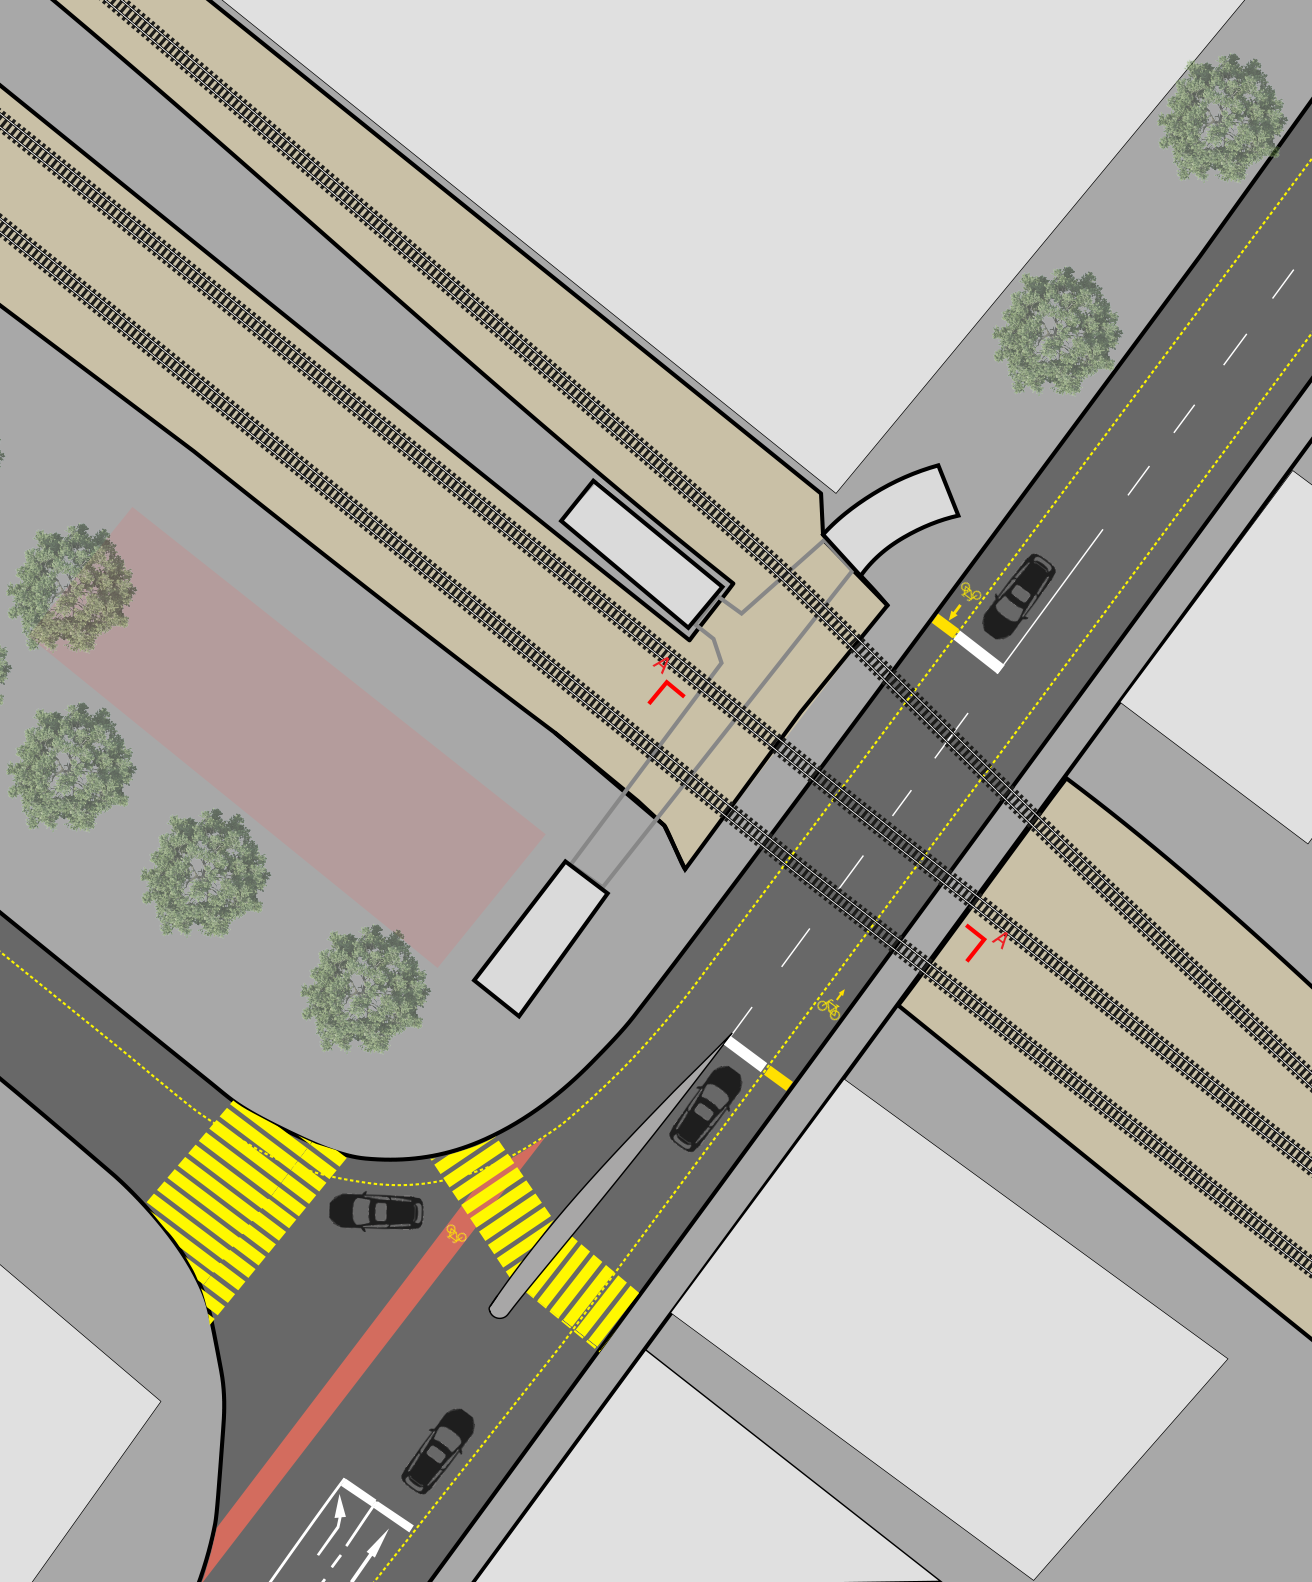
\includegraphics[width=0.65\textwidth]{figures/f-04-05-01-a-V1}
	\caption[Übersicht Variante 1]{Übersicht der Variante 1}
	\label{img:V1Ü}
\end{figure}

\pagebreak

Um die Verkehrssicherheit der Langsamverkehrsteilnehmer minimal zu erhöhen, ist die Anbringung zweier Velostreifen à je 1.5 Meter Breite geplant. Die angenommene maximale Kapazität der beiden Velostreifen zusammen beträgt 3350 Velos pro Stunde. \\
Die Anbringung der Velostreifen erfordert eine geringfügige Verjüngung der Fahrbahn von 4 auf 3.5 Meter pro Fahrbahn. Trotz Verjüngung wird angenommen, dass der zweispurige Strassenabschnitt (eine pro Richtung) eine Kapazität von 2'500 Fahrzeugen pro Stunde aufweist, bei einer geplanten, zulässigen Höchstgeschwindigkeit 50 $km/h$. Unter Berücksichtigung der Situation vor Ort wird angenommen, dass die durchschnittlich gefahrene Geschwindigkeit des MIV 37 $km/h$ beträgt und die der Velofahrer durchschnittlich 15 $km/h$. \\ (\cite{Nacto2018}) (\cite{Mikrozensus2015})

\begin{figure}[h!]
	\centering
	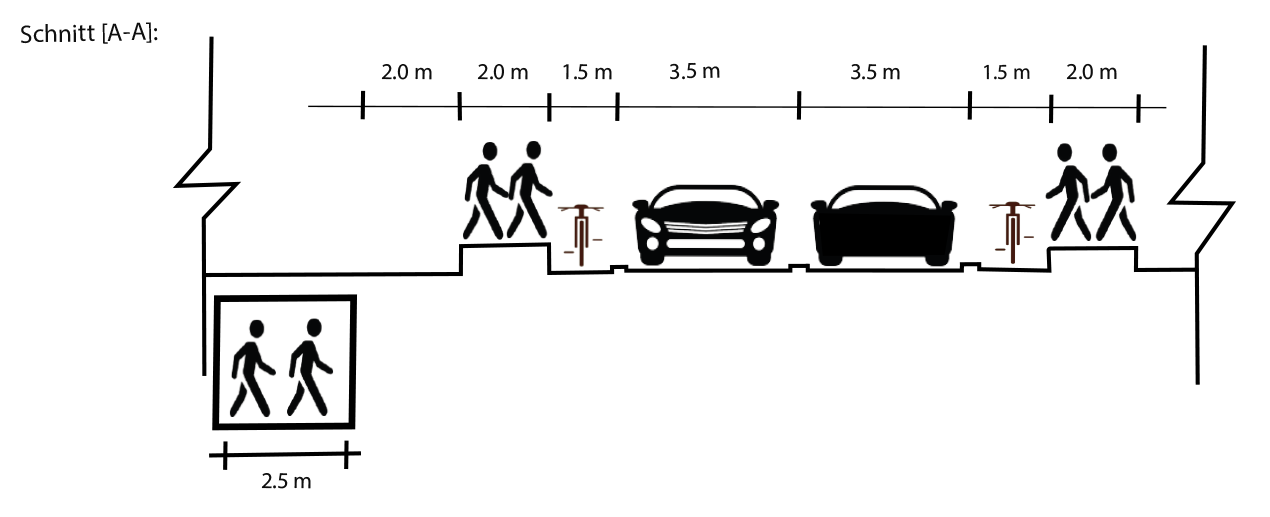
\includegraphics[width=0.7\textwidth]{figures/f-04-05-01-b-V1}
	\caption[Querschnitt Variante 1]{Querschnitt im Schnitt A-A der Variante 1}
	\label{img:V1Q}
\end{figure}

Die Erstellung zweier neuer Radstreifen à je 1.5 Meter Breite kostet gemäss Abschnitt \ref{sub:Unterhalt} 850 CHF pro Laufmeter. Bei einer Gesamtlänge von 80 Meter ergibt sich für den Bau der Variante 1 Kosten im Bereich von 68'000 CHF. (\cite{Baukosten2010}) 

\pagebreak

\subsection{Variante: \ 2}
\label{subsec:V2}
	
Die zweite Variante beinhaltet, wie in Abbildung \ref{img:V2Ü} ersichtlich, den Bau von zwei Velounterführungen, um die lange Wartezeit am Bahnübergang zu verkürzen. Für die Velofahrer entsteht in dieser Variante demnach nur der Zeitverlust gemäss Abschnitt \ref{sub:Reisezeit}, der aufgrund des Befahrens der Infrastruktur entsteht. Die für den MIV angesetzte durchschnittliche Wartezeit beträgt weiterhin 5'. 

Infolge der Rückklassierung der Brunnenstrasse wird ein Tempo 30 Regime eingeführt. Die angenommene durchschnittlich gefahrene Geschwindigkeit des MIV beträgt somit 30 $km/h$ und für die Velofahrer wird angenommen, dass sie mit durchschnittlich 20 $km/h$ durch die Unterführung fahren können. \\ (\cite{Mikrozensus2015})

%\begin{figure}[h!]
 % \centering
 % \subfloat[][]{\label{img:V2Ü}\includegraphics[width=.6\textwidth]{./figures/2}}
  %\hfill
 % \subfloat[][]{\label{img:V2Q}\includegraphics[width=.4\textwidth]{./figures/2_2}}
%\caption[Variante 2]{Übersicht und Querschnitt der Variante 2}
  %\label{fig:V2}
%\end{figure}

\begin{figure}[h!]
	\centering
	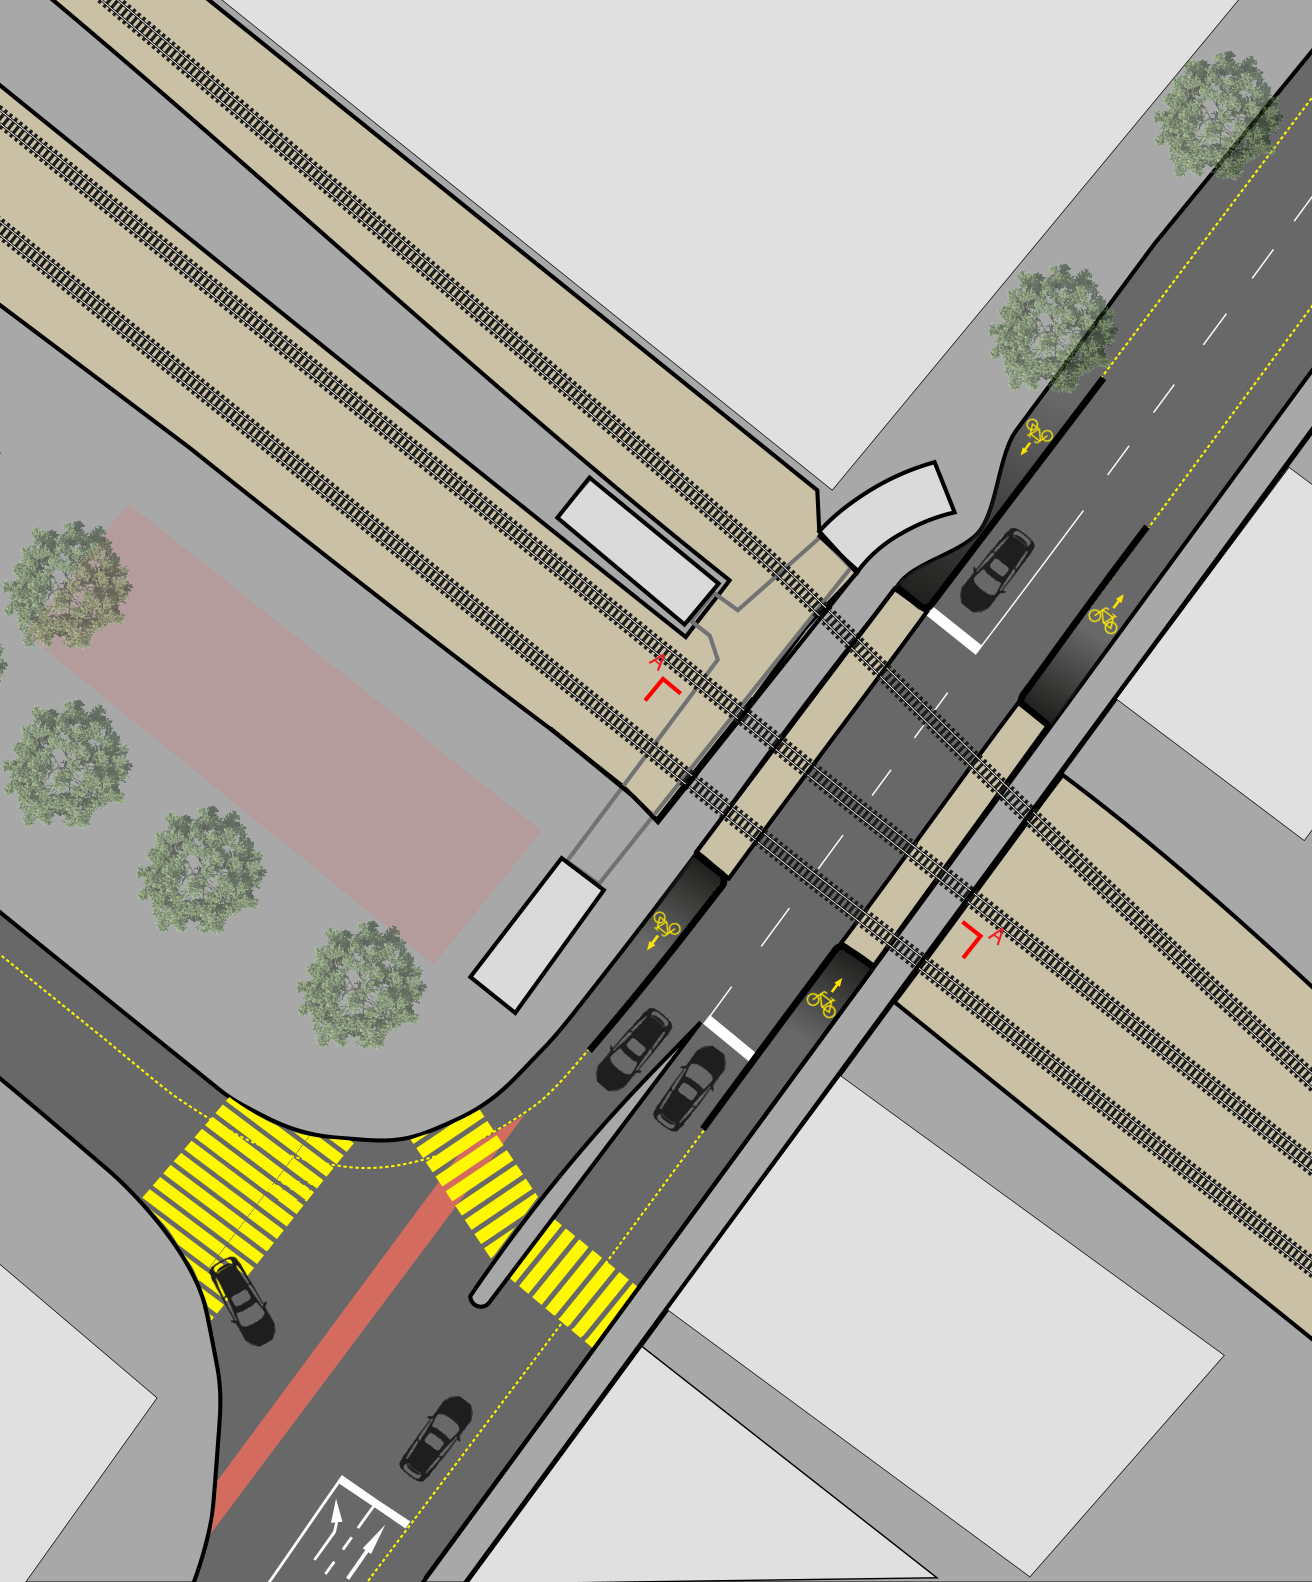
\includegraphics[width=0.65\textwidth]{figures/f-04-05-02-a-V2}
	\caption[Übersicht Variante 2]{Übersicht der Variante 2}
	\label{img:V2Ü}
\end{figure}

Durch den Bau der beidseitig mit einer lichten Breite von 1.5 Meter ausgeführten Velounterführungen, wird einerseits die Verkehrssicherheit der Velofahrer verbessert und andererseits die Kapazität der gesamten Veloinfrastruktur auf maximal 3767 Velos pro Stunde erhöht. Die Gesamtlänge einer Unterführung beträgt in dieser Variante 55 Meter. 
Um diese Unterführung bauen zu können, ist eine weitere Verjüngung der Fahrbahn auf 3 Meter erforderlich, was jedoch zu keiner Reduktion der Kapazität des MIV führen wird.  \\ (\cite{Nacto2018})

\begin{figure}[h!]
	\centering
	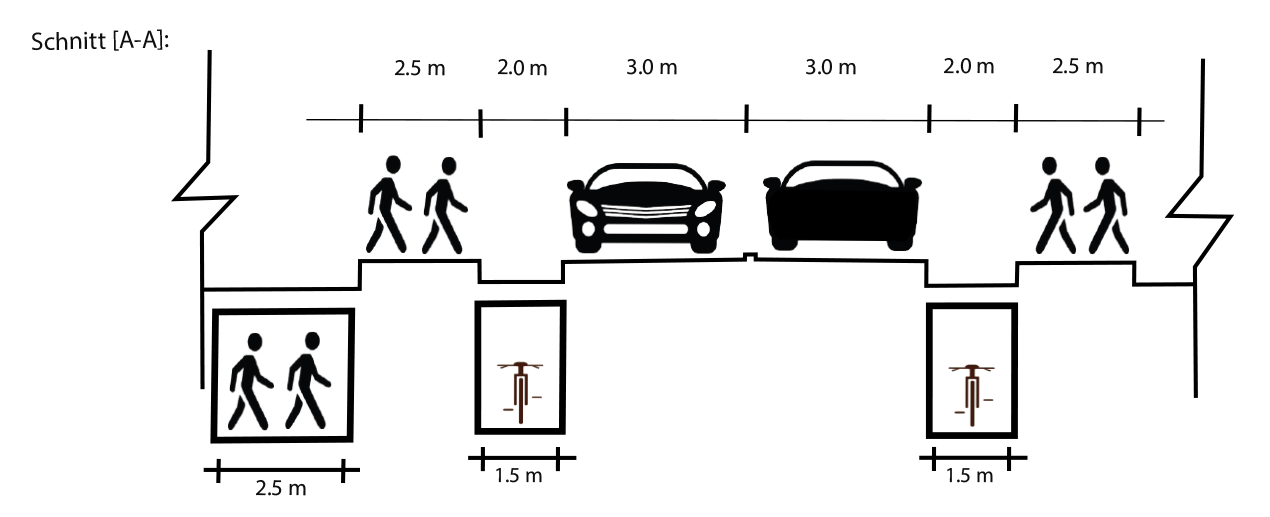
\includegraphics[width=0.7\textwidth]{figures/f-04-05-02-b-V2}
	\caption[Querschnitt Variante 2]{Querschnitt im Schnitt A-A der Variante 2}
	\label{img:V2Q}
\end{figure}

Die prognostizierten Baukosten der Variante 2 werden mithilfe der in Abschnitt \ref{sub:Unterhalt} erläuterten Einheitskosten für den Bau einer Velounterführung und den vorgängig erwähnten Abmessungen der Unterführungen berechnet. Die zu erwartenden Baukosten belaufen sich auf 1.16 Mio. CHF, wobei 520'000 CHF für die vier Rampen und 640'000 CHF für den Bau der Unterführungen unter dem Lastfall Eisenbahn sowie das Anbringen der Velostreifen anfallen. (\cite{Baukosten2010}) 

\pagebreak

\subsection{Variante: \ 3}
\label{subsec:V3}

Die dritte Variante habe ich ausgehend von der Variante 2 entwickelt und ist ein Versuch die Verkehrssicherheit sowie den Fahrkomfort für die Velofahrer zu steigern. Um dies zu erreichen, wird, wie in Abbildung \ref{img:V3Ü} ersichtlich, die Velounterführung zweispurig ausgeführt, was zur Folge hat, dass die Strasse einspurig über den Bahnübergang geführt werden muss. Diese Strassenführung erfordert die Einführung eines Ampelsystems, was die durchschnittliche Wartezeit für den MIV, bei einem Rotlichtzyklus von einer Minute, auf 7 Minuten erhöht. Für das Ampelsystem wäre zusätzlich eine Busbevorzugungsanlage zu prüfen. \\

Die maximale Höchstgeschwindigkeit beträgt wie in Variante 2 30 $km/h$, wobei angenommen wird, dass die Velofahrer mit bis zu 30 $km/h$ durch die Unterführung fahren könnten. (\cite{Mikrozensus2015})

%\begin{figure}[h!]
 % \centering
  %\subfloat[][]{\label{img:V3Ü}\includegraphics[width=.6\textwidth]{./figures/3}}
  %\hfill
 % \subfloat[][]{\label{img:V3Q}\includegraphics[width=.4\textwidth]{./figures/3_2}}
%\caption[Variante 3]{Übersicht und Querschnitt der Variante 3}
 % \label{fig:V3}
%\end{figure}

\begin{figure}[h!]
	\centering
	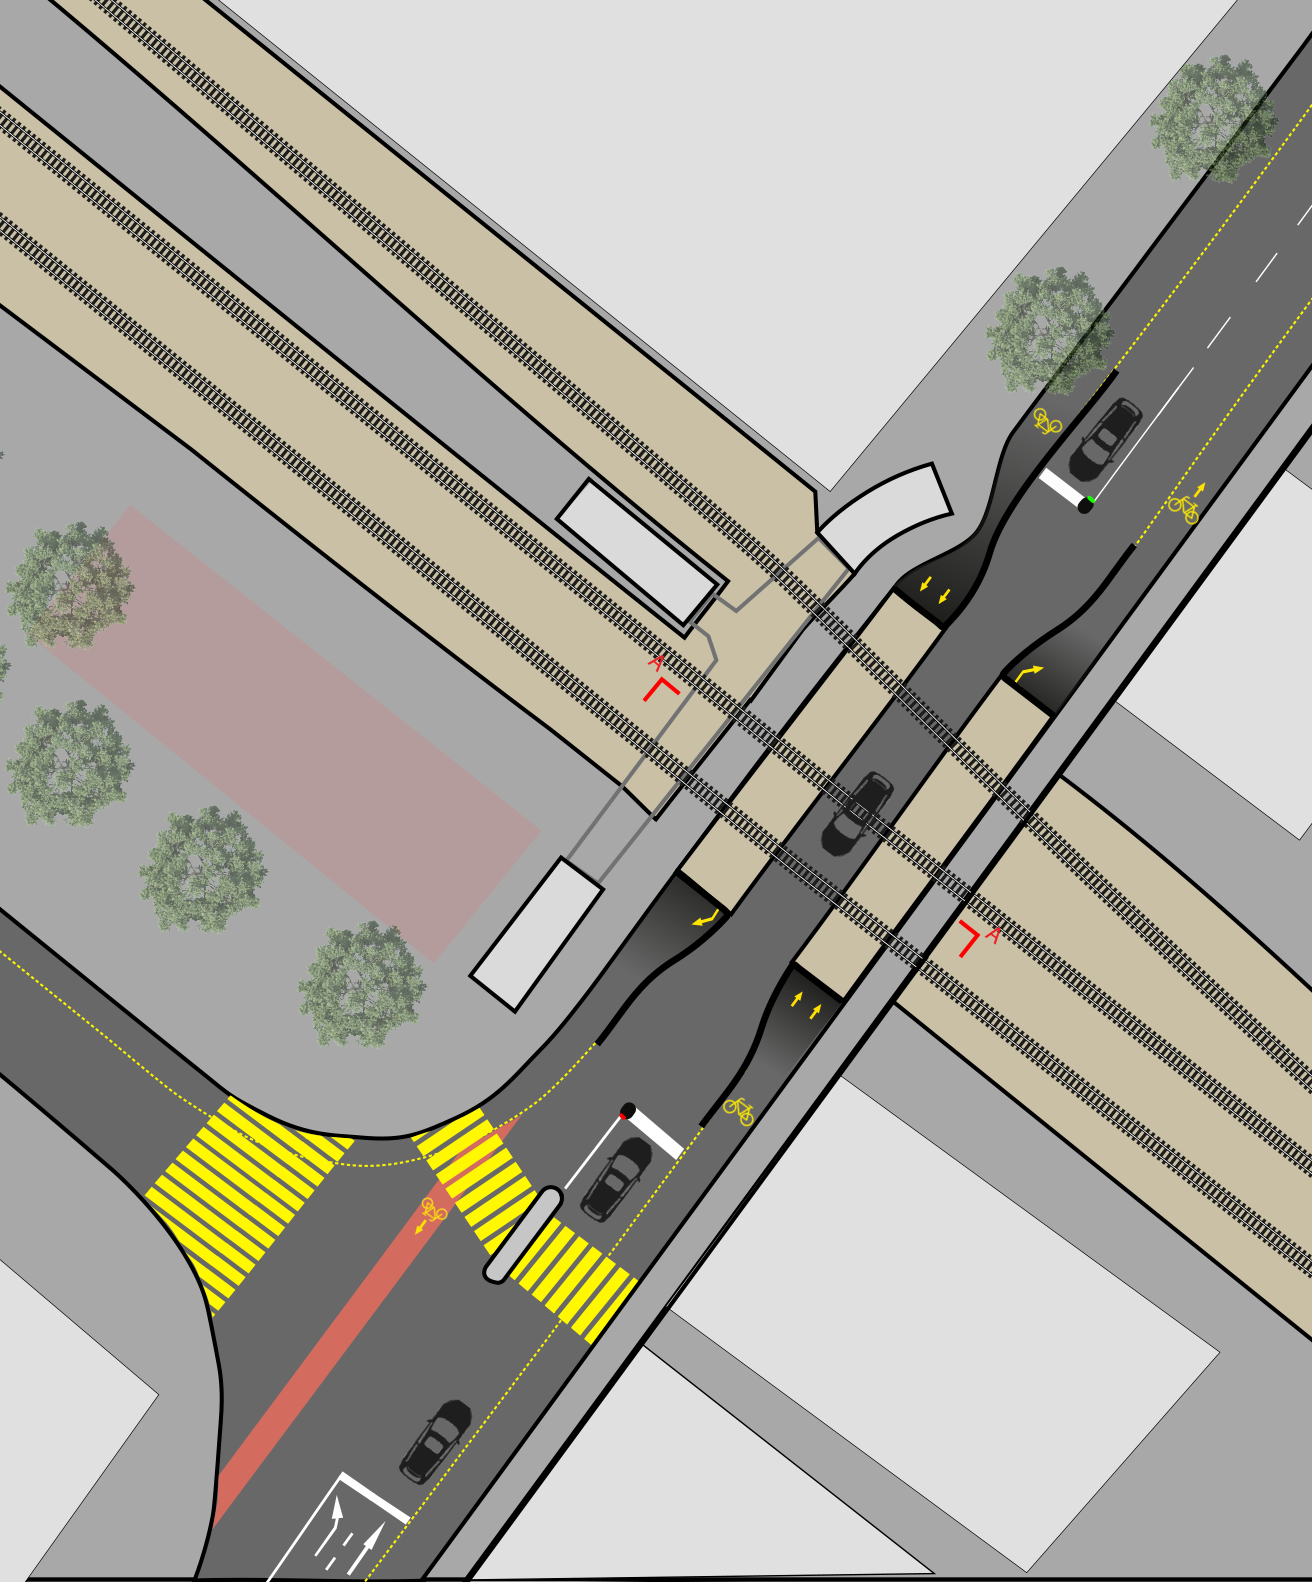
\includegraphics[width=0.65\textwidth]{figures/f-04-05-03-a-V3}
	\caption[Übersicht Variante 3]{Übersicht der Variante 3}
	\label{img:V3Ü}
\end{figure}

Die lichte Breite der Velounterführung beträgt 2 Meter und die Gesamtlänge einer Unterführung beläuft sich auf 65 Meter. Die zweispurige Strassenführung wird mit Fahrbahnmarkierungen verdeutlicht. Es wird angenommen, dass durch diese Ausführung die Kapazität der gesamten Veloinfrastruktur auf maximal 4600 Velos pro Stunde erhöht wird. \\(\cite{Nacto2018})

Infolge der Reduktion der Strasseninfrastruktur um eine Spur nehme ich, dass sich die Kapazität auf 1'250 Fahrzeuge pro Stunde halbiert. Die Fahrspur bleibt mit 5 Meter für grosse Busse weiterhin problemlos befahrbar.

\begin{figure}[h!]
	\centering
	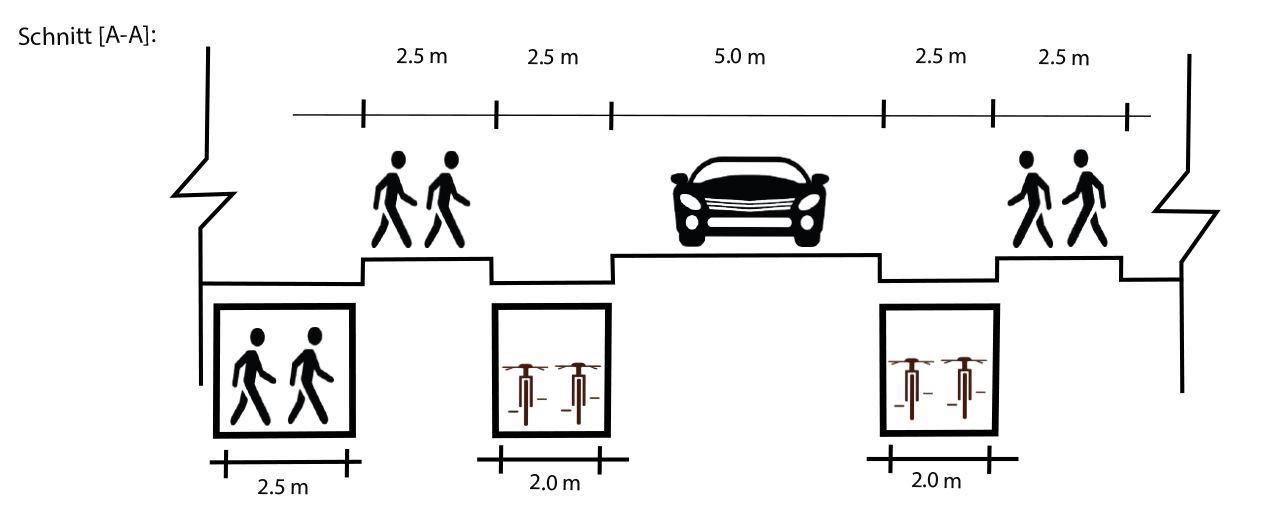
\includegraphics[width=0.7\textwidth]{figures/f-04-05-03-b-V3}
	\caption[Querschnitt Variante 3]{Querschnitt im Schnitt A-A der Variante 3}
	\label{img:V3Q}
\end{figure}

Die Baukosten der Variante 3 belaufen sich auf insgesamt 1.51 Mio. CHF und werden wie für Variante 2 berechnet. Für den Bau der Unterführung unter dem Lastfall Eisenbahn und das Anbringen der Velostreifen sind 988'000 CHF vorgesehen und für den Bau der vier Rampen fallen 520'000 CHF an. \\ (\cite{Baukosten2010}) 


In Tabelle \ref{tab:t-08-01-Varianten} werden die, für die Berechnung der Kosten verwendeten Eigenschaften der Varianten zusammengefasst.
%=============================================================================
% Thesis Template in LaTex
%
% File:  t-05-01-IsingModel.tex -- Table for the Ising
% Author(s): Juergen Hackl <hackl@ibi.baug.ethz.ch>
%            Clemens Kielhauser <kielhauser@ibi.baug.ethz.ch>
%
% Creation:  27 Jan 2014
% Time-stamp: <Tue 2013-08-13 20:14 juergen>
%
% Copyright (c) 2014 Infrastructure Management Group (IMG)
%               http://ibi.ethz.ch
%
% More information on LaTeX: http://www.latex-project.org/
%=============================================================================
%\small\renewcommand{\arraystretch}{1.2} 
%


\begin{table}[h!]
\scriptsize
{\setstretch{0.6}
%\renewcommand{\arraystretch}{1.4}
\flushleft
\begin{tabular}{@{}p{5cm} p{2.5cm} p{2.5cm} p{2.5cm}@{}} \\   
\toprule 		
\textbf{Eigenschaften}  				   								&\textbf{Variante\,1}  & \textbf{Variante\,2} & \textbf{Variante\,3}   \\			
\midrule 
Länge Fahrbahn ($m$)         	 		   								& 80                    & 80    			   & 80             	\\
Länge Unterführung ($m$)       	 		   								& -                     & 55    			   & 65             	\\
Velospuren:					   											&  2				    &  2				   &  4         		\\
Fahrbahnen									 		   					&  2				    &  2				   &  1         		\vspace*{0.25mm} \\
Breite eines Veloweg ($m$):				   								&  1.5				    &  1.5				   &  2         		\\
Breite einer Fahrbahn ($m$):			 		   					    &  3.5				    &  3				   &  5         		\vspace*{0.25mm} \\
Tempolimit	($\frac{km}{h}$) 		   						    		& 50				    & 30				   & 30                	\\
\underline{$\varnothing$\,Geschwindigkeit} ($\frac{km}{h}$) 			&       	            &   				   &               		 \\
\hspace*{5mm}\textbullet\, Velo            		       					& 15  					& 20    			   & 25      			\\
\hspace*{5mm}\textbullet\, MIV            		       					& 37  					& 30    			   & 30      			\vspace*{0.25mm} \\
\underline{Kapazität} ($\frac{Fahrzeug}{h}$)		        			&    				    &  				       &                  	 \\
\hspace*{5mm}\textbullet\, Velo            	       					    & 3350 					& 3767    			   & 4600      			\\
\hspace*{5mm}\textbullet\, MIV         		       					    & 2500 					& 2500    			   & 1250      			\\
\underline{Wartezeit} ($Minuten$)        		    			   		&    				    &  				       &                  	 \\
\hspace*{5mm}\textbullet\, Velo            	       					    & 5 					& 5    			       & 7      			\\
\hspace*{5mm}\textbullet\, MIV         		       					    & 5  					& 0      			   & 0      			\\
Baukosten ($CHF$)														& 68'000				& 1.16 Mio.			   & 1.51 Mio.           \\
\bottomrule

\end{tabular}
\caption{Basis Informationen der Varianten}
\label{tab:t-08-01-Varianten}
}
\end{table}


%=============================================================================
% EOF
%

%%% Local Variables:
%%% mode: latex
%%% TeX-master: "../guidelines"
%%% End:



\pagebreak

% ===========================================================================
% EOF
%

%%% Local Variables:
%%% mode: latex
%%% TeX-master: "../main"
%%% End:


%----------------------

\section{Analyse der Lösungen}
\label{sec:Analyse}

Um den Vergleich der Varianten, zur Bestimmung der optimalen Lösungen, durchführen zu könne, müssen die Kosten anhand der unter Abschnitt \ref{sec:Kostenstruktur} dargestellten Formeln, berechnet werden. Um die Kosten über einen Zeitraum von vierzig Jahren berechnen zu könne, muss der Einfluss der unter Abschnitt \ref{subsec:Uncertain} bestimmten Faktoren, auf das DTV modelliert werden und somit der DTV für die Zukunft geschätzt werden. Dies geschieht anhand der nachfolgend vorgestellten Szenarien.


	\subsection{Modellierung des DTV}
	\label{subsec:Modellierung}
	
Den Effekt der das Bevölkerungswachstum auf den $DTV_{MIV}$ sowie auf den $DTV_{Velo}$ haben wird, untersuche ich anhand der im nachfolgenden Abschnitt \ref{subsubsec:Demographie} dargestellten Szenarien. Den Effekt der die Umsetzung der Leitziele des STEK bis 2035 auf den Langsamverkehr haben wird fasse unter dem Stichpunkt \textit{Umsetzung der STEK} zusammen. Dieser Umfasst die Einflüsse welche die Entwicklung des Zentrums, der Ausbaus der Veloparkieranlage am Bahnhof, die Aufwertung der Quartiere nördlich des Bahnhofs und die Massnahmen der Stadt Uster zur Förderung des Langsamverkehrs, sowie der Ausbaus des Spitals auf den $DTV_{Velo}$ haben werden.

Da diese Effekte zur gleichen Zeit wirken, muss eine bei der Berechnung der Kosten der Varianten eine Kombination der gebildeten Szenarien betrachtet werden. Gemäss des unter Abschnitt \ref{sec:Decisiontree} vorgestellten Entscheidungsbaum und dem Beispiel in Abbildung \ref{img:EntscheidungBSP}, wird dies in der nachfoldenen Abbildung \ref{img:EntscheidunSzenarien} dargestellt. Dies stellt zugleich einen Ausschnit aus dem Entscheidungprozess, zur Bestimmung der optimalen Lösung, dar.

\begin{figure}[h!]
	\centering
	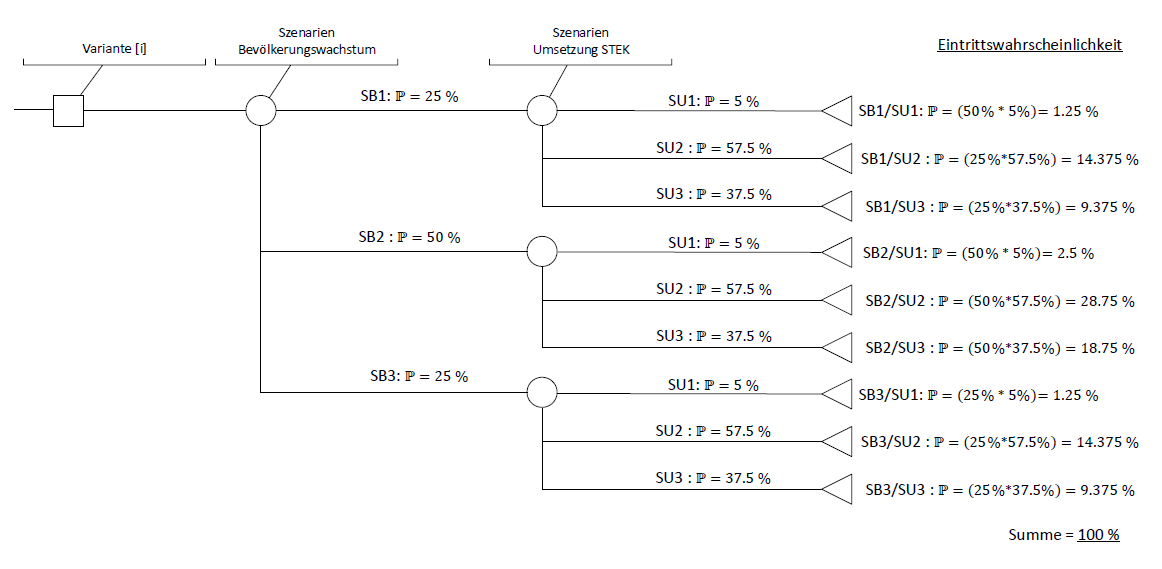
\includegraphics[width=\textwidth]{figures/04-06-01-Entscheidungsbaum-Szenarien}
	\caption[Szenarienübersicht]{Übersicht über die Szenarien und ihre Eintrittswahrscheinlichkeiten}
	\label{img:EntscheidunSzenarien}
\end{figure}

	%=============================================================================
% Thesis Template in LaTex
%
% File:  04-06-Szenarien.tex -- Fallstudie/Modellierung der ungewissen Parameter
% Author(s): Jürgen Hackl <hackl@ibi.baug.ethz.ch>
%            Clemens Kielhauser <kielhauser@ibi.baug.ethz.ch>
%
% Creation:  27 Jan 2014
% Time-stamp: <Tue 2013-08-13 20:14 juergen>
%
% Copyright (c) 2014 Infrastructure Management Group (IMG)
%               http://ibi.ethz.ch
%
% More information on LaTeX: http://www.latex-project.org/
%=============================================================================

% Unterkapitel Szenarien
% ---------

\subsubsection*{Bevölkerungswachstum}
\label{subsubsec:Bevölkerung}

Wie in Kapitel \ref{chap:Fallstudie} erwähnt, ist das DTV mehrheitlich von der zukünftigen demographischen Entwicklung abhängig.
Um den Effekt, den das Bevölkerungswachstum auf das DTV haben wird, modellieren zu können, orientiere ich mich an den Wachstumsprognosen der Stadt Uster.
Die zu erwartende Bevölkerungsentwicklung habe ich dem Kapitel 3 \textit{Stadt Uster im Porträt} des STEK entnommen und wird nachfolgend kurz beschrieben. 

\begin{description}
\item[Stagnation] \hfill \\
Geschätzte Anzahl an Einwohner im Jahr 2035: 38'760 \\
$\Rightarrow$ + 188 Einwohner/Jahr \\ $\Rightarrow$ + 0.5\% pro Jahr gegenüber 2015
\item[Trend restriktiv] \hfill \\
Geschätzte Anzahl an Einwohner im Jahr 2035: 42'260 \\ 
$\Rightarrow$ + 363 Einwohner/Jahr \\ $\Rightarrow$ + 1\% pro Jahr gegenüber 2015
\item[Trend Prosperität] \hfill \\
Geschätzte Anzahl an Einwohner im Jahr 2035: 45'620 \\ 
$\Rightarrow$+ 531 Einwohner/Jahr \\ $\Rightarrow$ + 1.5\% pro Jahr gegenüber 2015
\end{description}

Anhand dieser Wachstumsprognosen und unter der Annahme eines linearen Wachstums, definiere ich die drei nachfolgend dargestellten Szenarien. Mit diesen Szenarien werde ich in einem nächsten Schritt den zukünftigen DTV für den MIV und den Langsamverkehr, sprich Veloverkehr, am Bahnübergang Brunnenstrasse ermitteln.
Ausgehend vom DTV des MIV im Jahr 2016 und den Wachstumsraten der Szenarien habe ich die jährliche Zunahme an Motorfahrzeugen ermittelt. Im Jahr 2016 lag das DTV des MIV am Bahnübergang bei 12'023 Motorfahrzeugen pro Tag. \\ (\cite{GIS})

\begin{itemize}
\item Szenario: SB 1
	\begin{itemize}
	\item Grundlage: Stagnation $\Rightarrow$ jährliches Wachstum um 0.5\%
	\item Jährliche Zunahme DTV: 60 Fahrzeuge
	\item Eintrittswahrscheinlichkeit: 25\%
	\end{itemize}
\item Szenario: SB 2
	\begin{itemize}
	\item Grundlage: Trend restriktiv  $\Rightarrow$ jährliches Wachstum um 1 \%
	\item Jährliche Zunahme DTV: 120 Fahrzeuge
	\item Eintrittswahrscheinlichkeit: 50\%
	\end{itemize}
\item Szenario: SB 3
	\begin{itemize}
	\item Grundlage: Trend Prosperität  $\Rightarrow$ jährliches Wachstum um 1.5\%
	\item Jährliche Zunahme DTV: 180 Fahrzeuge
	\item Eintrittswahrscheinlichkeit: 25\%
	\end{itemize}
\end{itemize}


Die Wahrscheinlichkeit das Szenario SB 2 eintritt und das DTV jährlich um 120 Fahrzeuge zunimmt, bewerte ich mit 50\%. Dies erfolgt unter der Annahme, dass der restriktive Trend das minimale Wachstumsziel von 20\% wiederspiegelt, welches gemäss dem STEK mit grösster Wahrscheinlichkeit eintreten wird, und da dieses Szenario den kantonalen Prognosen entspricht, erachte ich dieses Szenario als das wahrscheinlichste und bewerte es dementsprechend.

Das es zu einem verstärktem Wachstum von 1.5\% und somit zu einer jährlichen Zunahme von 180 Fahrzeugen am DTV kommt, erachte ich nach den Angaben des STEK als unwahrscheinlich, da ein übermässiges Bevölkerungswachstum aufgrund der nur beschränkt vorhandenen Kapazitäten zur Erweiterung der Wohnangebots, nur bedingt möglich ist. 

Das es zu einer Stagnation des Bevölkerungswachstums und im Zuge dieser Modellierung zu einem Verkehrswachstum von 0.5\% und einer jährlichen Zunahme von 60 Fahrzeugen am DTV kommt, erachte ich in Anbetracht der Prognosen zur demographische Entwicklung im Kanton Zürich, als unwahrscheinlich. Deshalb bewerte ich die Szenarien SB 1 und SB 3 mit jeweils 25\%.

Mithilfe der verschiedenen Wachstumsraten $WR_{s}$ der Szenarien und der Formel \ref{eq.11} berechne ich das $DTV_{i}$ im Jahr $t_{i}$. \\
Der DTV des Jahres 2016 lag, wie oben erwähnt, bei 12'023 Motorfahrzeuge pro Tag. Diesen Wert nutze ich als Start- sowie Basiswert meiner Berechnungen. 

\begin{equation}
DTV_{i} = DTV_{2016} + \bigl( t_{i} - t_{2016} \bigr) \cdot \bigl[WR_{s}\bigr] \cdot DTV_{2016}
\label{eq.11}
\end{equation}

Da die Anzahl Velos, die den Bahnübergang Brunnenstrasse täglich passieren, nicht von einer Verkehrsmessstelle gezählt werden, muss diese Information aus dem MIV hergeleitet werden. Dies erfolgt mithilfe der Daten der Verkehrsmessstelle an der etwas südlich von Uster gelegenen Seefeldstrasse, welche Niederuster mit Riedikon verbindet. 
Der im Jahr 2019 gemessen durchschnittliche DTV lag bei 8818 Motorfahrzeugen für das MIV und 913 Velos. Daraus ergibt sich einen Veloanteil von 10.35\%. \footcite{MIVSeefeld}\footcite{VeloSeefeld}

\begin{align*}
\mu &= \frac{DTV_{Velo,Seefeldstrasse}}{DTV_{MIV,Seefeldstrasse}}   \\[2ex]
DTV_{Velo} &= DTV_{MIV} \cdot \mu_{Velo} 
\end{align*}

In den Abbildung \ref{fig:DTV} sind die Ergebnisse meiner Modellierung des DTV am Bahnübergang Brunnenstrasse dargestellt, die ich für die Berechnung der Kosten der Varianten verwenden werde. Eine ausführliche Tabelle aller modellierten DTV-Werte findet sich unter Abschnitt \ref{subsec:DTVModellierung}

\begin{figure}[h!]
  \centering
  \subfloat[][]{\label{fig:04-06-02-DTV(MIV)}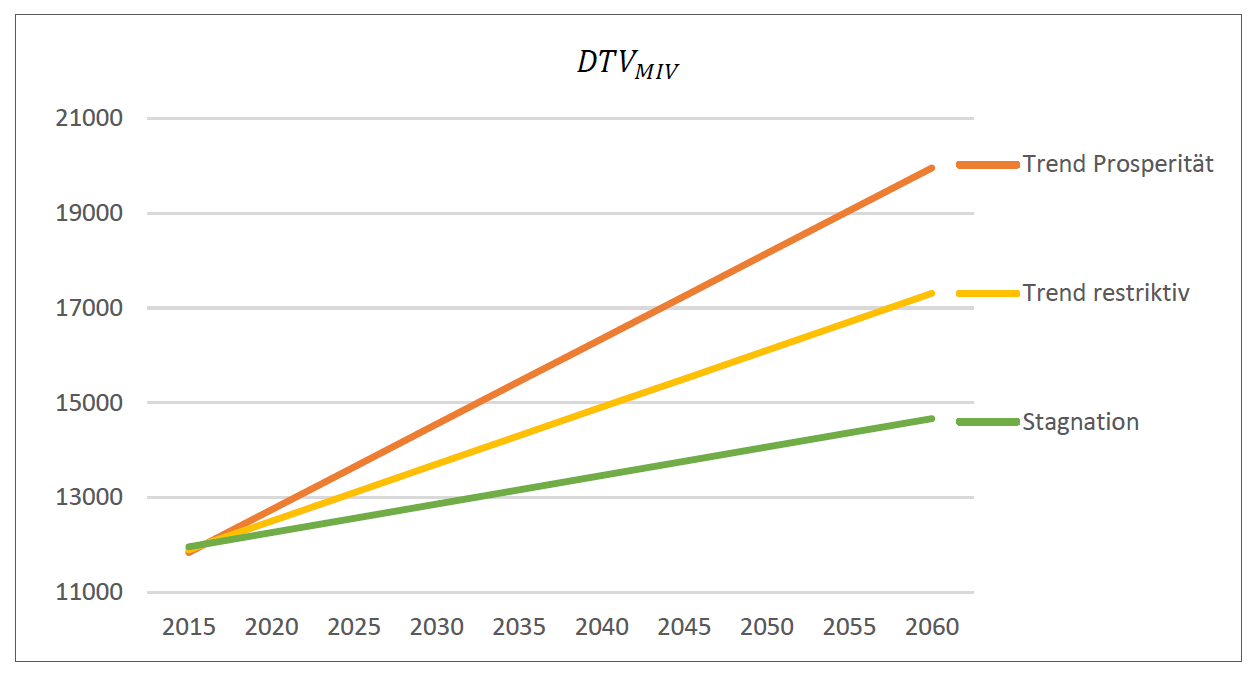
\includegraphics[width=.5\textwidth]{./figures/f-04-06-02-DTV(MIV)-SzenarienBev-Wachstum}}
  \hfill
  \subfloat[][]{\label{fig:04-06-03-DTV(VELO)}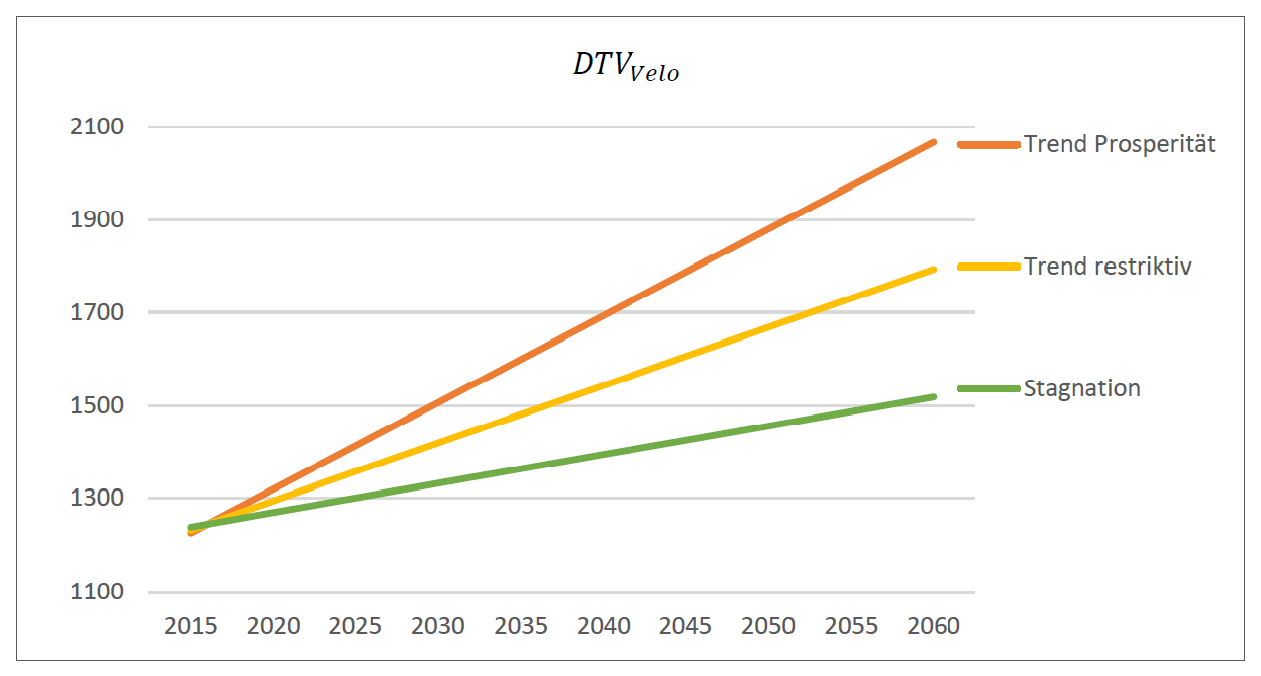
\includegraphics[width=.5\textwidth]{./figures/f-04-06-03-DTV(VELO)-SzenarienBev-wachstum}}
\caption[DTV Brunnenstrasse]{DTV an der Brunnenstrasse}
  \label{fig:DTV}
\end{figure}



\subsubsection*{Umsetzung STEK}
\label{subsubsec:Umsetzung}

Die folgenden Szenarien modellieren die Effekte, den die in Abschnitt \ref{subsec:Modellierung} unter dem Stickwort \textit{Umsetzung STEK} zusammengefassten Einflussfaktoren, auf den $DTV_{Velo}$ haben werden. 

Das meines Erachtens mit grösster Wahrscheinlichkeit eintretende Szenario entspricht der Verkehrsprognose des Bundes, die eine Zunahme der Verkehrsleistung des Langsamverkehrs bis 2040 gegenüber 2010, um 32\% erwartet. (\cite{Perspektive2040}) 

Um die Ober- sowie Untergrenze meiner Prognose ermitteln zu können, orientiere ich mich ein weiteres Mal am STEK. Mithilfe der unter Kapitel 10 \textit{Stadt Uster im Porträt} des STEK vorgestellten Wachstumsprognosen für die Bevölkerungsentwicklung sowie der in Kapitel 7 \textit{Mobilität} des STEK gemäss regionalem Richtplan erstellten Verkehrsprognose für den Anteil der Velofahrer am Gesamtverkehr, erstelle ich zwei weitere Szenarien. 
Einerseits berücksichtige ich den Fall einer ungenügenden Umsetzung der Leitziele und der daraus resultierenden stagnierenden Entwicklung des Veloverkehrs. Andererseits den Fall einer maximalen Umsetzung aller Ziele in Verbindung mit einer Verschiebung des Innerstädtischen Modalsplit in Richtung Langsamverkehr.

\pagebreak

\begin{description}
\item[Stagnation] \hfill \\
Prognose gemäss STEK: $\Rightarrow$ jährliches Wachstum: 0.54 \% 
\item[Verkehrsperspektiven 2040] \hfill \\
Prognostizierte Zunahme der Verkehrsleistung: 32\% $\Rightarrow$ jährliches Wachstum: 1.3 
\item[Umsetzung maximal] \hfill \\
Prognose gemäss STEK und regionalem Richtplan: $\Rightarrow$ jährliches Wachstum: 2 \% 
\end{description}

Eine Stagnation erachte ich unter Berücksichtigung der Entwicklung des Langsamverkehrs über die letzten zehn Jahre, als unwahrscheinlich und bewerte das Eintreten dieser Prognose demzufolge mit 5\%. \\
Dass es zu einem Wachstum gemäss der Prognose des Bundes kommen wird, erachte ich nach der Konsultation weitere Verkehrsprognosen, als das Szenario, welches mit grösster Wahrscheinlichkeit eintreten wird. Daher bewerte ich dieses Szenario mit einer Eintrittswahrscheinlichkeit von 57.5\%. \\
Dass alle Ziele maximal erfüllt werden und eine Verschiebung des innerstädtischen Modal-Split stattfindet, erachte ich mit 32.5\% als deutlich plausibler als die Stagnation, jedoch als unwahrscheinlicher als die Prognose des Bundes. 

\begin{itemize}
\item Szenario: SU 1
	\begin{itemize}
	\item Grundlage: Stagnation 
	\item Eintrittswahrscheinlichkeit: 5\%
	\end{itemize}
\item Szenario: SB 2
	\begin{itemize}
	\item Grundlage: Verkehrsperspektiven 2040
	\item Eintrittswahrscheinlichkeit: 57.5\%
	\end{itemize}
\item Szenario: SB 3
	\begin{itemize}
	\item Grundlage: Umsetzung maximal
	\item Eintrittswahrscheinlichkeit: 32.5\%
	\end{itemize}
\end{itemize}

Anhand der zu Beginn dieses Abschnitts definierten Wachstumsraten, sowie ausgehend von den Messwerten des täglichen Veloverkehrs im Jahr 2016, habe ich die Anzahl Velos, die in jedem Szenario zusätzlich pro Tag auf der Infrastruktur unterwegs sein werden, ermittelt. 
Die Anzahl Velos die im Jahr 2016 täglich den Bahnübergang nutzten, lag, gemäss Abschnitt \ref{subsubsec:Bevölkerung}, bei 1245.

Das Szenario SU 1 führt somit zu einer Erhöhung des täglichen Veloverkehrs um 7 Velos pro Jahr, das Szenario SU 2 zu einer Zunahme von 16 Velos pro Jahr und das Szenario SB 3 zu einer Erhöhung des $DTV_{Velo}$ um 25 Velos pro Jahr. 
Mit diesen Angaben berechne ich die Anzahl Velos, die je nach Szenario, zusätzlich zu den in Abschnitt \ref{subsubsec:Bevölkerung} berechneten DTV-Werten, auf der Infrastruktur unterwegs sein werden.

\pagebreak

% ===========================================================================
% EOF
%

%%% Local Variables:
%%% mode: latex
%%% TeX-master: "../main"
%%% End:



	\subsection{Berechnung der Kosten der Varianten}
	\label{subsec:Kostenberechnung}
	%=============================================================================
% Thesis Template in LaTex
%
% File:  04-07-Kosten -- Analyse der Lösungen - Fallstudie
% Author(s): Jürgen Hackl <hackl@ibi.baug.ethz.ch>
%            Clemens Kielhauser <kielhauser@ibi.baug.ethz.ch>
%
% Creation:  27 Jan 2014
% Time-stamp: <Tue 2013-08-13 20:14 juergen>
%
% Copyright (c) 2014 Infrastructure Management Group (IMG)
%               http://ibi.ethz.ch
%
% More information on LaTeX: http://www.latex-project.org/
%=============================================================================

% Unterkapitel Kosten
% ---------

Die Berechnung der Kosten der Varianten erfolgt ahand der Berchnung der Zielfunktion über den Zeitraum von 40 Jahren. In Abbildung \ref , wird für die Variante 1 im Szenario SB1/SU1, die Berechnung der ersten 5 Jahre gezeigt. Zur Übersicht zeige ich die Formel der Zielfunktion hier erneut. 

\begin{equation*}
Min. \thinspace TK_{i} = Min. \thinspace [K_{U}^i + K_{B}^i + K_{TT}^i + K_{E}^i + K_{A}^i]
\end{equation*} 

Was man im Excell sieht:

-> DTV die ich in mit den im vorangegangenen Abschnitt erläuterten Szenarien ermittelt habe.

Mit excell beispiel File... gemäss MA BSP

Was genau mache ich:
-Berechnung der Zielfunktion über den betrachteten Zeithorizont
-Darstellen der Szenarien mit ihren Eintrittswahrscheinlichkeiten
-Kombination der berechneten Kosten mit den Eintrittswahrscheinlichkeiten -> ergibt die Risiken der Varianten
-Summe aller Risiken ergibt das Risiko der Variante selbst.

% ===========================================================================
% EOF
%

%%% Local Variables:
%%% mode: latex
%%% TeX-master: "../main"
%%% End:


%---------------------

\section{Bewertung der Lösungen}
\label{sec:Bewertung}

Die im vorangegangen Abschnitt berechneten Kosten der Varianten sind abhängig vom jeweiligen Szenario. Da die 

Gewichtung der Szenarien mit dem Eintrittswahrscheinlichkeit...

	\subsection{Berechnung der Risiken der Varianten}
	%=============================================================================
% Thesis Template in LaTex
%
% File: 04-08-Risiken - Bewertung der Lösung -- Fallstudie
% Author(s): Jürgen Hackl <hackl@ibi.baug.ethz.ch>
%            Clemens Kielhauser <kielhauser@ibi.baug.ethz.ch>
%
% Creation:  27 Jan 2014
% Time-stamp: <Tue 2013-08-13 20:14 juergen>
%
% Copyright (c) 2014 Infrastructure Management Group (IMG)
%               http://ibi.ethz.ch
%
% More information on LaTeX: http://www.latex-project.org/
%=============================================================================

% Unterkapitel Risikenberechnung 
% ---------
\label{subsec:BerechnungRisiken}


Wie im vorangegangen Abschnitt erwähnt, berechnet sich das Risiko einer Varianten in einem Szenario, durch die Multiplikation der Eintrittswahrscheinlichkeit des Szenarios mit den für die jeweilige Variante, im betrachteten Szenario, berechneten Kosten. Das Gesamtrisiko das von der Durchführung einer Variante ausgeht, setzt sich somit aus der Summe aller Risiken einer Variante zusammen. 
Anhand der nachfolgenden Abbildung wird als Beispiel die Berechnung des Risiko der Variante 1, mithilfe eines Entscheidungsbaums gezeigt. Die Berechnung erfolgt in diesem Fall von Rechts nach Links.


\begin{figure}[h!]
	\centering
	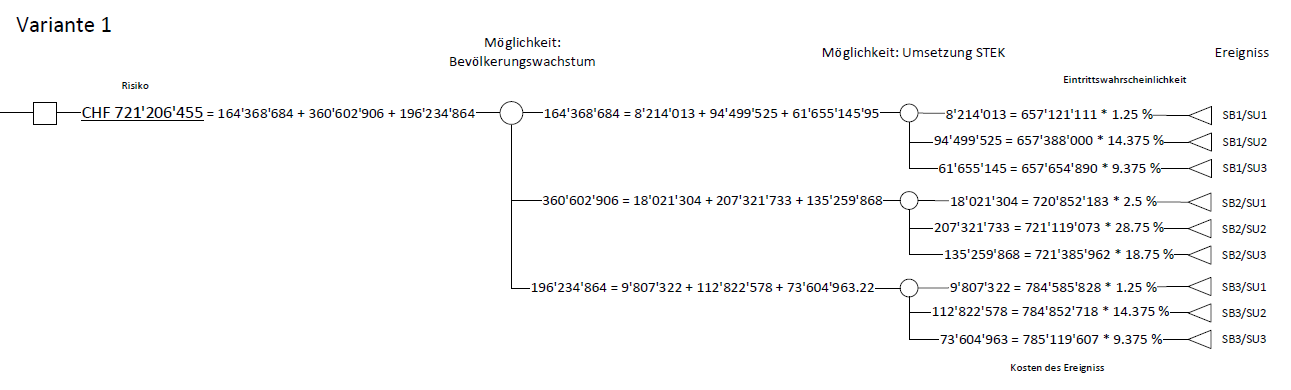
\includegraphics[width=\textwidth]{figures/f-04-08-01-Risikoberechnung}
	\caption[Risikoberechnung]{Beispiel der Risikoberechnung}
	\label{img:Risikoberechnung}
\end{figure}




% ===========================================================================
% EOF
%

%%% Local Variables:
%%% mode: latex
%%% TeX-master: "../main"
%%% End:




	\subsection{Sensitivitätsanalyse}
	\input{content/Fallstudie/04-09-Sensitivitätsanalyse}

% ===========================================================================
% EOF
%

%%% Local Variables:
%%% mode: latex
%%% TeX-master: "../main"
%%% End:


% Chapter 5
% ---------
%=============================================================================
% Thesis Template in LaTex
%
% File:  05-Resultate.tex -- Resultate
% Author(s): Cyrano Golliez <golliezc@student.ethz.ch>
%
% Creation:  27 Jan 2014
% Time-stamp: <Tue 2013-08-13 20:14 juergen>
%
% Copyright (c) 2014 Infrastructure Management Group (IMG)
%               http://ibi.ethz.ch
%
% More information on LaTeX: http://www.latex-project.org/
%=============================================================================

\chapter{Resultate}
\label{chap:Resultate}

Um die Verkehrssituation am Bahnübergang Brunnenstrasse nachhaltig zu verbessern, bedarfs es einer optimalen Variante, die durch den Vergleich der gemäss Abschnitt > berechneten Risiken der Varianten bestimmt wird. Der Vergleich der Risiken der Varianten erfolgt für die in Abschnitt < definierten Zustände um die gefunden optimale Lösung zu bestärken oder allenfalls zu verwerfen.
Nachfolgend dargestellt sind die Resulatet der Risikoberechnung sowie der Risikovergleich und die für die verschiedenen Zustände bestimmte optimale Variante. 

\begin{figure}[h!]
  \centering
  \subfloat[][]{\label{img:RisikoVar-Z0)}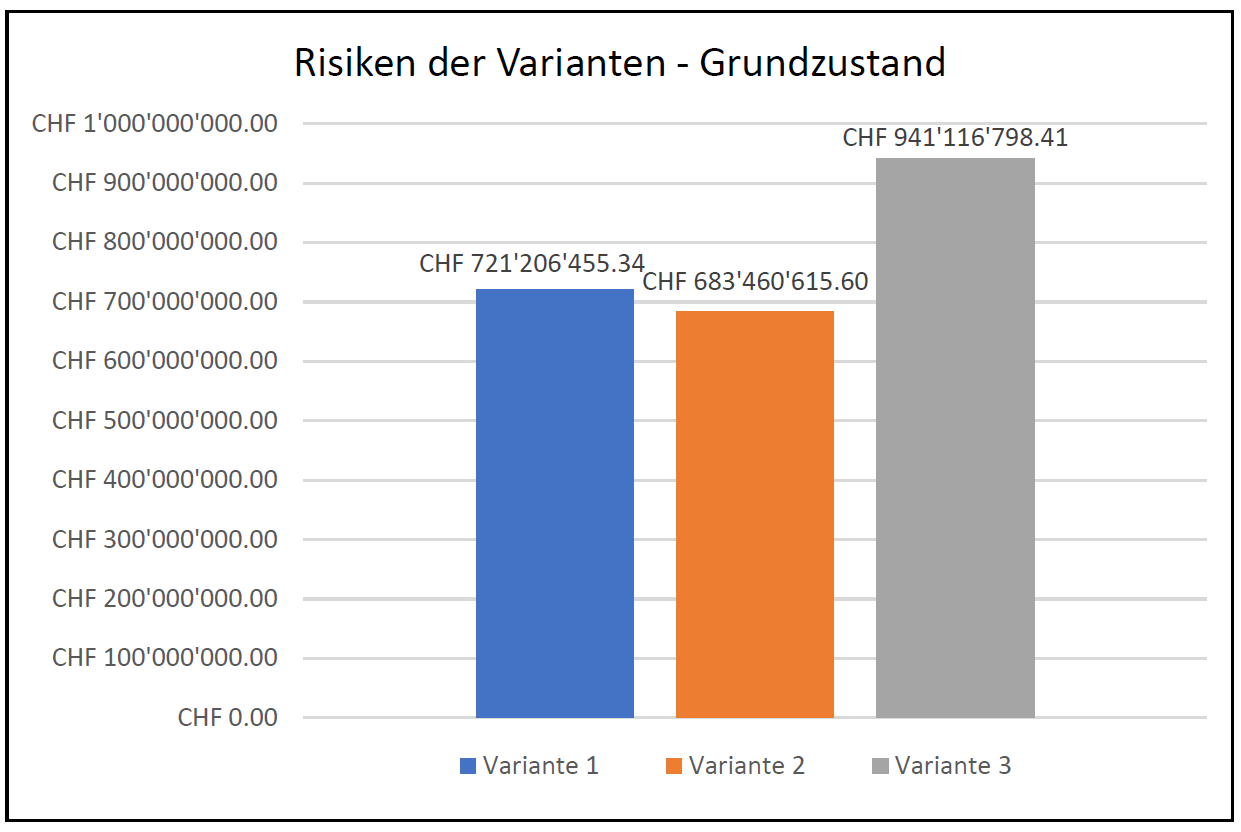
\includegraphics[width=.45\textwidth]{./figures/f-05-02-RisikenVarianteZ0}}
  \hfill
  \subfloat[][]{\label{img:VariantenwahlZ0)}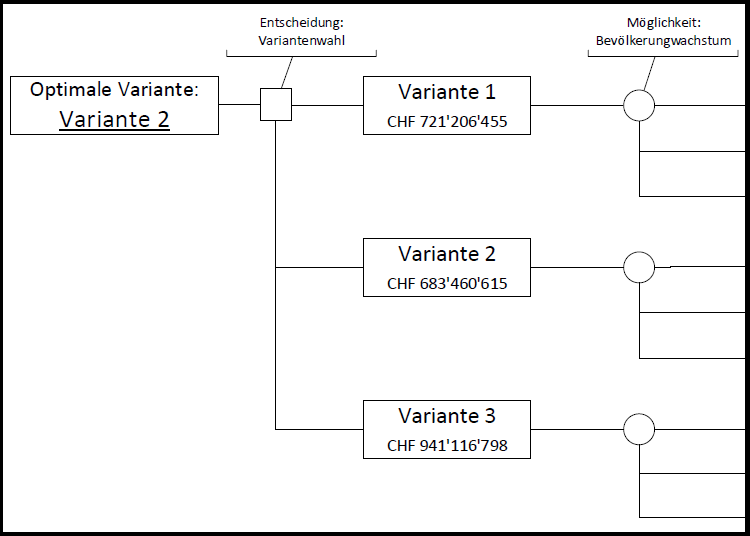
\includegraphics[width=.45\textwidth]{./figures/f-05-01-Variantenwahl}}
\caption[Verkehrsaufkommen]{Risikovergleich und Entscheidungsprozess im Zustand 0}
  \label{fig:Z4}
\end{figure}

\paragraph{Zustand 0}

Wie in der Abbildung \ref{img:RisikovergleichVarianten} ersichtlich, beträgt das Risiko der Variante 1 im Zustand 0 721'206'455 CHF, das Risiko der Variante 2 683'460'615 CHF und das Risiko der Variante 3 941'116'798 CHF. Das Risiko der Variante 2 ist somit um 37'745'840 CHF geringer als das Risiko der Variante 1 und um 257'656'183 CHF kleiner als das Risiko der Variante 3. Die Differenz der Risiken der Varianten 1 und 3 beträgt 219'910'343 CHF. \\
Die Variante mit dem geringsten Risiko im Zustand 0 ist demnach Variante 2 und ist dementsprechen die optimale Variante, wie in Abbildung \ref{img:VariantenwahlZ0} dargestellt.

\paragraph{Zustand 1 bis 3}

Die nachfolgende Abbildung stellt die Risiken der Varianten in den Zuständen 1 bis 3 dar. Es ist klar ersichtlich, dass sich in den Zuständen 1 bis 3 keine Veränderung der optimalen Lösung ergibt und weiterhin die Variante 2 die optimale Lösung darstellt. Aus diesem Grund verzichte ich auf die ausführliche Darstellung der Zustände 1 bis 3 und verweise auf den Abschnitt \ref{chap:Diskussion} in dem ich die Zustände vergleiche und diskutiere.

\begin{figure}[h!]
	\centering
	\includegraphics[width=\textwidth]{figures/f-05-00-01-RisikenVergleichZustände1-3}
	\caption[Risikovergleich der Zustände 1 bis 4]{Risiken der Varianten - Vergleich der Zustände 1 bis 3}
	\label{img:RisikovergleichVarianten}
\end{figure}

\paragraph{Zustand 4}

Im Zustand 4 beträgt das Risiko der Variante 1 wie im Zustand 0 721'206'455 CHF. Das Risiko der Variante 2 beträgt 683'460'616 CHF und das Risiko der Variante 3 ist mit 683'422'520 CHF deutlich niedriger als in Zustand 0. In Abbildung \ref{img:Z4-V2/V3)} wird der Vergleich der Varianten 2 und 3 gezeigt, wo man erkennen kann, dass die Differenz der berechneten Risiken 38'095 CHF beträgt.

Aufgrund der berechneten Risiken im Zustand 4 und unter den getroffenen Annahmen, ist die Variante 3 die optimale Lösung zur bedarfsgerechten Verbesserung der Verkehrssituation am Bahnübergang. Eine Diskussion dieser Lösung folgt im Abschnitt \ref{chap:Diskussion}.

\begin{figure}[h!]
  \centering
  \subfloat[][]{\label{img:RisikenZ4)}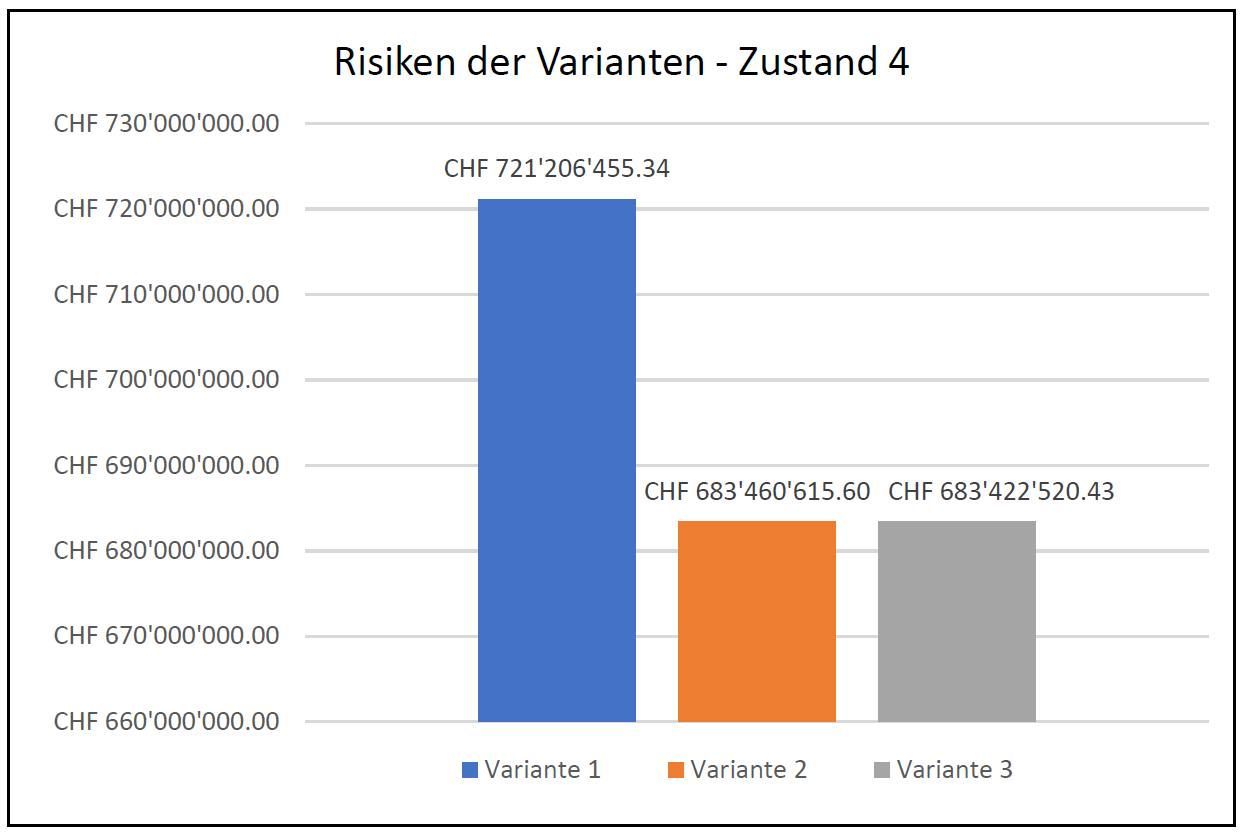
\includegraphics[width=.45\textwidth]{./figures/f-05-05-RisikenVarianteZ4}}
  \hfill
  \subfloat[][]{\label{img:Z4-V2/V3)}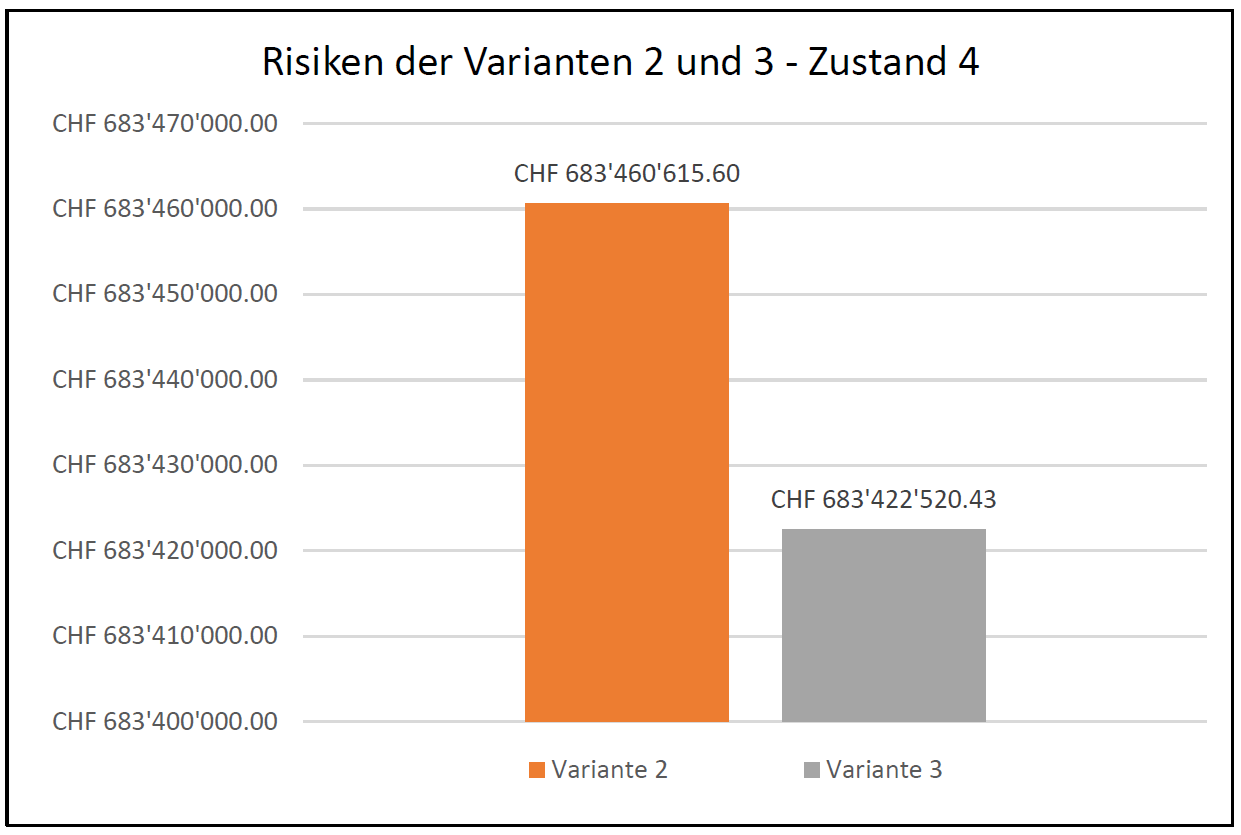
\includegraphics[width=.45\textwidth]{./figures/f-05-06-RisikenVariante-2und3-Z4}}
\caption[Verkehrsaufkommen]{Tägliches Verkehraufkommen Brunnenstrasse}
  \label{fig:Z4}
\end{figure}



% ===========================================================================
% EOF
%

%%% Local Variables:
%%% mode: latex
%%% TeX-master: "../main"
%%% End:


% Chapter 6
% ---------
%=============================================================================
% Thesis Template in LaTex
%
% File:  06-Diskussion.tex -- Diskussion
% Author(s): Cyrano Golliez <golliezc@student.ethz.ch>
%
% Creation:  27 Jan 2014
% Time-stamp: <Tue 2013-08-13 20:14 juergen>
%
% Copyright (c) 2014 Infrastructure Management Group (IMG)
%               http://ibi.ethz.ch
%
% More information on LaTeX: http://www.latex-project.org/
%=============================================================================

\chapter{Diskussion}
\label{chap:Diskussion}

In diesem Kapitel wird die in Abschnitt \ref{chap:Resultate} als optimal erachtete Lösung untersucht. Einerseits werden die Zustände 1 bis 4 mit dem Grundzustand 0 verglichen und andererseits die einzelne Kostenstrukturen in den verschiedenen Zuständen untersucht. Dies geschieht, um die als optimal erachtete Variante auf ihre Belastbarkeit in einer allfälligen Diskussion zuprüfen.

\paragraph{Zustand 0}

Gemäss dem Risikovergleich in Abschnitt \ref{chap:Resultate} ist im Zustand 0 die bestmögliche Variante für die Zukunft von Uster die Variante 2.  
Bei näherer Betrachtung der in Abbildung \ref{img:KostenZ0} dargestellten Reisezeitkosten und Unterhaltskosten der Varianten wird verdeutlicht, dass die Kosten die in der Variante 1 aufgrund der verlängerten Wartezeit entstehen, die Mehrkosten infolge Bau und Wartung der Variante 2, bei einer Betrachtung der Gesamtkosten über einen Zeitraum von 40 Jahren, um ein vielfaches übersteigen. Die Mehrkosten die bei der Ausführung der Variante 2 infolge höherer Bau- und Wartungskosten enstehen, betragen 1'238'600 CHF wohingegen die Mehrkosten die infolge der Variante 1, aufgrund der höheren Reisezeitkosten entstehen 38'984'439 CHF betragen. 

Durch diesen Vergleich wird verdeutlicht, dass sich die Variante 1, welche die Option "nichts zu verändern" darstellt, über den betrachteten Zeitraum von 40 Jahren nicht lohnenen wird. Die Mehrkosten die den Nutzern des Bahnübergangs und somit auch indirekt der Stadt Uster infolge der verlängerten Wartezeit entstehen, übersteigen die geforderten Inverstitionskosten für den Bau der Velounterführung um ein vielfaches. Im Fall der Variante 3 trifft dies nicht zu, weshalb sich ein solches Inverstment unter den Annahmen des Grundzustandes nicht lohnt.

\begin{figure}[h!]
  \centering
  \subfloat[][]{\label{img:}\includegraphics[width=.45\textwidth]{./figures/06-01-Unterhaltskosten-Z0}}
  \hfill
  \subfloat[][]{\label{img:}\includegraphics[width=.45\textwidth]{./figures/06-02-Reisezeitkosten-Z0}}
\caption[Verkehrsaufkommen]{Tägliches Verkehraufkommen Brunnenstrasse}
  \label{img:KostenZ0}
\end{figure}

\begin{IMleftrightskip}
Die Kosten wurden analog der in Abschnitt \ref{subsec:BerechnungRisiken} erläuterten Risikoberechnung ermittelt. Dies gilt für alle weiteren erwähnten Kostenstrukturen.
\end{IMleftrightskip}

Demnach lohnt sich der Bau der Variante 2 für die Stadt Uster bei einer Betrachtung der Gesamtkosten über 40 Jahre und das entstehende Risiko rechtfertigt die höheren Investitionskosten zu Beginn des untersuchten Zeitraum. 

\paragraph{Zustand 1}

Gemäss Abschnitt \ref{chap:Resultate} ist auch in Zustand 1 die Variante 2 die optimale Lösung. Somit hat die Veränderung des E-Auto Anteiles keinen Einfluss auf die Wahl der optimalen Variante. \\
Infolge des Vergleichs der Zustände 0 und 1 ist ersichtlich, dass das Risiko der Variante 1 um 0.023\%, das Risiko der Varianten 2 um 0.024\% und das Risiko der Variante 3 um 0.017\% gegenüber dem jeweiligen Risiko im Zustand 0 ansteigt. Diese Abweichungen wäre, um den Effekt der die Veränderung des E-Auto Anteiles auf optimale Lösung hat, im Rahmen einer Hauptstudie zu untersuchen.

Bei der näheren Betrachtung der Umweltkosten wird ersichtlich, dass die Umweltkosten für alle 3 Varianten jeweils um einen Betrag von 163'555 CHF ansteigen. 
Ein konservative Prognose des E-Auto Anteil hat somit keinen Einfluss auf die Wahl der optimalen Variante. Demnach müsste die Variante 2 auch in einer Zukunft in der der Verbrennungsmotor weiterhin eine massgebende Rolle spielen wird, die als optimal zu erachtetende Variante sein, um die Verkehrssituation am Bahnübergang nachhaltig zu verbessern.


\paragraph{Zustand 2} 

Wie im Abschnitt \ref{chap:Resultate} dargestellt, hat die Veränderung der Unfallwahrscheinlichkeit keinen Einfluss auf die Wahl der optimalen Variante. 
Bei näherer Betrachtung der Unfallkosten, sieht man, dass sich die Veränderung der Unfallwahrscheinlichkeit deutlich auf die anfallenden Unfallkosten auswirkt. 
Die Abbildung \ref{img:UnfallVer.Z0-2} zeigt den Unfallkostenvergleich der Zustände 0 und 2. Die Unfallkosten aller Varianten im Zustand 0 betragen 451'469 CHF. Im Zustand 2 betragen die Unfallkosten der Variante 2 547'384 CHF und die Unfallkosten der Variante 3 321'649 CHF. Für die Variante 2 entspricht das einer Veränderung von 21.25\% und für die Variante 3 einer Abnahme von 28.75\%. 

\begin{figure}[h!]
	\centering
	\includegraphics[width=.45\textwidth]{figures/06-03-Unfallkostenvergleich-Z0-Z2}
	\caption[Unfallkostenvergleich: Zustand 0 und 2]{Unfallkostenvergleich: Zustand 0 und 2}
	\label{img:UnfallVer.Z0-2}
\end{figure}

Betrachtet nun hingegen die Veränderung der Risiken der Variante von Zustand 0 zu Zustand 2, so beträgt die Veränderung für die Variante 1 +0.01\% und für die Variante 3 -0.01\%. 
Somit ist die Variante 2 auch mit erhöhter Unfallgefahr die optimale Variante für die zukünftige Situation am Bahnübergang Brunnenstrasse. 
 

\paragraph{Zustand 3} 

Die Veränderung der Eintrittswahrscheinlichkeit, wie in Abschnitt \ref{subsec:Sensitivitätsanalyse} dargestellt, hat keinen Einfluss auf die Wahl der optimalen Variante. Jedoch ist die folgende Darstellung \ref{img:SzeVer-Z0} der Risiken der einzelnen Szenarien, insofern interessant, dass es den Effekt verdeutlicht der die Wahl der Eintrittswahrscheinlichkeit auf die Verteilung der Risiken hat. So kann mit der Gewichtung der möglichen zukünftigen Ereignisse, sprich den Prognosen der möglichen Zukunft, die berechneten Risiken beeinflusst werden. 

\begin{figure}[h!]
	\centering
	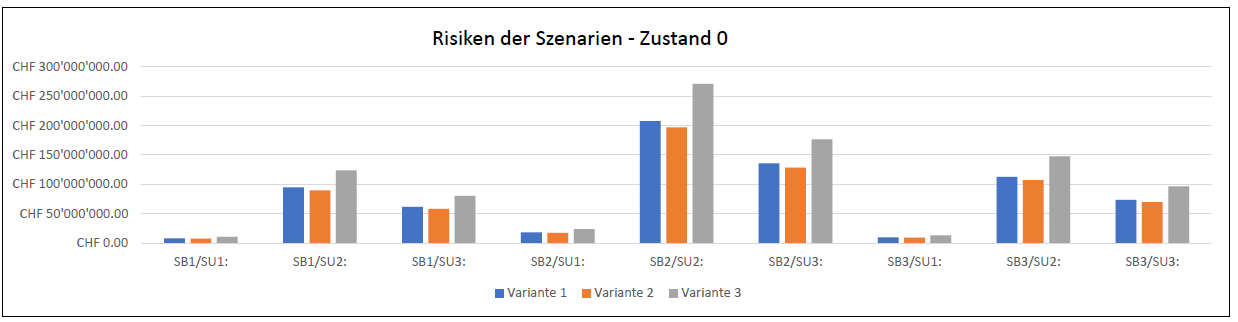
\includegraphics[width=.45\textwidth]{figures/f-06-04-RisikenSzenarienZ0}
	\caption[Szenarienvergleich im Zustand 0]{Vergleich der Risiken der Szenarien im Zustand 0}
	\label{img:SzeVer-Z0}
\end{figure} 

Im Zustand 3 wird der Schwerpunkt der Gewichtung der Szenarien so gelegt, dass diejenigen Szenarien mehr gewicht erhalten, welche die höchsten Wachstumsprognosen voraussagen und demnach das grösste Verkehrsaufkommen simulieren. Der Effekt einer solchen Verschiebung auf die Szenarien wird in der nachfolgenden Abbildung \ref{img:SzeVer-Z3} verdeutlicht. 

\begin{figure}[h!]
	\centering
	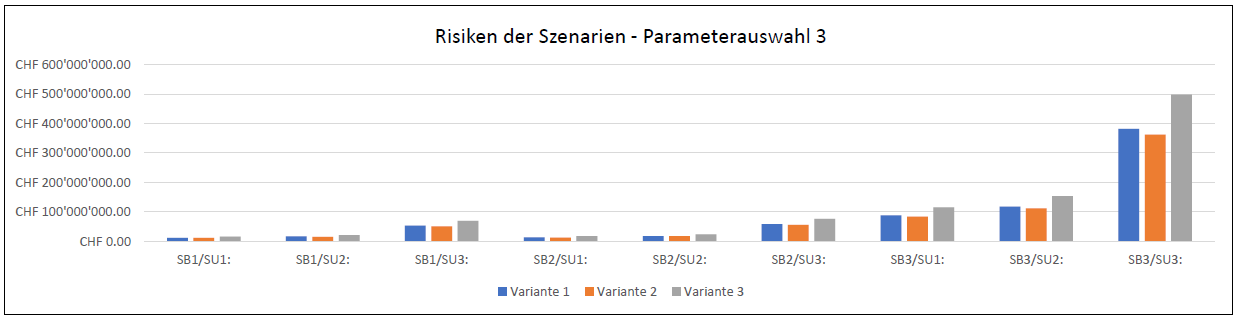
\includegraphics[width=.45\textwidth]{figures/f-06-05-RisikenSzenarienZ3}
	\caption[Szenarienvergleich im Zustand 3]{Vergleich der Risiken der Szenarien im Zustand 3}
	\label{img:SzeVer-Z3}
\end{figure} 

Auf die Wahl der optimalen Variante hat diese Veränderung keinen Einfluss, da die Risiken der Varianten jeweils um 5.5\% im Vergleich zum Zustand 0 steigen. Erst bei der Betrachtung der Nachkommastellen, lässt sich eine gewisse Unterscheidung feststellen. So beträgt die Veränderung des Risiko der Variante 1 vom Zustand 0 zum Zustand 3 5.530\%, die Veränderung des Risiko der Variante 2 beträgt 5.518\% und die Veränderung des Risikos der Variante 3 5.525\%. Aus diesen geringfügigen Abweichung einen Rückschluss auf die im Rahmen des Zustand 3 veränderten Eigenschaften der Risikoberechnung zu machen, war im Rahmen dieser Projektarbeit nicht möglich und wäre im Rahmen einer Hauptstudie weiter zu untersuchen.


\paragraph{Zustand 4} 

in die anderere Richtung die Argumentation gegen die V2 -> fals für alle 3 die wartezeit steigt, weil noch mehr züge kommen, so dass amepelsystem nicht zu extra wartzeit führt, dann aber nur dann wäre die Variante 3 der Variante 2 überlegen... um wie viel...

%Die Kapazität für den ÖV ist in keiner Variante beeinträchtigt. Einen Ausbau der Kapazität ist nicht geplannt. Neubauten oder umstrukturierungen verschiedener Bushaltestellen ist im Rahmen der genaueren Bauausführung zu prüfen. \\

%Hier werden die Resultate diskutiert. 

%Der geplanten Stadterschliessungen West und Süd-Ost sind für die Förderung des Langsamverkehrs in der Stadt Uster von zentraler Bedeutung. So kann eine Entlastung des Zentrums und der Nord-Süd Achse entlang der Bahnhofstrasse nur realisiert werden wenn der MIV entlang der Westumfahrung um das Stadtzentrum herum geführt wird. 

%Dies ermöglicht gemäss STEK eine komfortable, durchgehende und direkte Verindung mit allenfals zu prüfender Vortrittsberechtigung. Die Infrastruktur dieser Radwege sollte ausschliesslich für diese Art von Verkehr zugelassen sein und gemäss STEK Kap.7 Tab. 1 mind. 4.8m breit sein. Um eine kreuzungsfreie Durchfahrt zu gewährleisten ist eine Ausführung in Anlehnung an den Aufbau einer Autobahn zu prüfen.  

% ===========================================================================
% EOF
%

%%% Local Variables:
%%% mode: latex
%%% TeX-master: "../main"
%%% End:


% Chapter 7
% ---------
%=============================================================================
% Thesis Template in LaTex
%
% File:  07-Schlussfolgerung.tex -- Schlussfolgerung und Ausblick
% Author(s): Cyrano Golliez <golliezc@student.ethz.ch>
%
% Creation:  27 Jan 2014
% Time-stamp: <Tue 2013-08-13 20:14 juergen>
%
% Copyright (c) 2014 Infrastructure Management Group (IMG)
%               http://ibi.ethz.ch
%
% More information on LaTeX: http://www.latex-project.org/
%=============================================================================

\chapter{Schlussfolgerung und Ausblick}
\label{chap:Schlussfolgerung}


Hier wird die Schlussfolgerung aus der Diskussion der Resultate gezogen. 

Somit kann die geplante Veloroute eine Reduktion der Belastung der Öffentliche Hand, in Form der Reduktion der Schadstoffemission, erreichen. 	
Die Schwierigkeit diese Kosten zu modelieren liegt in der nicht direkt messbaren Beziehung zwischen Schadstoffbelastung und daraus resultierenden Kosten. Jedoch ist zu vermerken das die Emissionen direkt von der Anzahl an motorisierten Fahrzeuge abhängt die auf der Infrastruktur verkehren.

% ===========================================================================
% EOF
%

%%% Local Variables:
%%% mode: latex
%%% TeX-master: "../main"
%%% End:



%___________________________________


% Reference
% ---------
% Style for Germen text
%\bibliographystyle{chicago-german}

% Style for Englisch text
%\bibliographystyle{chicago}

%\bibliography{literature}

\newpage
\printbibliography[heading=bibintoc, title=Literaturverzeichnis]



% Appendix
% --------
\appendix
\addchap{Anhang}
\label{chap:Anhang}
\refstepcounter{chapter}

\section{DTV Modellierung}
\label{subsec:DTVModellierung}

\begin{figure}[h!]
	\centering
	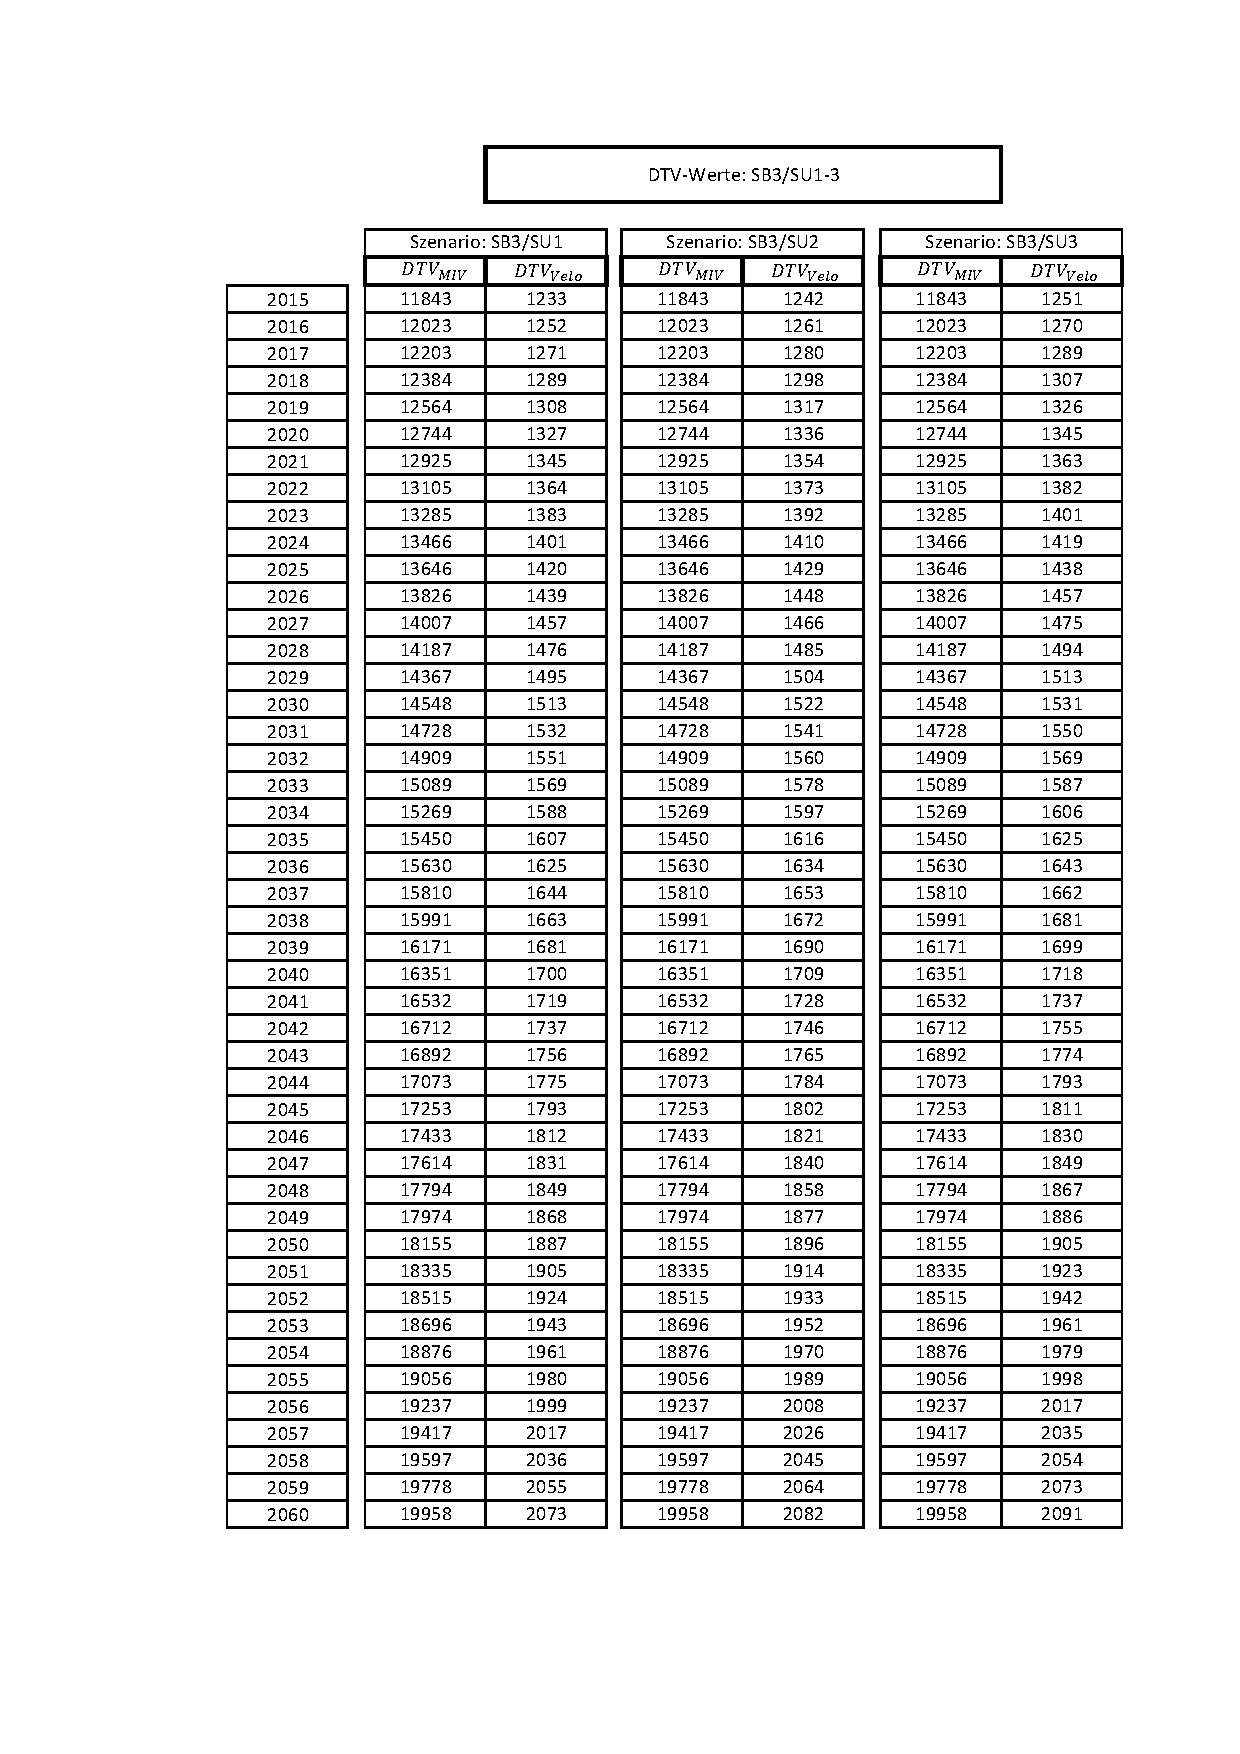
\includegraphics[width=\textwidth]{figures/f-00-10-01-DTV-Modellierung}
	\caption{Berechnung des DTV}
	\label{img:DTVModellierung}
\end{figure}


\section{Kostenberechung der Varianten}
\label{sec:Ahangkostenberechnug}

%=============================================================================
% Thesis Template in LaTex
%
% File:  Anhang.tex -- Anhang
% Author(s): Cyrano Golliez <golliezc@student.ethz.ch>
%
% Creation:  27 Jan 2014
% Time-stamp: <Tue 2013-08-13 20:14 juergen>
%
% Copyright (c) 2014 Infrastructure Management Group (IMG)
%               http://ibi.ethz.ch
%
% More information on LaTeX: http://www.latex-project.org/
%=============================================================================

%----Kostenberechnung der Varianten---------

\begin{figure}[h!]
	\centering
	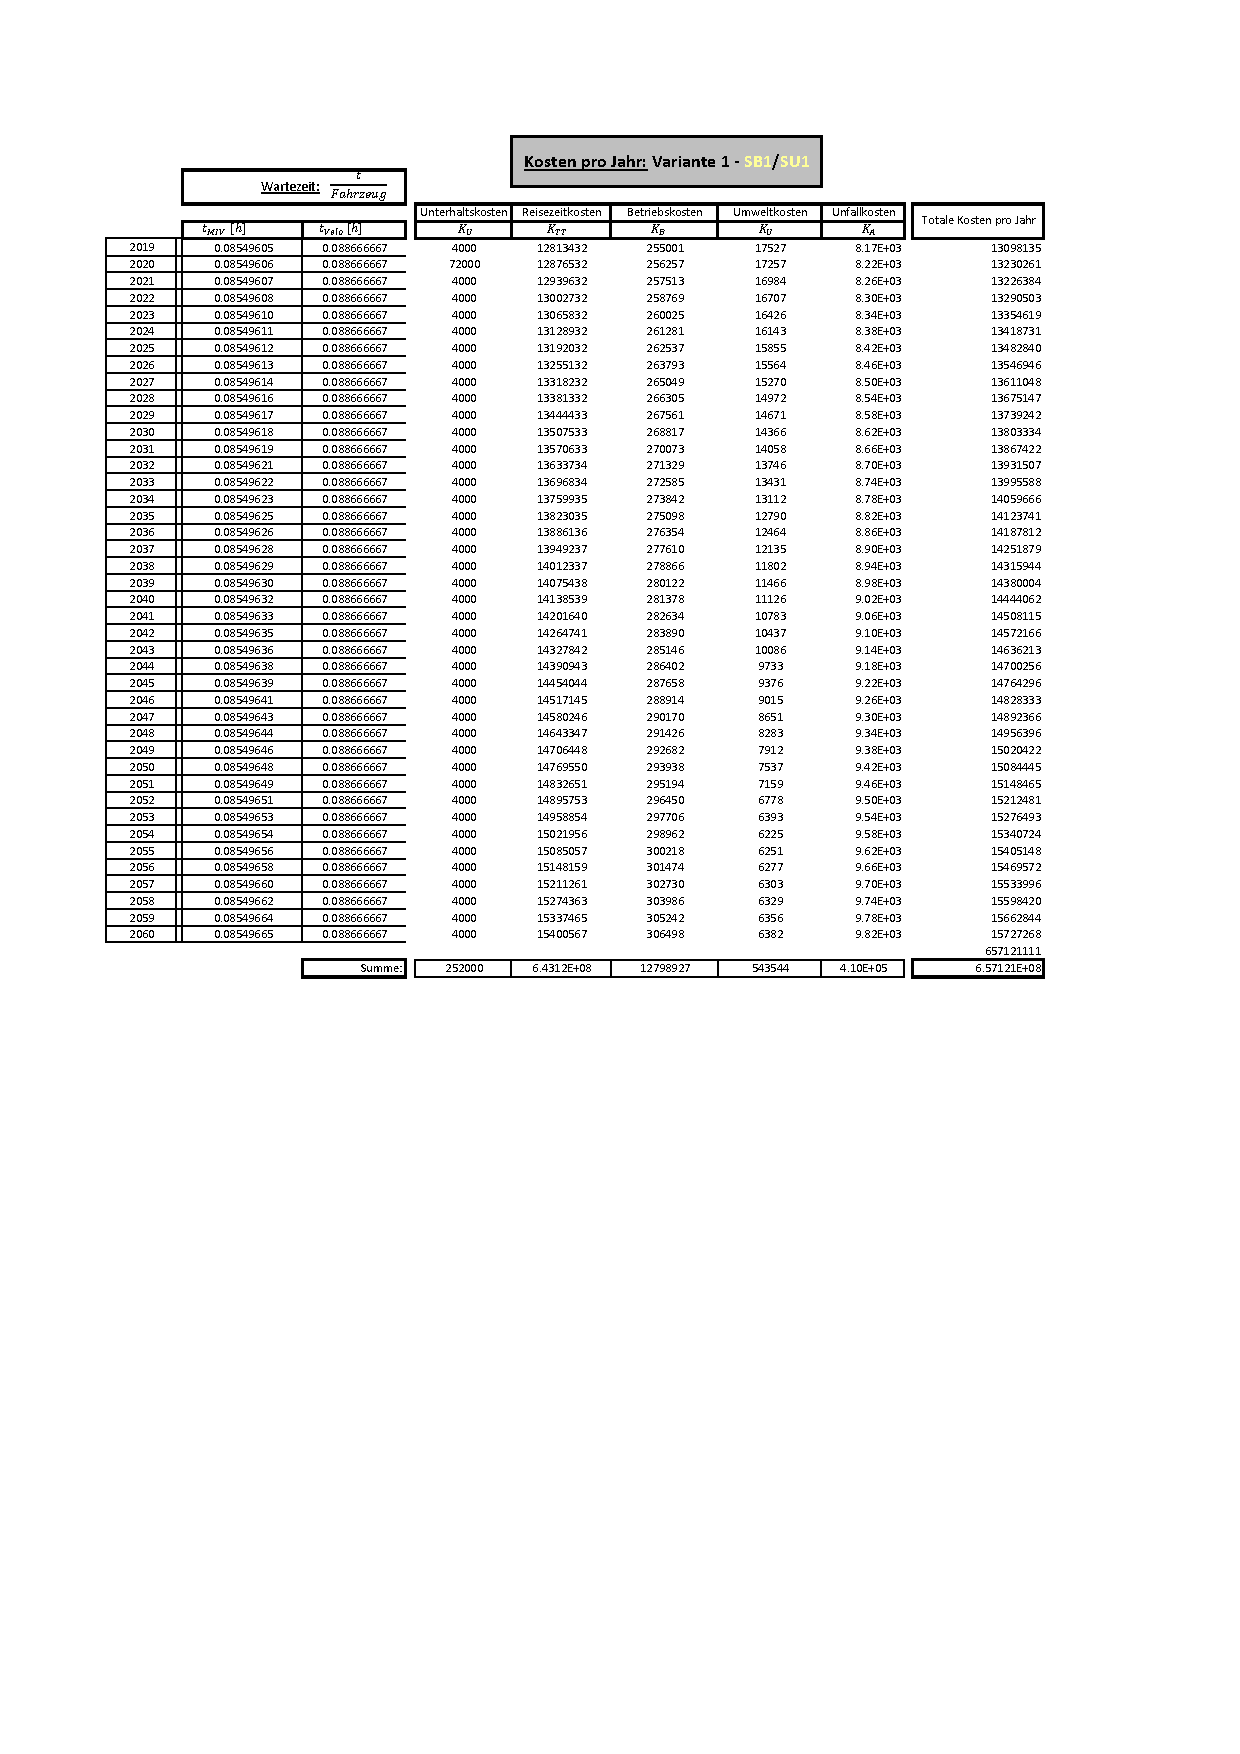
\includegraphics[width=\textwidth]{figures/Anhang/f-00-A-V1-B1-U1}
	\caption{Kostenberechung Variante 1 - SB1/SU1}
\end{figure}

\begin{figure}[h!]
	\centering
	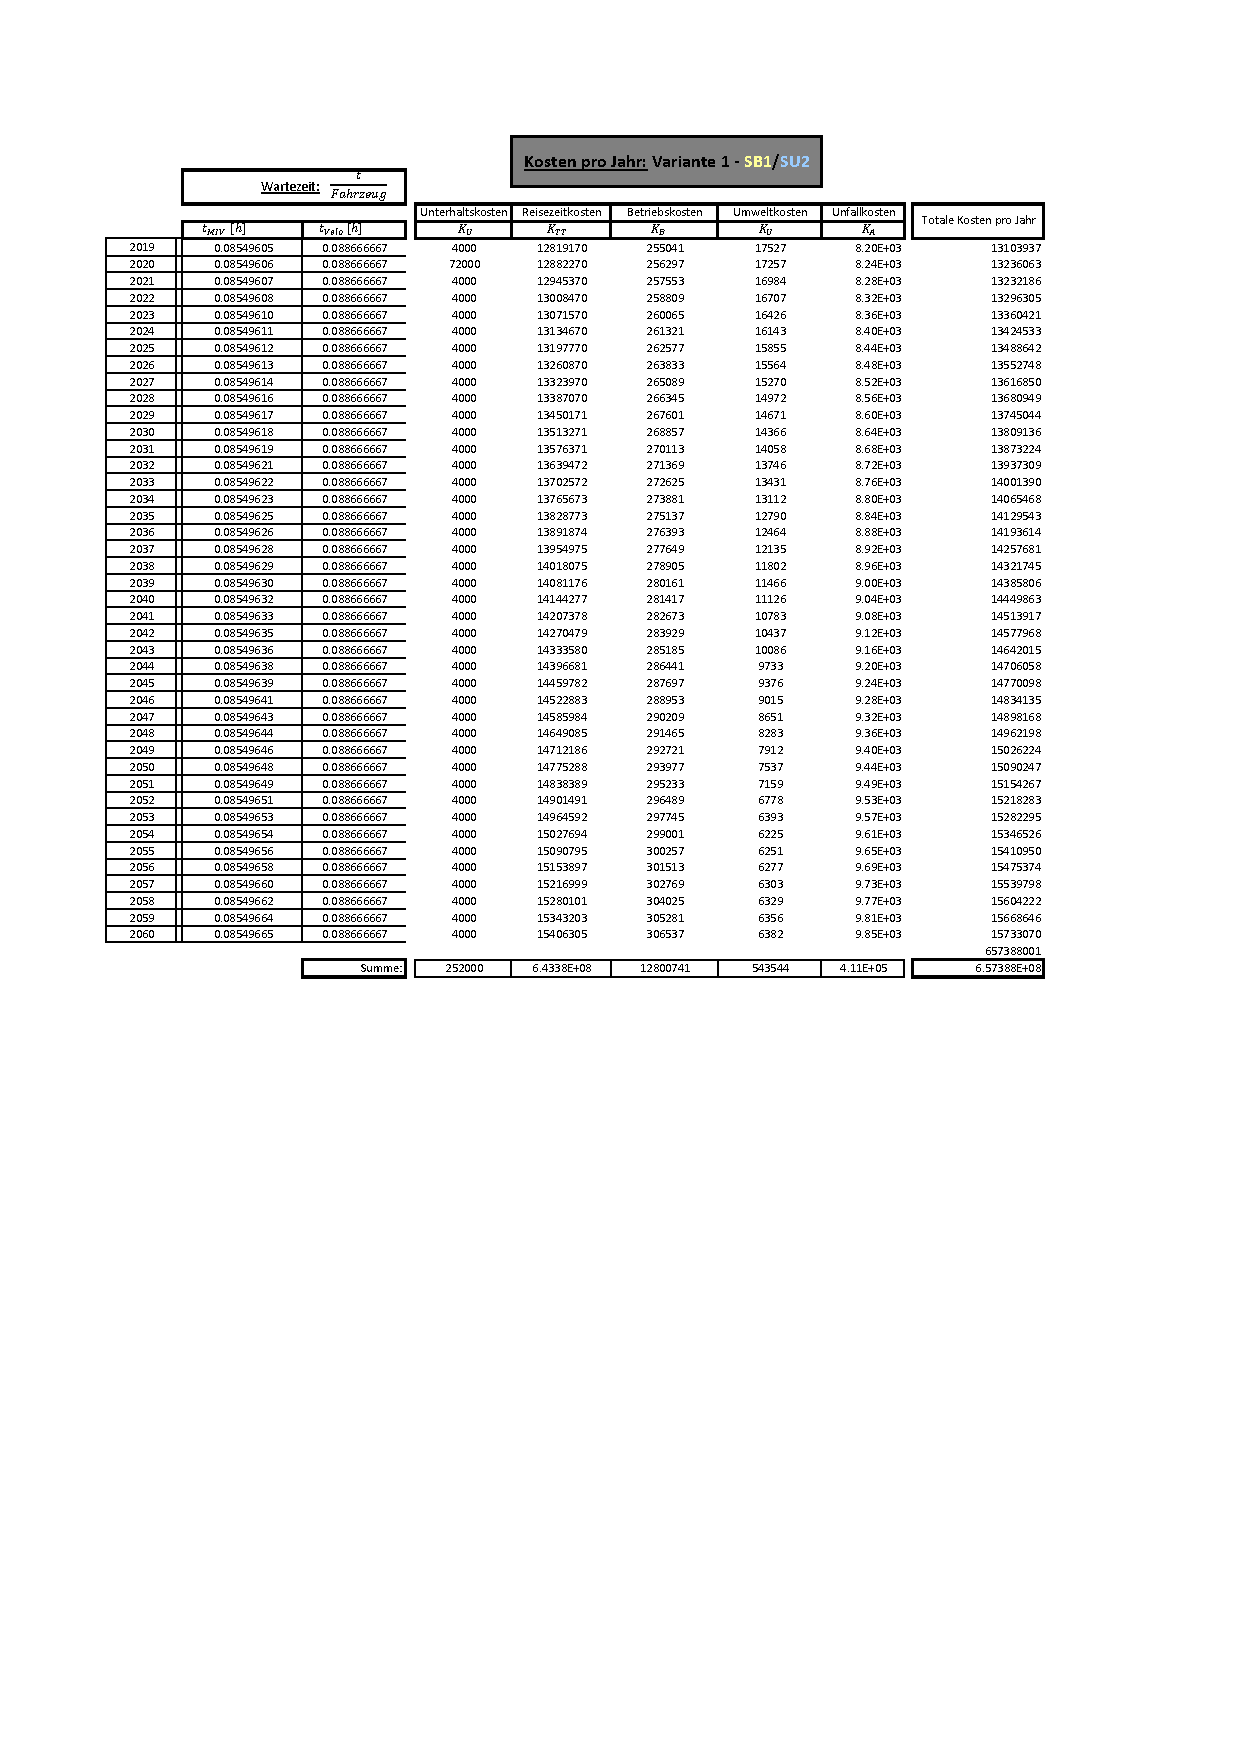
\includegraphics[width=\textwidth]{figures/Anhang/f-00-A-V1-B1-U2}
	\caption{Kostenberechung Variante 1 - SB1/SU2}
\end{figure}

\begin{figure}[h!]
	\centering
	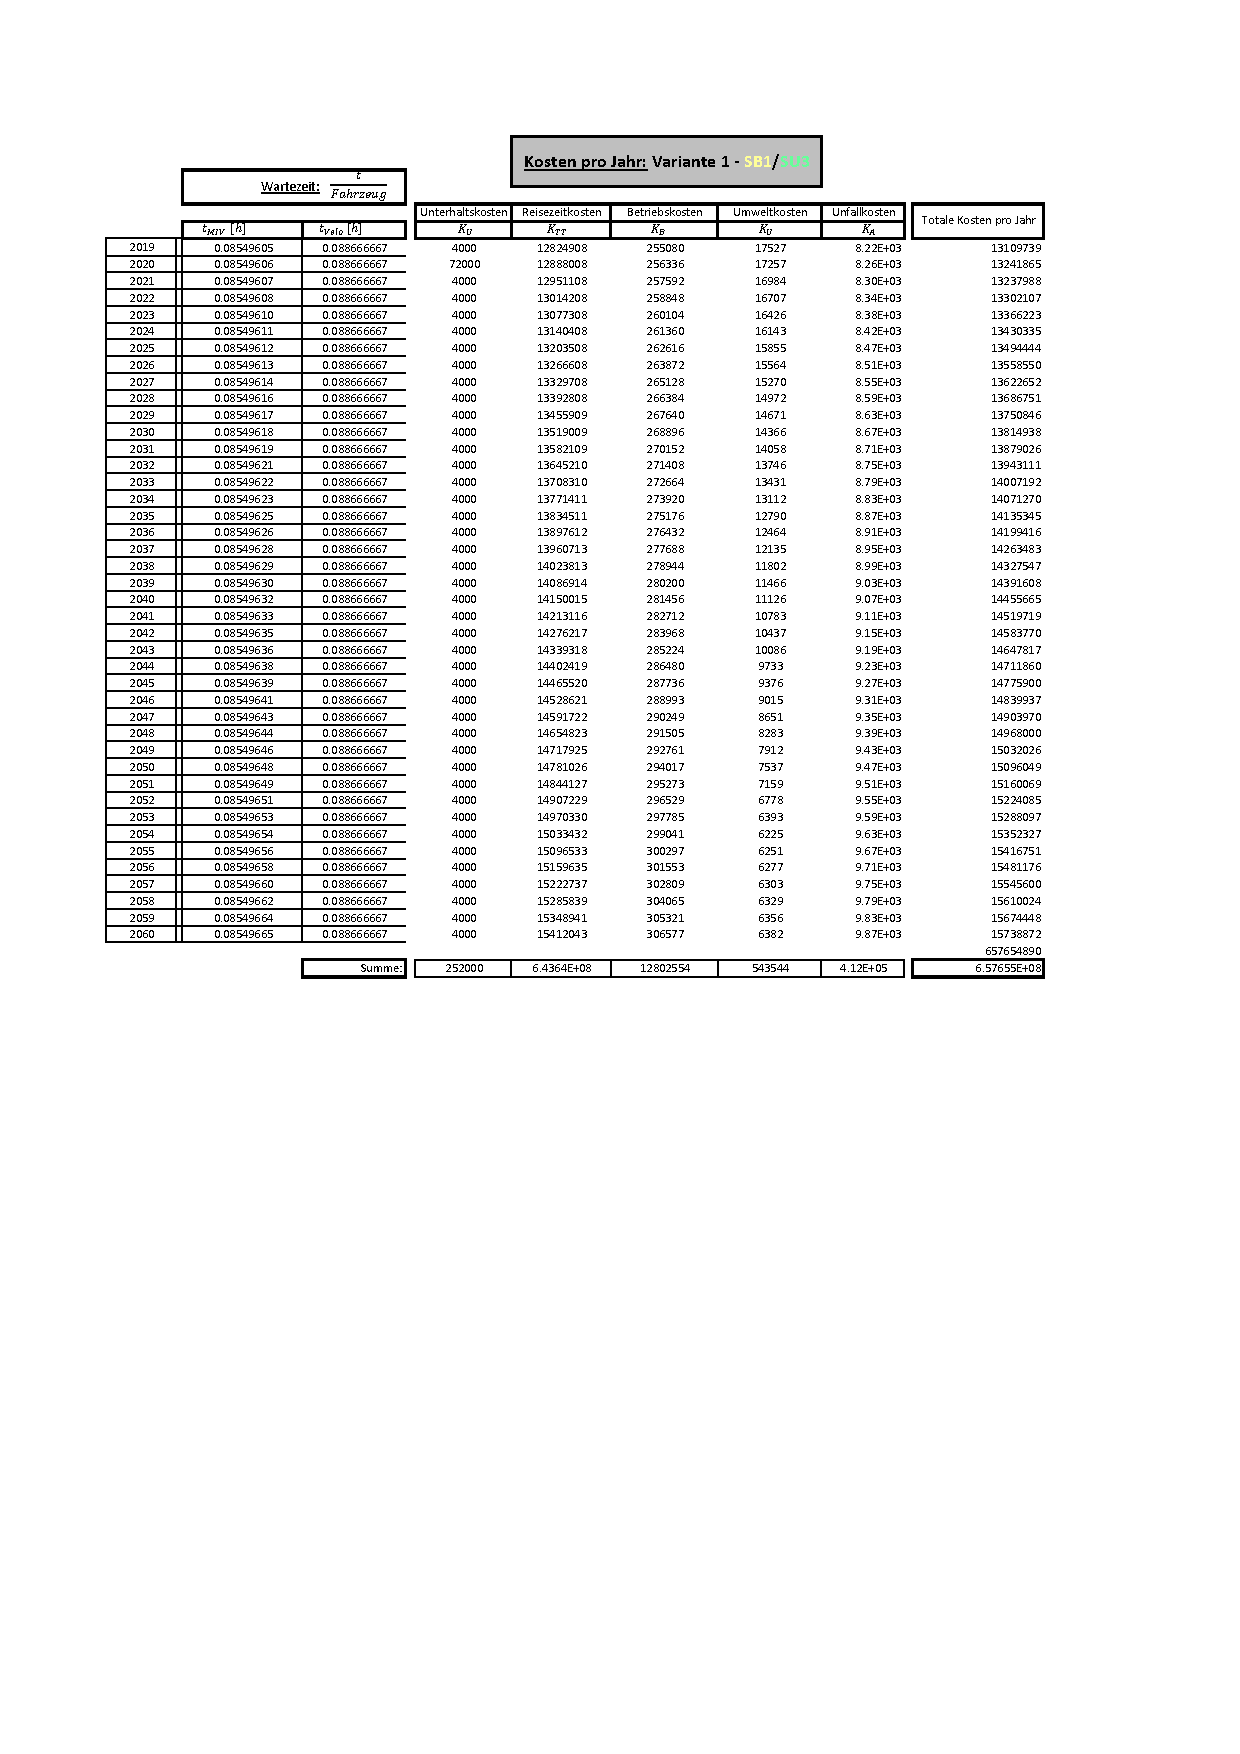
\includegraphics[width=\textwidth]{figures/Anhang/f-00-A-V1-B1-U3}
	\caption{Kostenberechung Variante 1 - SB1/SU3}
\end{figure}

\begin{figure}[h!]
	\centering
	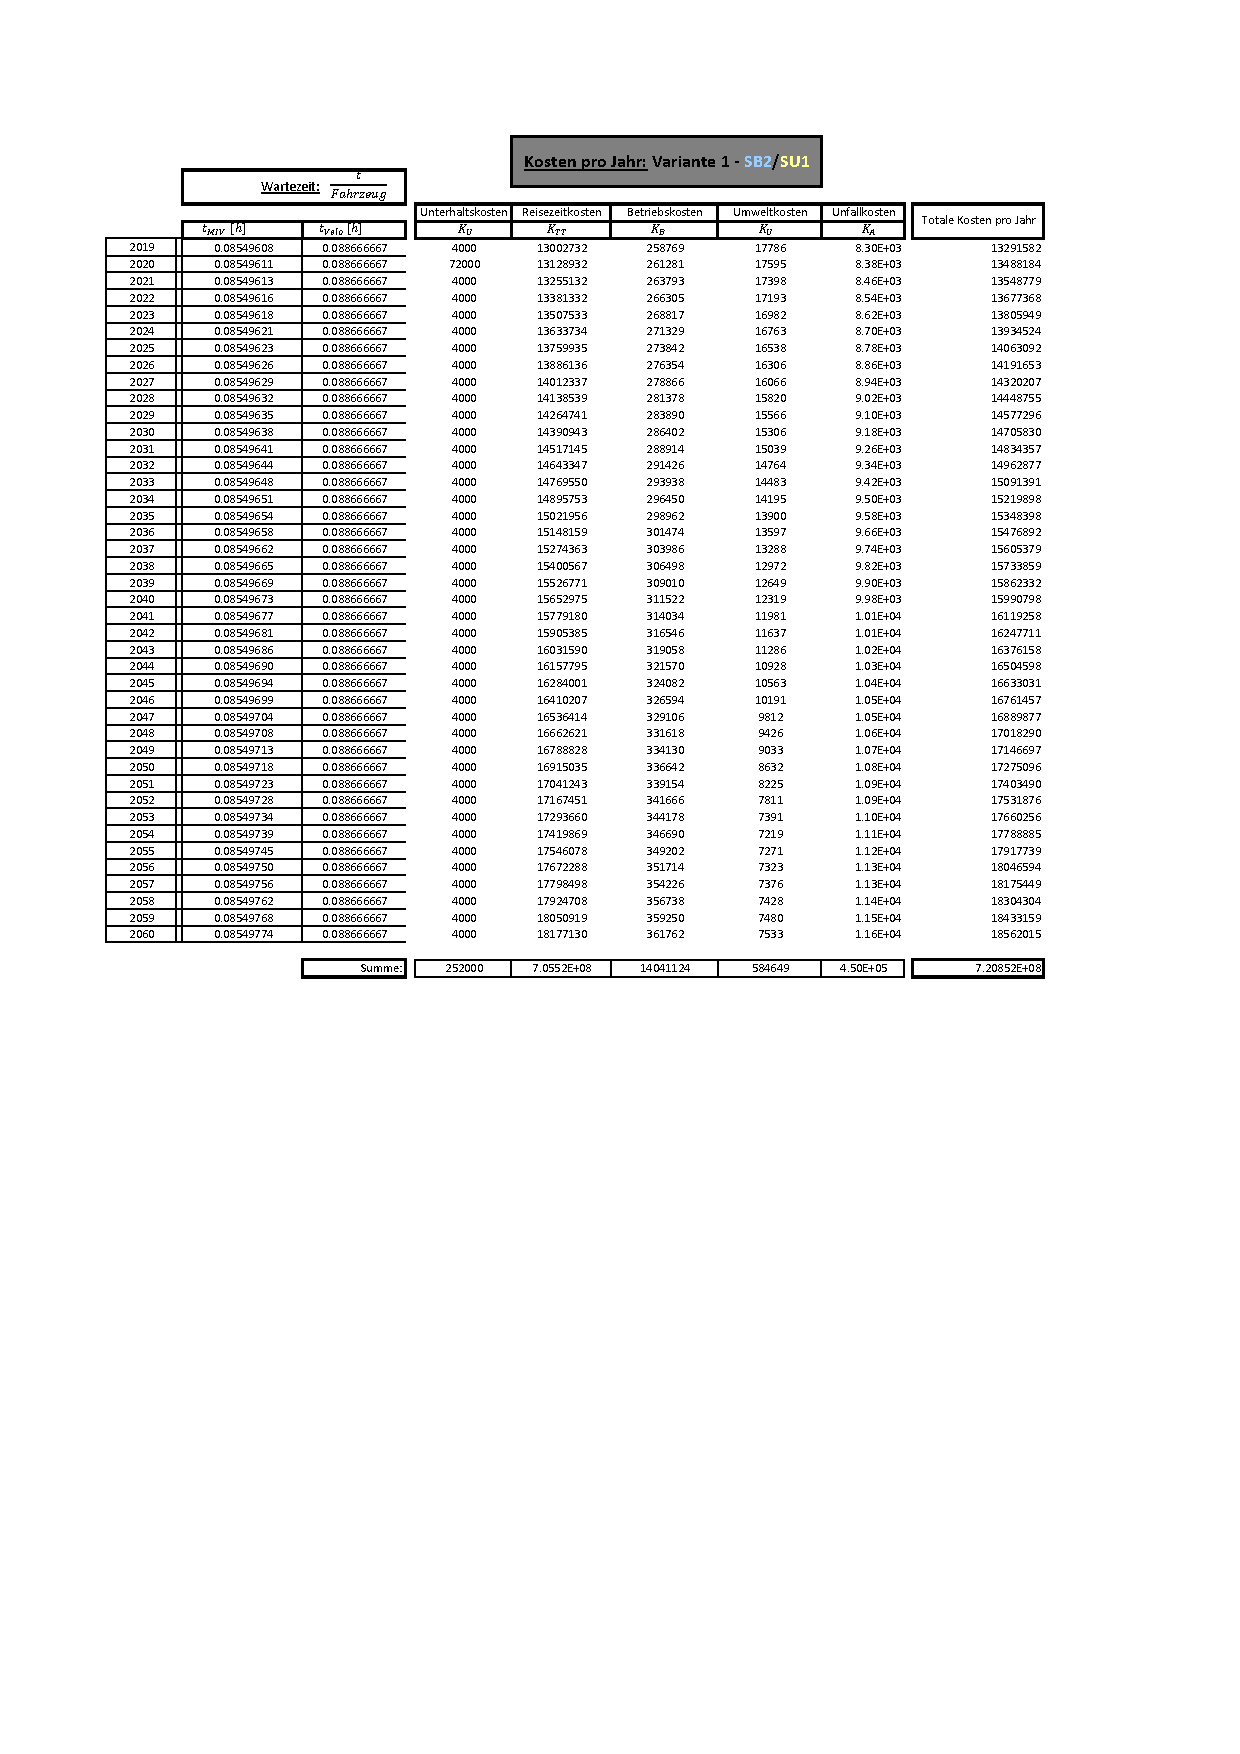
\includegraphics[width=\textwidth]{figures/Anhang/f-00-A-V1-B2-U1}
	\caption{Kostenberechung Variante 1 - SB2/SU1}
\end{figure}

\begin{figure}[h!]
	\centering
	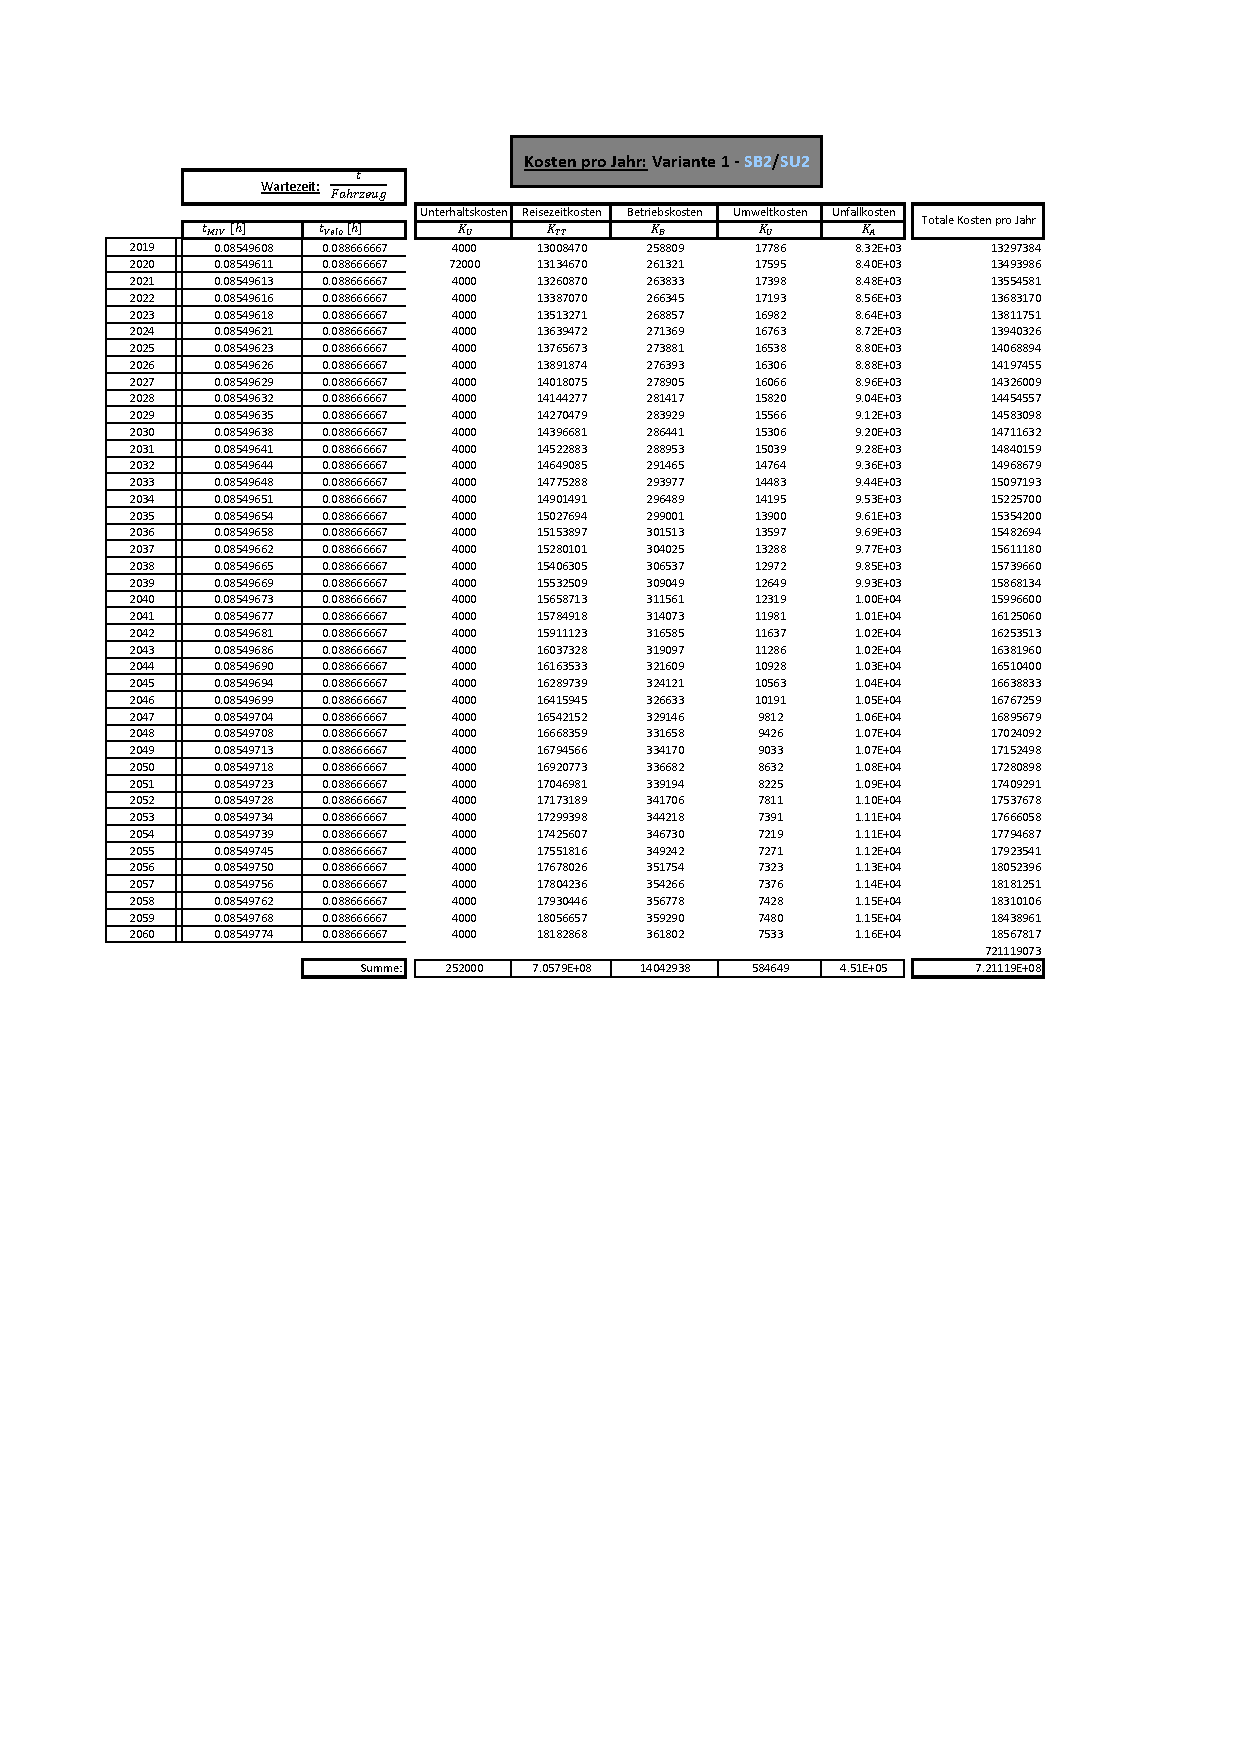
\includegraphics[width=\textwidth]{figures/Anhang/f-00-A-V1-B2-U2}
	\caption{Kostenberechung Variante 1 - SB2/SU2}
\end{figure}

\begin{figure}[h!]
	\centering
	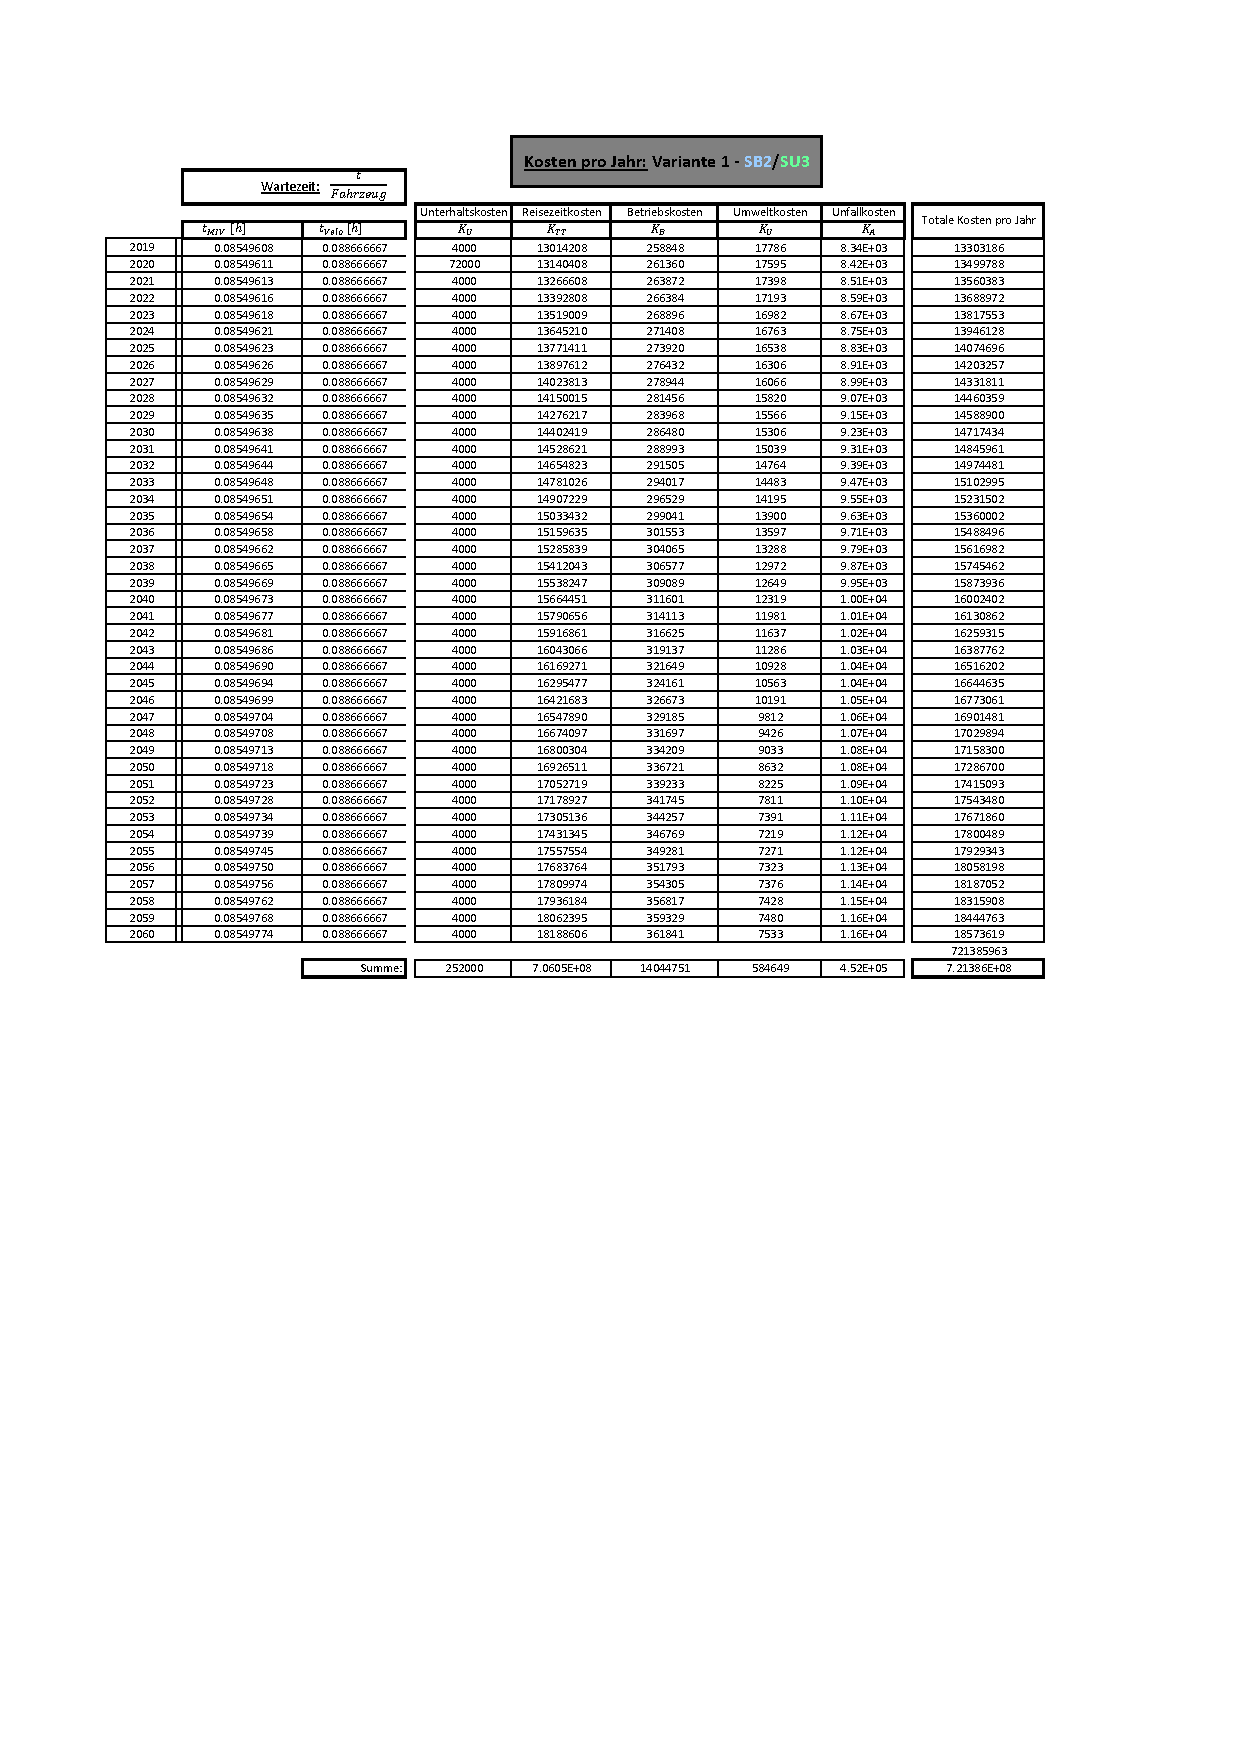
\includegraphics[width=\textwidth]{figures/Anhang/f-00-A-V1-B2-U3}
	\caption{Kostenberechung Variante 1 - SB2/SU3}
\end{figure}

\begin{figure}[h!]
	\centering
	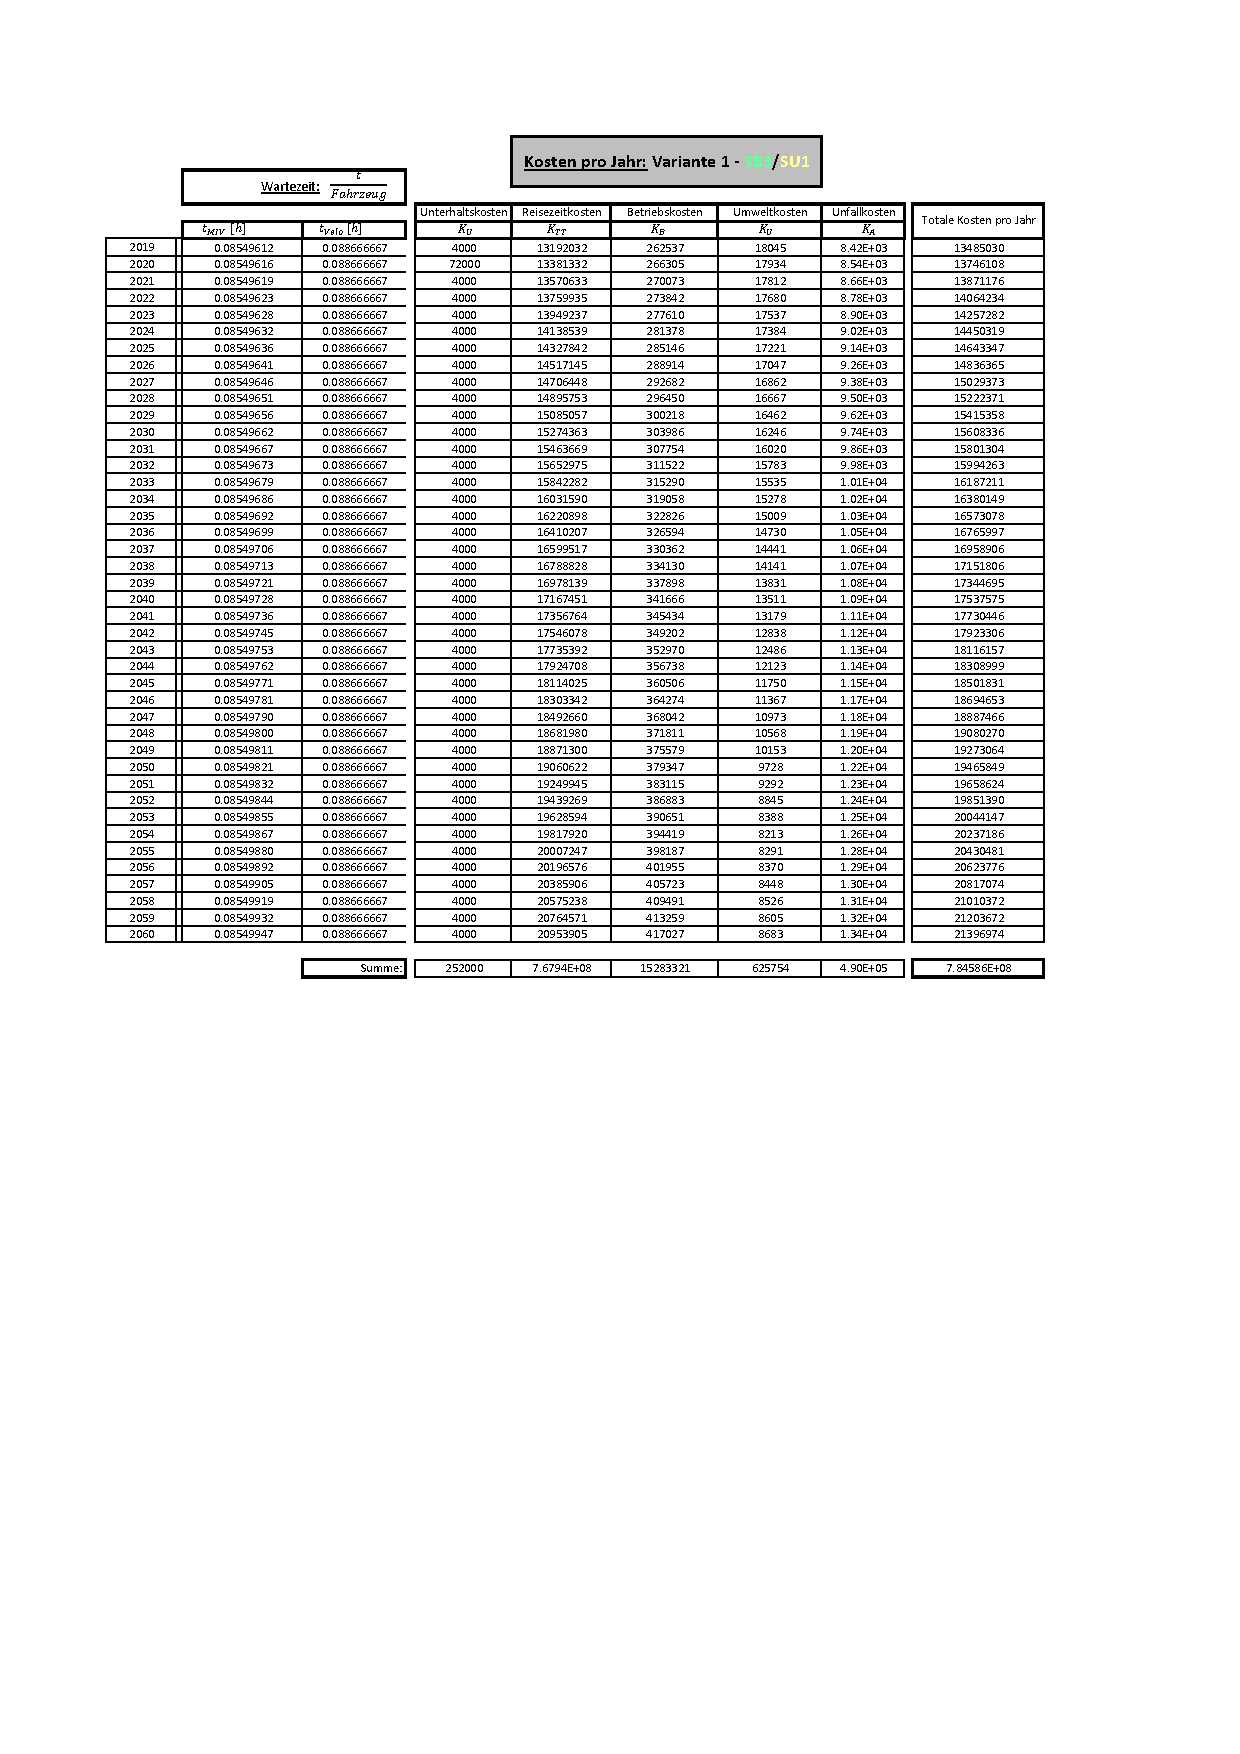
\includegraphics[width=\textwidth]{figures/Anhang/f-00-A-V1-B3-U1}
	\caption{Kostenberechung Variante 1 - SB3/SU1}
\end{figure}

\begin{figure}[h!]
	\centering
	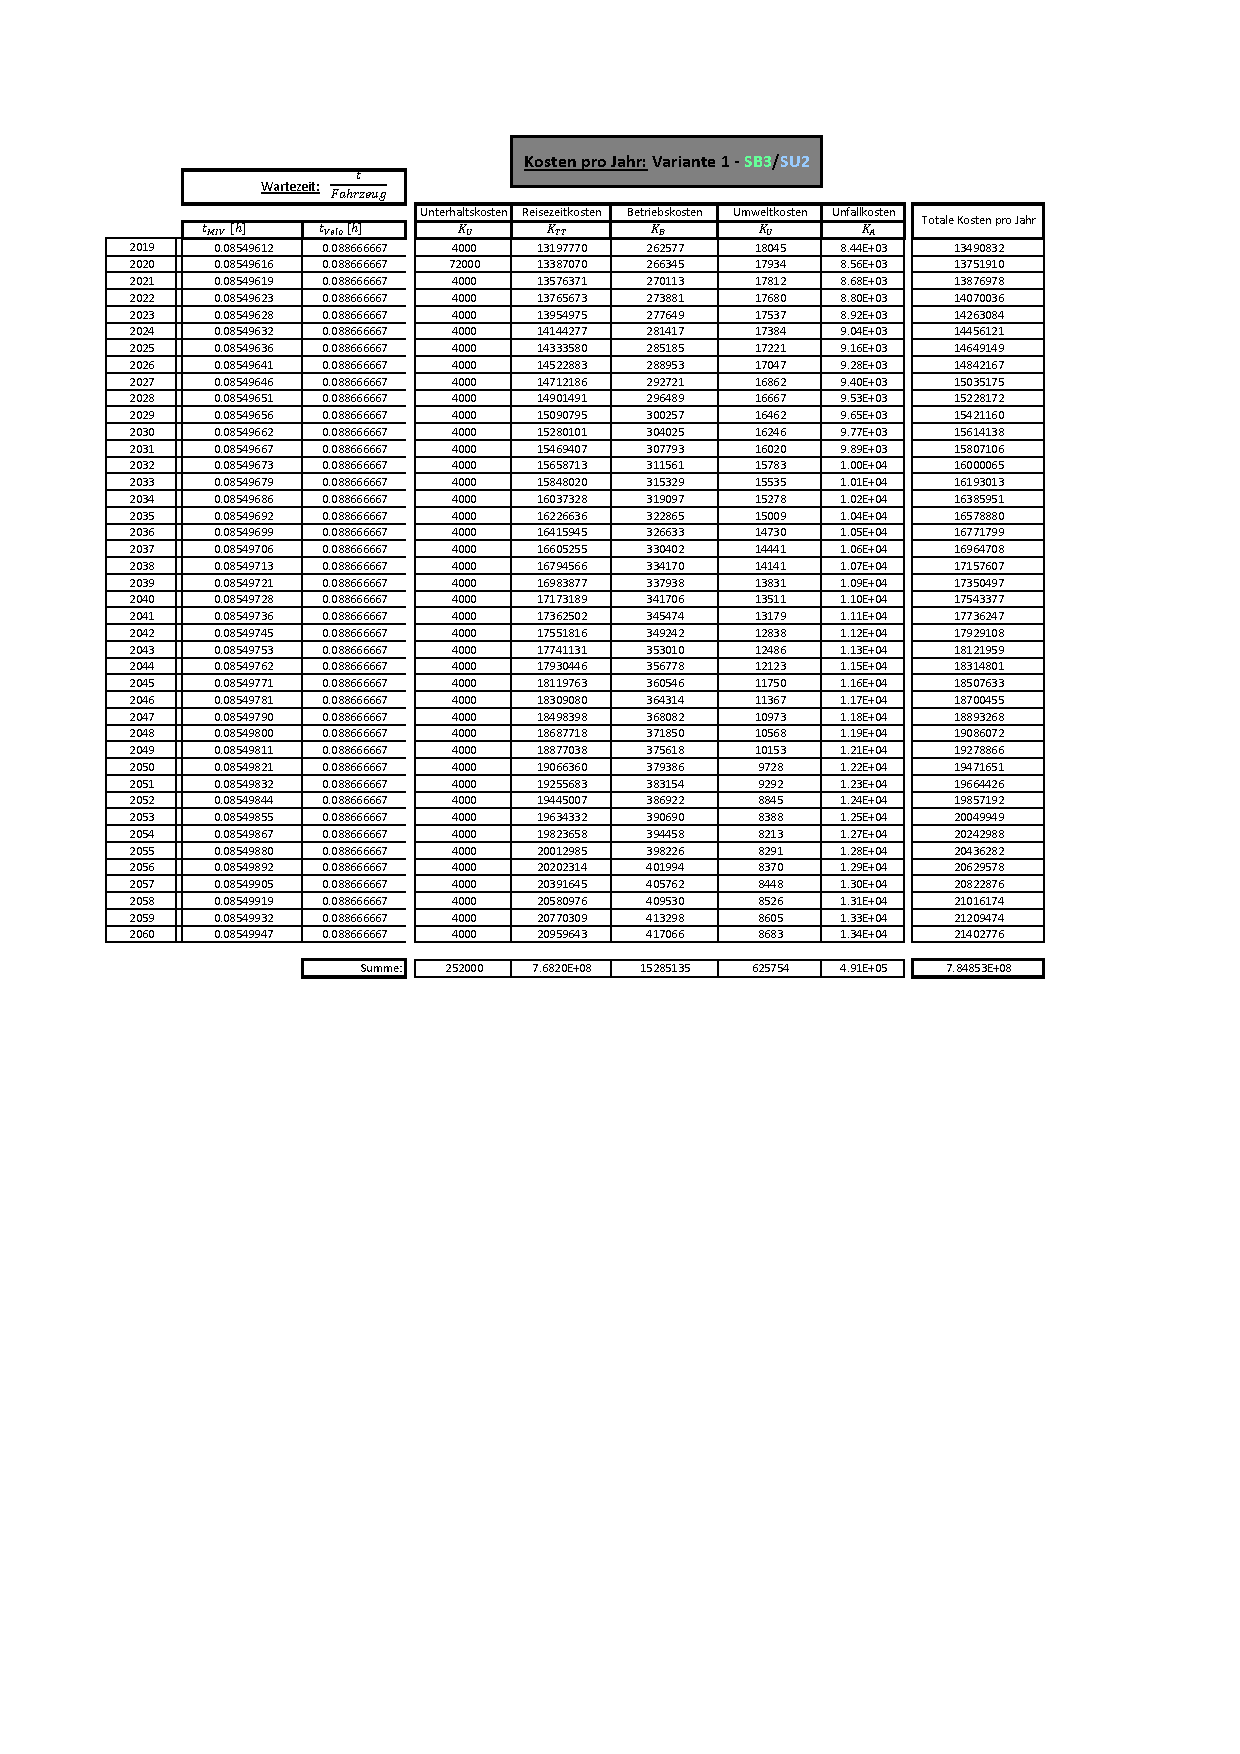
\includegraphics[width=\textwidth]{figures/Anhang/f-00-A-V1-B3-U2}
	\caption{Kostenberechung Variante 1 - SB3/SU2}
\end{figure}

\begin{figure}[h!]
	\centering
	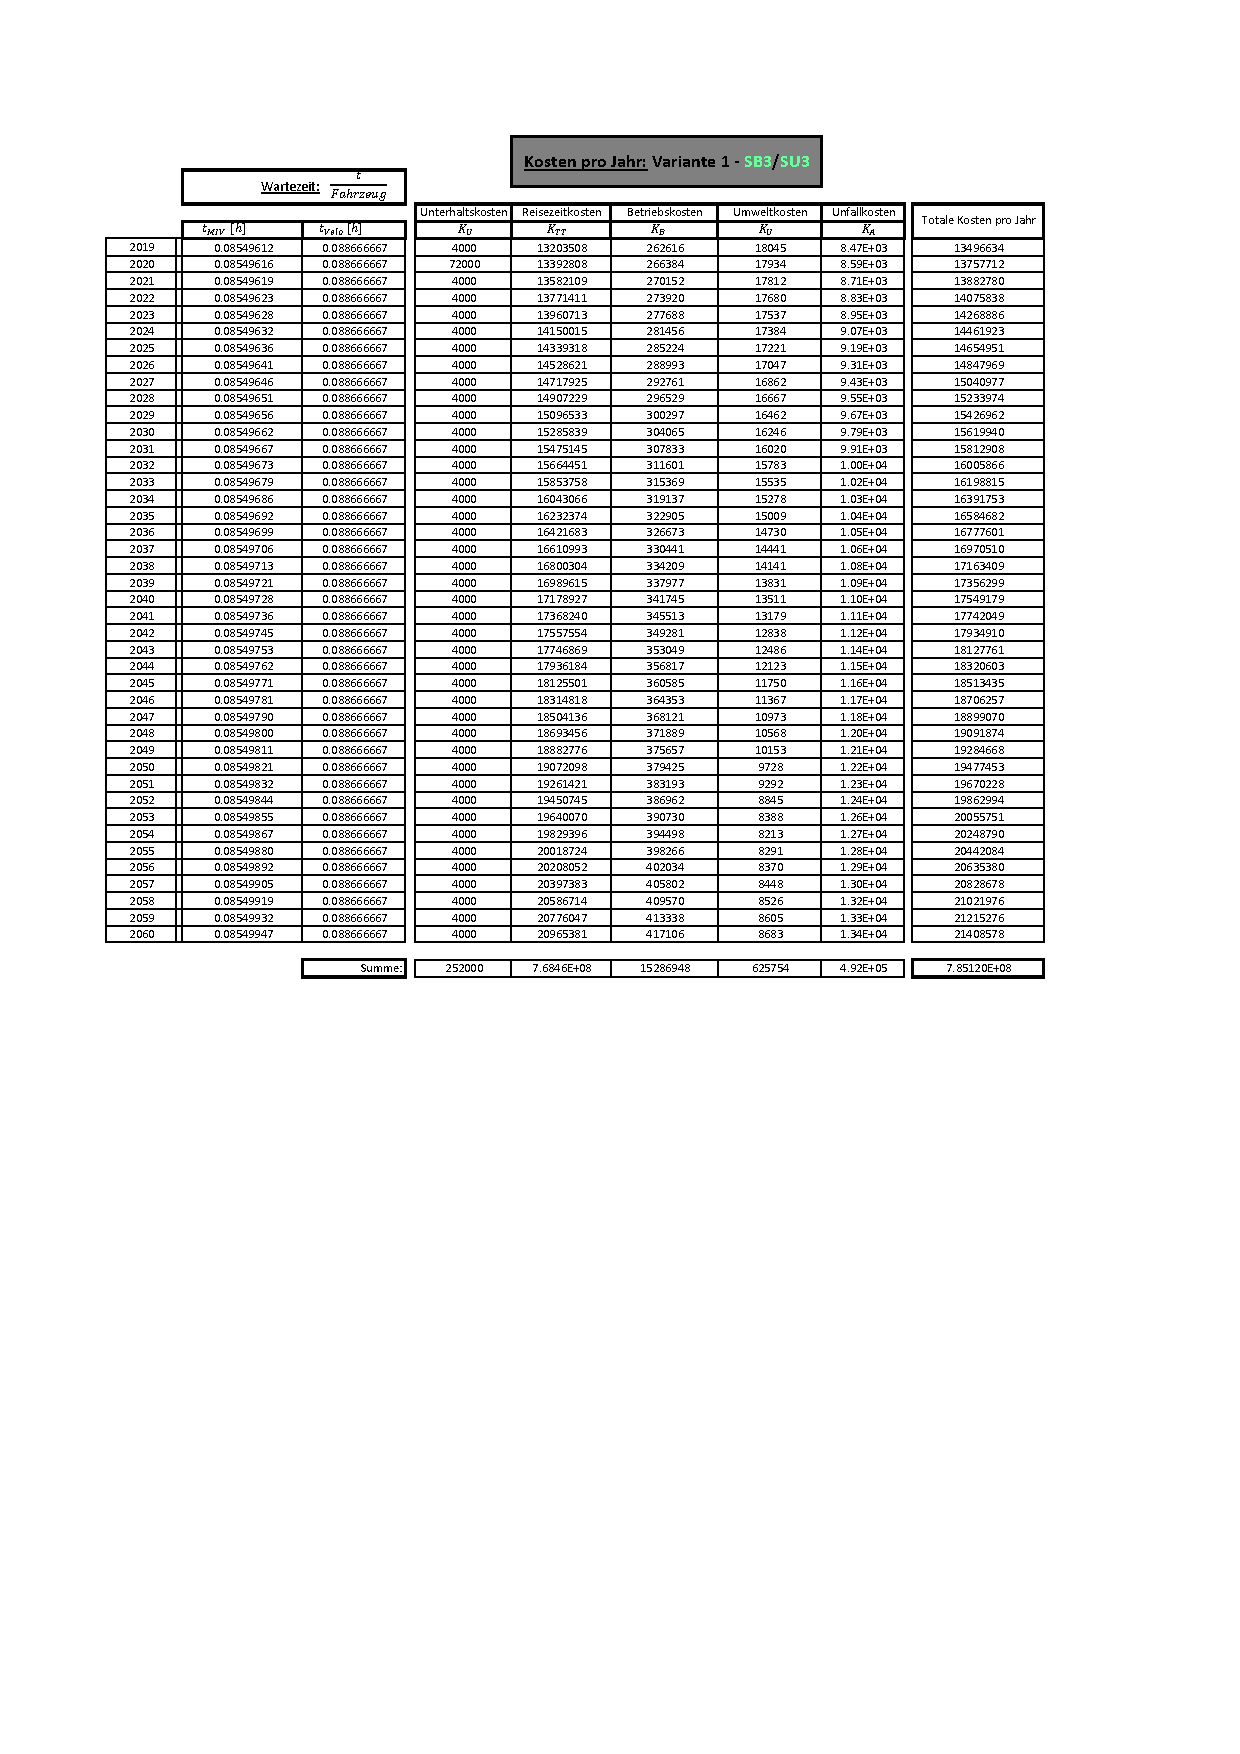
\includegraphics[width=\textwidth]{figures/Anhang/f-00-A-V1-B3-U3}
	\caption{Kostenberechung Variante 1 - SB3/SU3}
\end{figure}

\begin{figure}[h!]
	\centering
	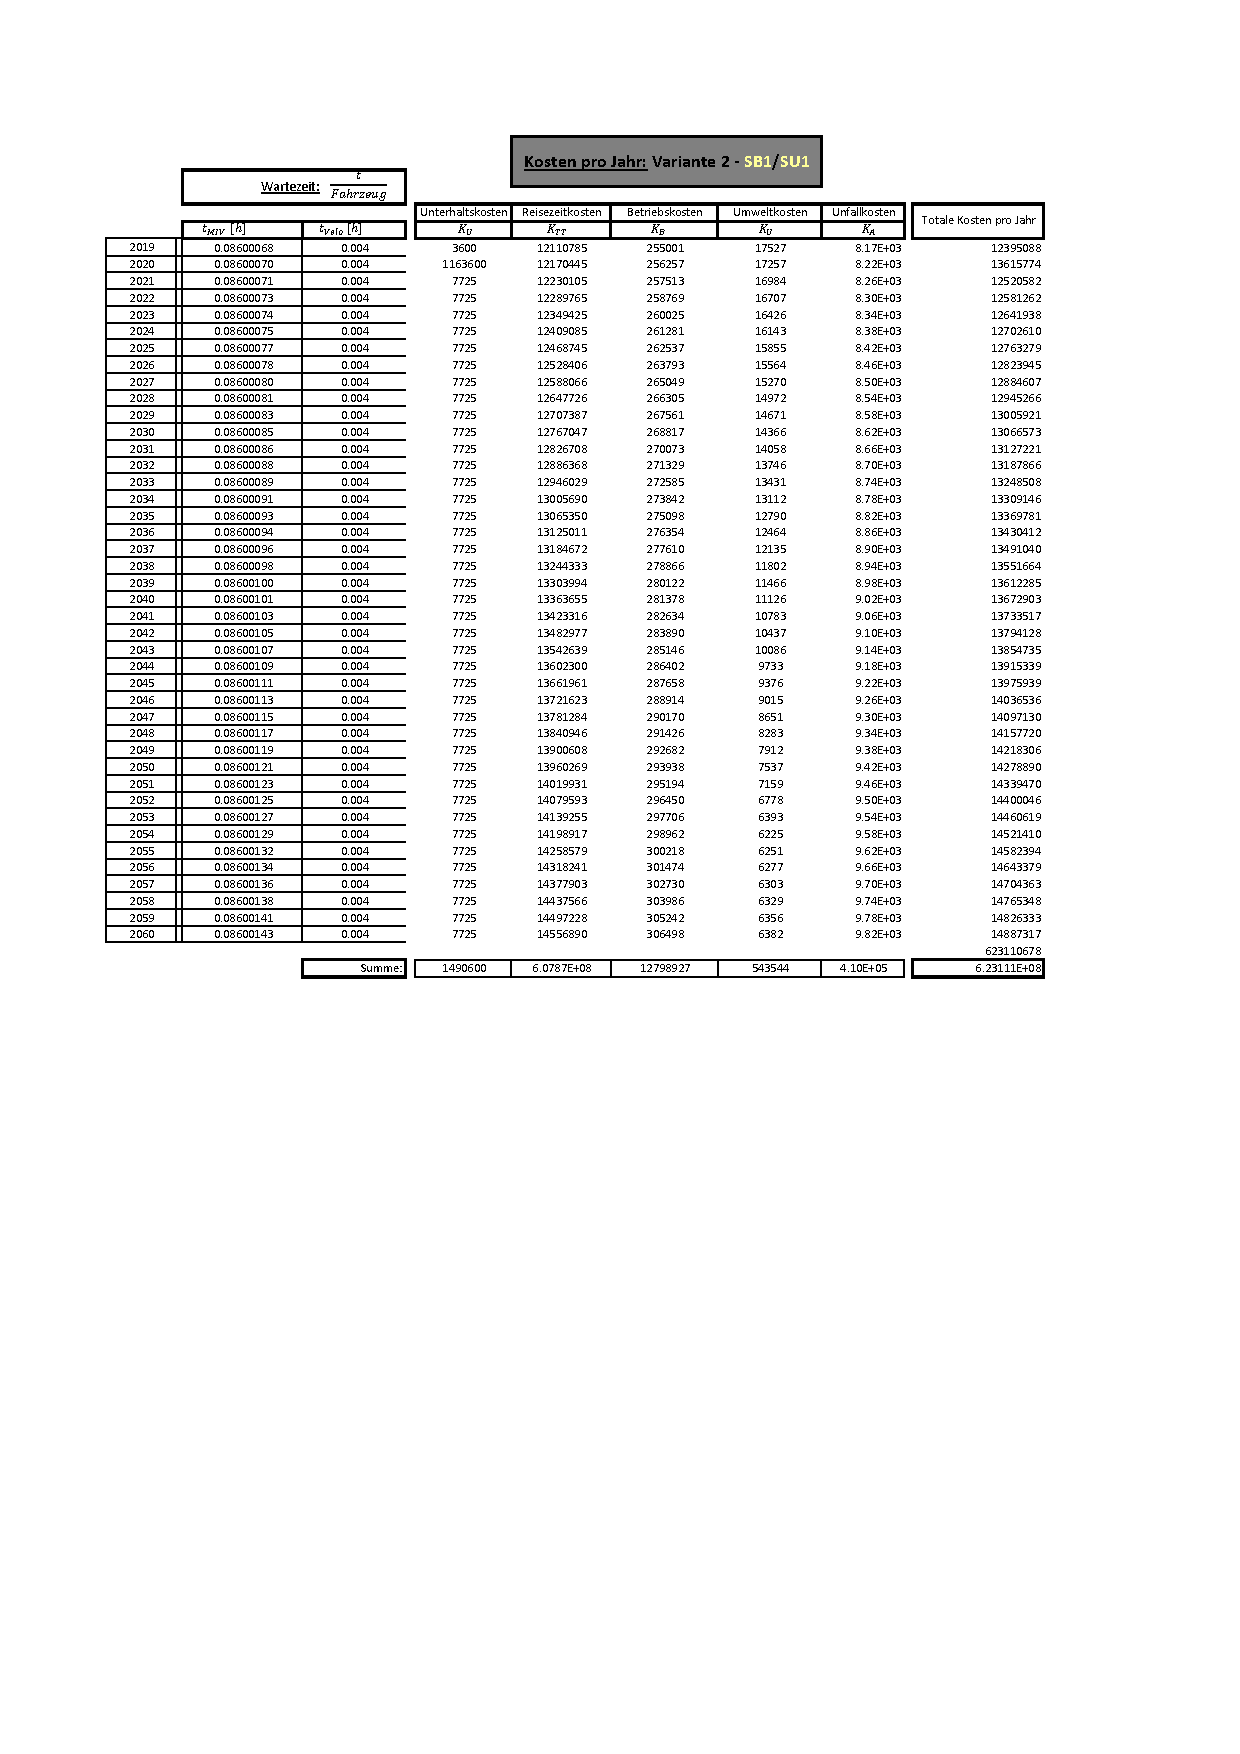
\includegraphics[width=\textwidth]{figures/Anhang/f-00-A-V2-B1-U1}
	\caption{Kostenberechung Variante 2 - SB1/SU1}
\end{figure}

\begin{figure}[h!]
	\centering
	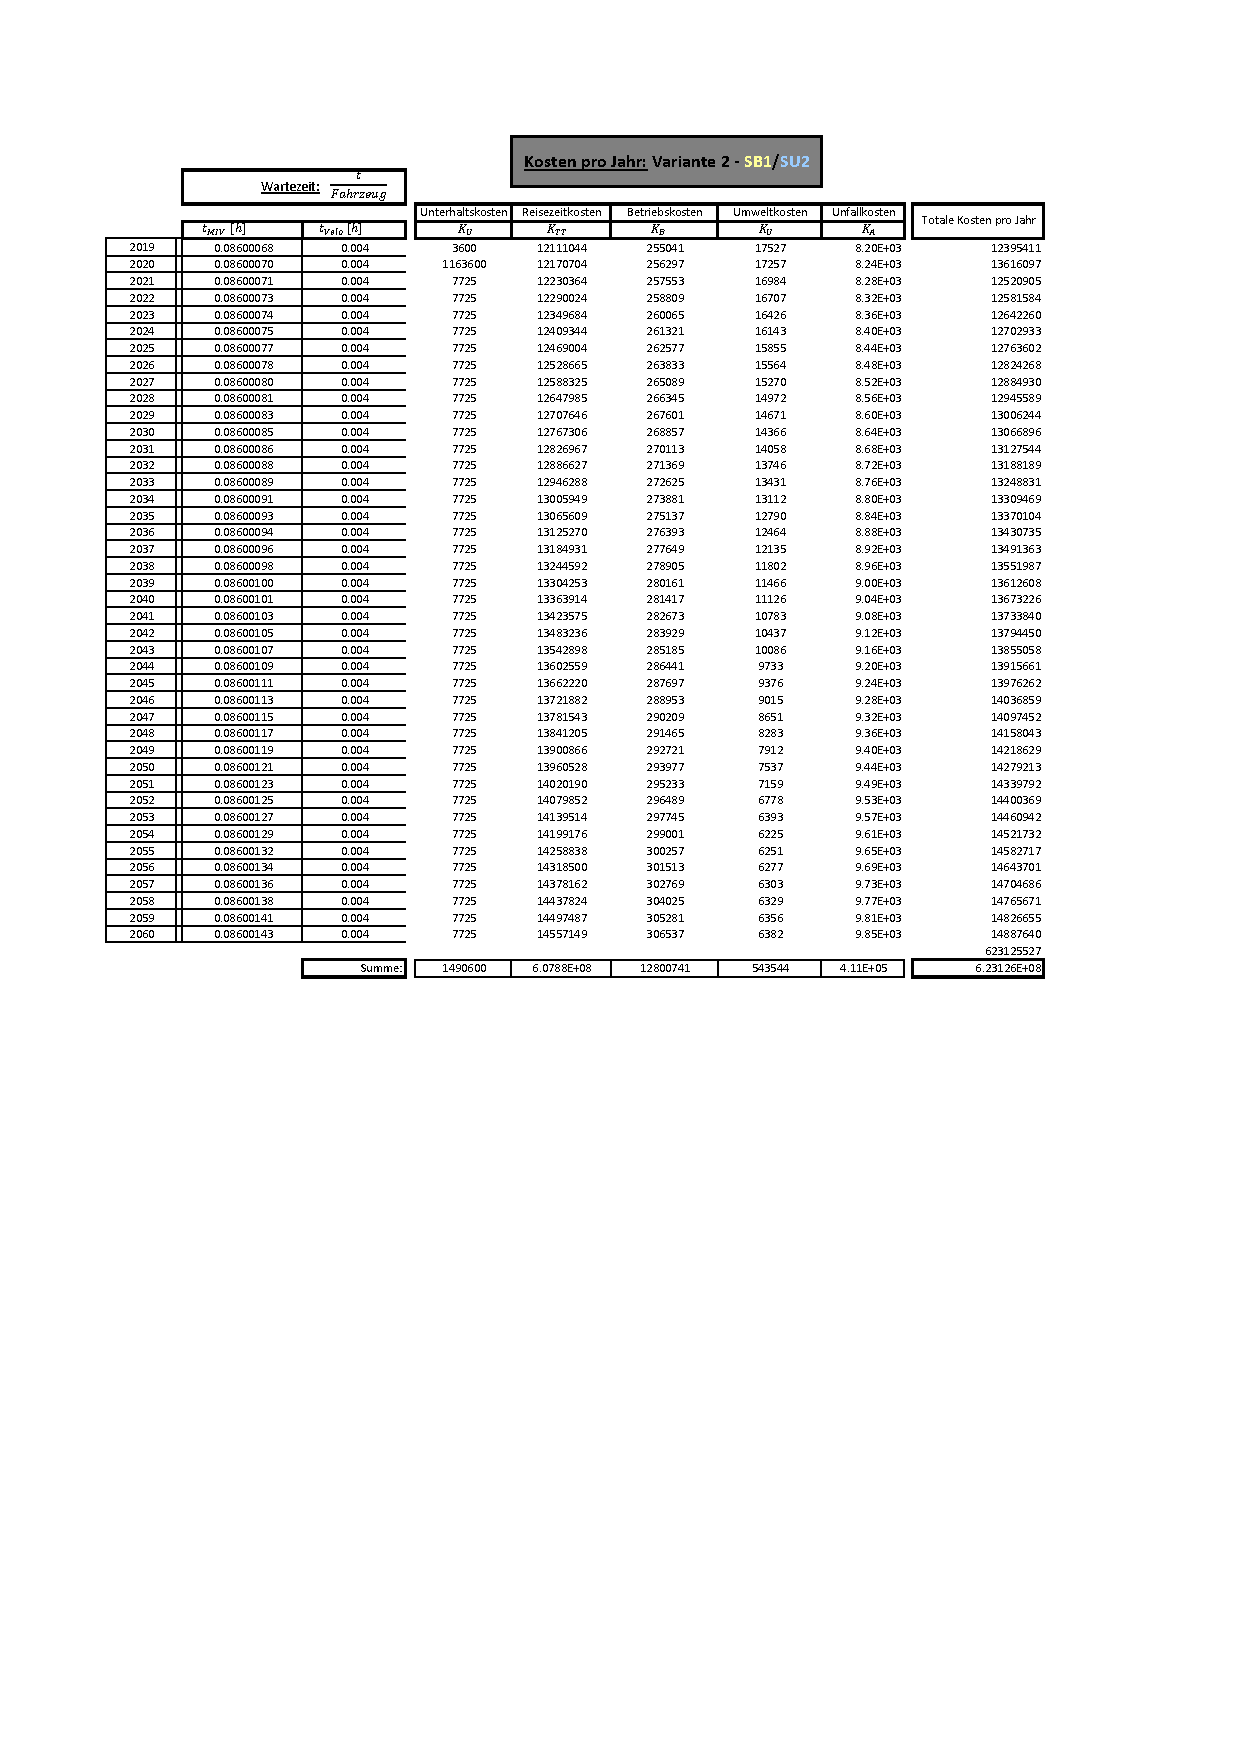
\includegraphics[width=\textwidth]{figures/Anhang/f-00-A-V2-B1-U2}
	\caption{Kostenberechung Variante 2 - SB1/SU2}
\end{figure}

\begin{figure}[h!]
	\centering
	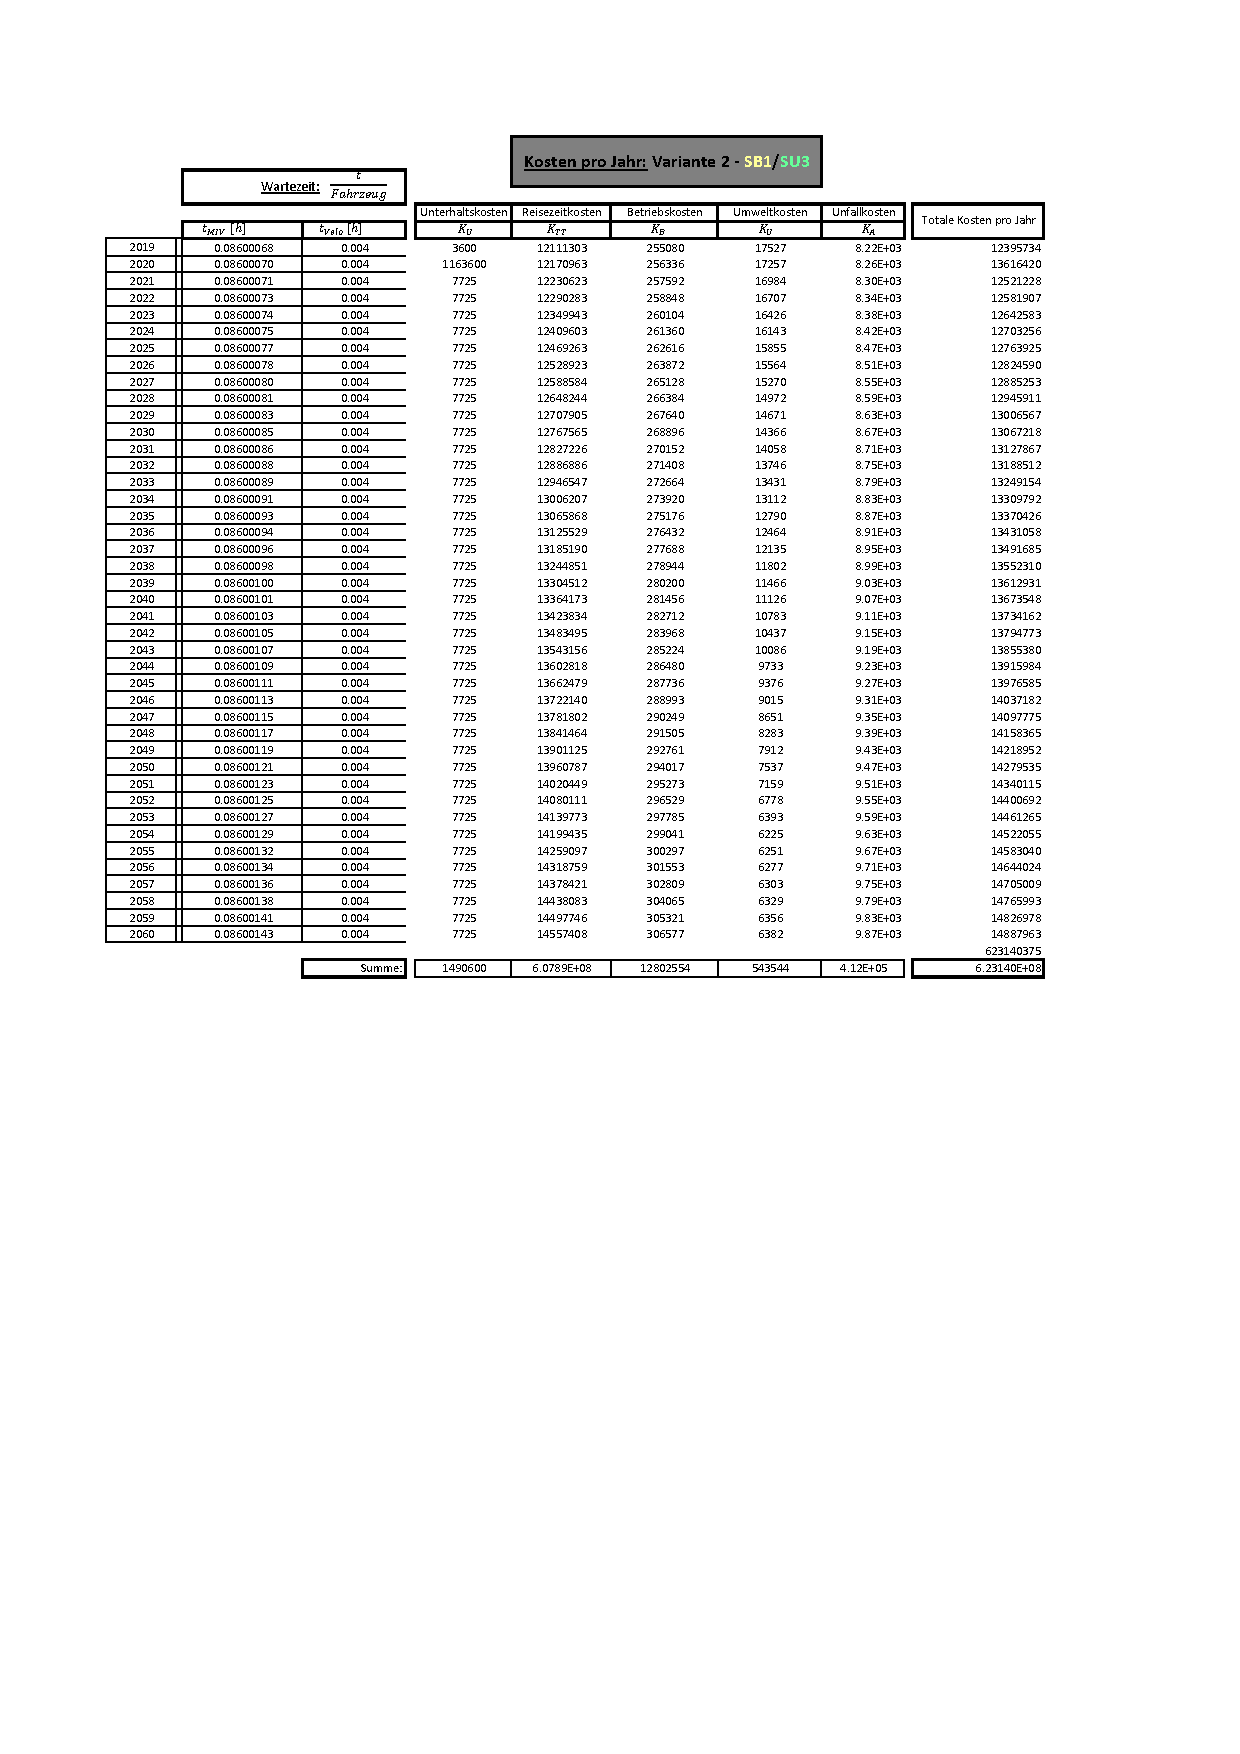
\includegraphics[width=\textwidth]{figures/Anhang/f-00-A-V2-B1-U3}
	\caption{Kostenberechung Variante 2 - SB1/SU3}
\end{figure}

\begin{figure}[h!]
	\centering
	\includegraphics[width=\textwidth]{figures/Anhang/f-00-A-V2-B2-U1}
	\caption{Kostenberechung Variante 2 - SB2/SU1}
\end{figure}

\begin{figure}[h!]
	\centering
	\includegraphics[width=\textwidth]{figures/Anhang/f-00-A-V2-B2-U2}
	\caption{Kostenberechung Variante 2 - SB2/SU2}
\end{figure}

\begin{figure}[h!]
	\centering
	\includegraphics[width=\textwidth]{figures/Anhang/f-00-A-V2-B2-U3}
	\caption{Kostenberechung Variante 2 - SB2/SU3}
\end{figure}

\begin{figure}[h!]
	\centering
	\includegraphics[width=\textwidth]{figures/Anhang/f-00-A-V2-B3-U1}
	\caption{Kostenberechung Variante 2 - SB3/SU1}
\end{figure}

\begin{figure}[h!]
	\centering
	\includegraphics[width=\textwidth]{figures/Anhang/f-00-A-V2-B3-U2}
	\caption{Kostenberechung Variante 2 - SB3/SU2}
\end{figure}

\begin{figure}[h!]
	\centering
	\includegraphics[width=\textwidth]{figures/Anhang/f-00-A-V2-B3-U3}
	\caption{Kostenberechung Variante 2 - SB3/SU3}
\end{figure}

\begin{figure}[h!]
	\centering
	\includegraphics[width=\textwidth]{figures/Anhang/f-00-A-V3-B1-U1}
	\caption{Kostenberechung Variante 3 - SB1/SU1}
\end{figure}

\begin{figure}[h!]
	\centering
	\includegraphics[width=\textwidth]{figures/Anhang/f-00-A-V3-B1-U2}
	\caption{Kostenberechung Variante 3 - SB1/SU2}
\end{figure}

\begin{figure}[h!]
	\centering
	\includegraphics[width=\textwidth]{figures/Anhang/f-00-A-V3-B1-U3}
	\caption{Kostenberechung Variante 3 - SB1/SU3}
\end{figure}

\begin{figure}[h!]
	\centering
	\includegraphics[width=\textwidth]{figures/Anhang/f-00-A-V3-B2-U1}
	\caption{Kostenberechung Variante 3 - SB2/SU1}
\end{figure}

\begin{figure}[h!]
	\centering
	\includegraphics[width=\textwidth]{figures/Anhang/f-00-A-V3-B2-U2}
	\caption{Kostenberechung Variante 3 - SB2/SU2}
\end{figure}

\begin{figure}[h!]
	\centering
	\includegraphics[width=\textwidth]{figures/Anhang/f-00-A-V3-B2-U3}
	\caption{Kostenberechung Variante 3 - SB2/SU3}
\end{figure}

\begin{figure}[h!]
	\centering
	\includegraphics[width=\textwidth]{figures/Anhang/f-00-A-V3-B3-U1}
	\caption{Kostenberechung Variante 3 - SB3/SU1}
\end{figure}

\begin{figure}[h!]
	\centering
	\includegraphics[width=\textwidth]{figures/Anhang/f-00-A-V3-B3-U2}
	\caption{Kostenberechung Variante 3 - SB3/SU2}
\end{figure}

\begin{figure}[h!]
	\centering
	\includegraphics[width=\textwidth]{figures/Anhang/f-00-A-V3-B3-U3}
	\caption{Kostenberechung Variante 3 - SB3/SU3}
\end{figure}
% ===========================================================================
% EOF
%

%%% Local Variables:
%%% mode: latex
%%% TeX-master: "../main"
%%% End:


% Index
% -----
\printindex

\end{document}

%=============================================================================
%%% Local Variables:
%%% mode: latex
%%% TeX-master: t
%%% End: